\documentclass[ngerman, openany, twoside]{texdata/Script}
\usepackage{amsmath}
\usepackage{pdfpages} % PDFs einbinden

% Aufgabentext ein-/ausschalten
\newboolean{aufgabentext}
\setboolean{aufgabentext}{true}
\newcommand{\aufgabentext}[1]{\ifthenelse{\boolean{aufgabentext}}{#1}{}}

% Wenn aufgabentext auch true ist, dann wird der Lösungstext etwas abgesetzt und kursiv geschrieben
\ifdefined\ishandout
  \newcommand{\loesung}[1]{\ifthenelse{\boolean{false}}{\ifthenelse{\boolean{aufgabentext}}{{\itshape{#1}}}{#1}}{}}
\else
  \newcommand{\loesung}[1]{\ifthenelse{\boolean{true}}{\ifthenelse{\boolean{aufgabentext}}{{\itshape{#1}}}{#1}}{}}
\fi

% Für die Strukturierung
\newcommand{\Thema}[1]{\chapter{#1}}
\newcommand{\Thementeil}[1]{\section{#1}}
\newcommand{\Aufgabe}[1]{\subsection{#1}}
\newcommand{\Unteraufgabe}[1]{\subsubsection{#1}}
\newcommand{\Lernziele}[1]{\subsection*{Lernziele}{#1}}
%\graphicspath{{./Bilder/}}

\newcommand{\mucho}[8]{
	\aufgabentext{
	\begin{enumerate}
	\item[#1] \emph{\textbf{#2}} #3
		\begin{enumerate}
		\itemsep1pt\parskip0pt\parsep0pt
		\item[A] #4
		\item[B] #5
		\item[C] #6
		\item[D] #7
		\end{enumerate}
		\loesung{Lösung: #8}
	\end{enumerate}
	}}

\begin{document}

%%%%%%%%%%%%%%%%%%%%%%%%%%%%%%%%%%%%%%%%%%%%%%%%%%%%%%%%%%%%%%%%%%%%%%%%
%% Head

% TODO Schicker machen & Leerseite danach

\titelseite[Christian Stoll\\ Sebastian Lange]{Skript AfuTUB-Kurs}%
  {Lizenzkurs der Amateurfunkgruppe der TU Berlin (AfuTUB/DK0TU)}%
  {WiSe 2017/18}%

\newpage
\thispagestyle{empty}

\hspace{.1cm}
\begin{minipage}[t]{13cm}

  \textbf{Impressum}\\

  \begin{tabular}{p{1cm} p{11cm}}
    Titel: &  Skript AfuTUB-Kurs (basierend auf dem Praxisskript der
    Projektwerkstatt "`Amateurfunk verbindet"', 2. Auflage März 2017)\\
    & \\
    Autoren: & Sebastian Lange, M.Sc. (Konzeption \& Praktische Anwendungen)\\
    & Christian Stoll, M.Ed. (Theorie- und Prüfungsfragen)\\
    %Abbildung:&\\
    & \\
    \multicolumn{2}{l}{Erschienen an der Technischen Universität Berlin:}\\
    &\\
    & Fachgebiet Hochfrequenztechnik (Sekr. HFT 4)\\
    & Institut für Hochfrequenz- und Halbleiter-Systemtechnologien\\
    & Fakultät IV -- Elektrotechnik und Informatik \\
    & Einsteinufer 25 \\
    & D-10587 Berlin \\
    & \\
    & Fachgebiet Raumfahrttechnik (Sekr. F 6)\\
    & Institut für Luft- und Raumfahrt\\
    & Fakultät V -- Verkehrs- und Maschinensysteme\\
    & Marchstraße 12-14\\
    & D-10587 Berlin\\
    &\\
    \multicolumn{2}{l}{1. Auflage Oktober 2018}\\
  \end{tabular}

  \vspace{3cm}

  Aktuelle Informationen der Amateurfunkgruppe der TU Berlin finden Sie unter:\\
  \url{https://dk0tu.de}

  \vspace{1cm}

  Die vorliegende Fassung des Skripts wurde sorgfältigst auf Fehler hin
  überprüft. Um das Skript dennoch laufend verbessern zu können, würden wir uns
  über Hinweise auf etwaig vorhandene Fehler sowie Verbesserungsvorschläge sehr
  freuen. Wenden Sie sich dazu bitte an die zuständigen Tutor*innen und
  wissenschaftlichen Mitarbeiter*innen.

\end{minipage}

% TODO acknowledgements Prof. Dr. Klaus Petermann / Brieß / Neuer Prof.

\newpage
%%Inhaltsverzeichnis
\tableofcontents
\newpage

%%%%%%%%%%%%%%%%%%%%%%%%%%%%%%%%%%%%%%%%%%%%%%%%%%%%%%%%%%%%%%%%%%%%%%%%
%% Inhalt

% TODO Aufteilung nach Technik und BV oder nach Lektionen?

\part{Technik Klasse E}

    % FIXME More Vorwort
    Die Technikkapitel des Moltrechts sind hier in zwei Teile aufgeteilt.
    Während die Vorlesung und das Buch auf das grundlegende Verständnis
    ausgerichtet sind, dienen die zusammengefassten \textbf{Theorie- und
    Prüfungsfragen} der konkreten Prüfungsvorbereitung und die
    \textbf{Praktischen Anwendungen} unterfüttern frisch erworbene Wissen.

\clearpage

\graphicspath{{e02-04_ET-Grundlagen/}}

\chapter{Spannung, Strom, Widerstand und Leistung (E02--E04)}

% FIXME Figure wieder oben richtig einbauen
% \begin{wrapfigure}[0]{r}[-1cm]{0.5cm}
%  \vspace{-7cm}
%   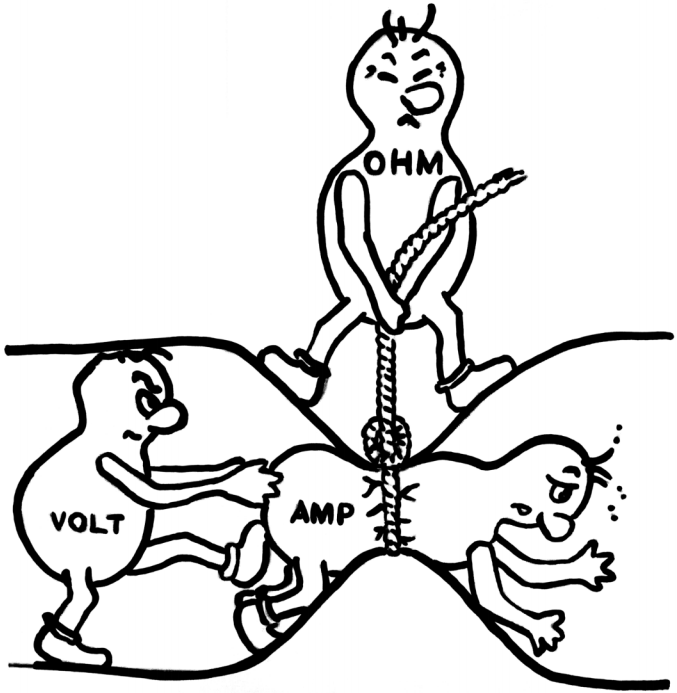
\includegraphics[scale=0.15]{e02-04_ET-Grundlagen/URI.png}
%  \vspace{-6cm}
% \end{wrapfigure}

%%%%%%%%%%%%%%%%%%%%%%%%%%%%%%%%%%%%%%%%%%%%%%%%%%%%%%%%%%%%%%%%%%%%%%%%
%% Theorie

\section{Theorie- und Prüfungsfragen}

%\loesung{
%\begin{figure}[H]
%\centering
%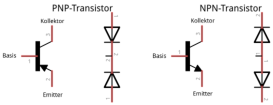
\includegraphics[scale=3]{Transistor/Bilder/PNP_NPN.pdf}
%\caption{1 und 2 - NPN- und PNP-Transistor}
%\end{figure}
%}

\mucho{1}{TB903}
{Welche Spannung lässt einen Strom von $2A$ durch einen Widerstand von
$50\Omega$ fließen?}%Frage
{$25V$}%A
{$200V$}%B
{$100V$}%C
{$52V$}%D
{C}%Lösung

\mucho{2}{TD302}
{Die Leerlaufspannung einer Gleichspannungsquelle beträgt $13,5V$. Wenn die
Spannungsquelle einen Strom von $1A$ abgibt, sinkt die Klemmenspannung auf
$12,4V$. Wie groß ist der Innenwiderstand der Spannungsquelle?}%Frage
{$1,1\Omega$}%A
{$1,2\Omega$}%B
{$12,4\Omega$}%C
{$13,5\Omega$}%D
{A}%Lösung

\mucho{3}{TB908}
{Ein mit einer künstlichen $50\Omega$-Antenne in Serie geschaltetes
HF-Amperemeter zeigt $2A$ an. Welche Leistung gibt der Sender ab?}%Frage
{$100W$}%A
{$200W$}%B
{$25\Omega$}%C
{$250\Omega$}%D
{B}%Lösung

\mucho{4}{TB104}
{Welche Gruppe von Materialien enthält nur Nichtleiter?}%Frage
{Pertinax, Polyvinylchlorid (PVC), Graphit}%A
{Epoxid, Polyethylen (PE), Polystyrol (PS)}%B
{Polyethylen (PE), Messing, Konstantan}%C
{Teflon, Pertinax, Bronze}%D
{B}%Lösung

\aufgabentext{
	\begin{enumerate}
	\item[5] \emph{\textbf{TC105-107}} Ordne den folgenden Schaltzeichen die Bezeichnungen LDR, PTC, NTC und VDR zu.\\
		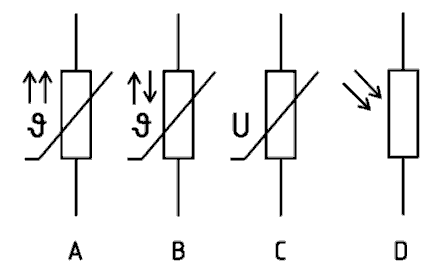
\includegraphics[scale=0.3]{Bild04.png}
		\loesung{Lösung: A PTC, B NTC, C VDR, D LDR}
		\end{enumerate}
	}

\mucho{6}{TC101}
{Die Farbringe gelb, violett und orange auf einem Widerstand mit 4 Farbringen bedeuten einen Widerstandswert von}%Frage
{$4,7k\Omega$}%A
{$47k\Omega$}%B
{$470k\Omega$}%C
{$4,7M\Omega$}%D
{gelb: 4; violett: 7; orange: $\cdot 10^3$; ergibt $47000\Omega$ oder $47k\Omega$: B}%Lösung

\mucho{7}{TC110}
{Welchen Wert hat ein SMD-Widerstand mit der Kennzeichnung 221?}%Frage
{$221\Omega$}%A
{$22k\Omega$}%B
{$22\Omega$}%C
{$220\Omega$}%D
{D}%Lösung

\mucho{8}{TC108}
{Ein Widerstand hat eine Toleranz von $10 \%$. Bei einem nominalen Widerstandswert von $5,6 k\Omega$ liegt der tatsächliche Wert zwischen}%Frage
{$4760$ und $6440 \Omega$}%A
{$5040$ und $6160 \Omega$}%B
{$4,7 k$ und $6,8 k\Omega$}%C
{$5,2 k$ und $6,3 k\Omega.$}%D
{B}%Lösung

\mucho{9}{TD108}
{Die Gesamtspannung U an folgendem Spannungsteiler beträgt $12,2V$. Die
Widerstände haben die Werte $R_1 = 10k\Omega$ und $R_2 = 2,2k\Omega$. Wie groß
ist die Teilspannung $U_2$?\\ 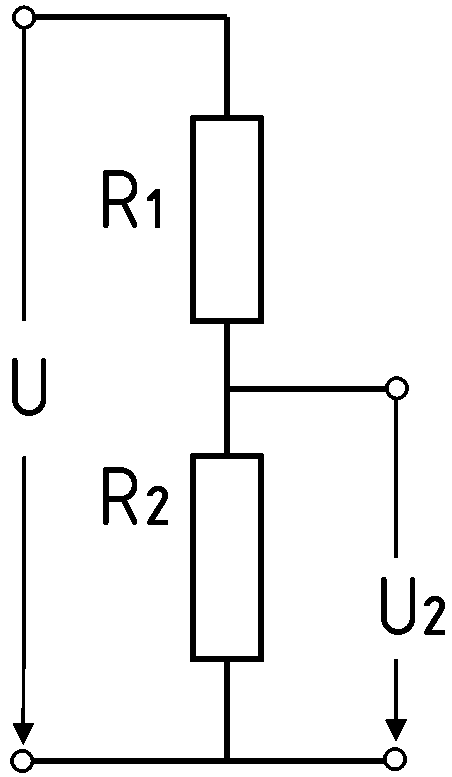
\includegraphics[scale=0.15]{Spannungsteiler.png}}%Frage
{$2,20V$}%A
{$2,64V$}%B
{$10,0V$}%C
{$1,22V$}%D
{A}%Lösung

\mucho{10}{TD103}
{Wie groß ist der Ersatzwiderstand der Gesamtschaltung? 
$R_1 = 500\Omega$, $R_2 = 500\Omega$ und $R_3 = 1k\Omega$\\ 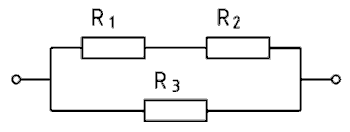
\includegraphics[scale=0.4]{Parallelschaltung.png}}%Frage
{$250\Omega$}%A
{$500\Omega$}%B
{$1k\Omega$}%C
{$2k\Omega$}%D
{B}%Lösung

%%%%%%%%%%%%%%%%%%%%%%%%%%%%%%%%%%%%%%%%%%%%%%%%%%%%%%%%%%%%%%%%%%%%%%%%
%% Praxis

\clearpage

\section{Grundlagen Breadboard/Messtechnik: U, I, R, P}

In diesem ersten Praxisteil Elektronik geht es darum euch mit dem Kursmaterial
vertraut zu machen und erste Schaltungen zu bauen und zu messen. Ablauf:

\begin{enumerate}
  \item Vorstellung des Kurskofferskonzepts und der Werkzeugtaschen
  \item Einführung Steckbrett
  \item Praxisaufgaben
\end{enumerate}

{
  \begin{wrapfigure}{r}{0.4\textwidth}
    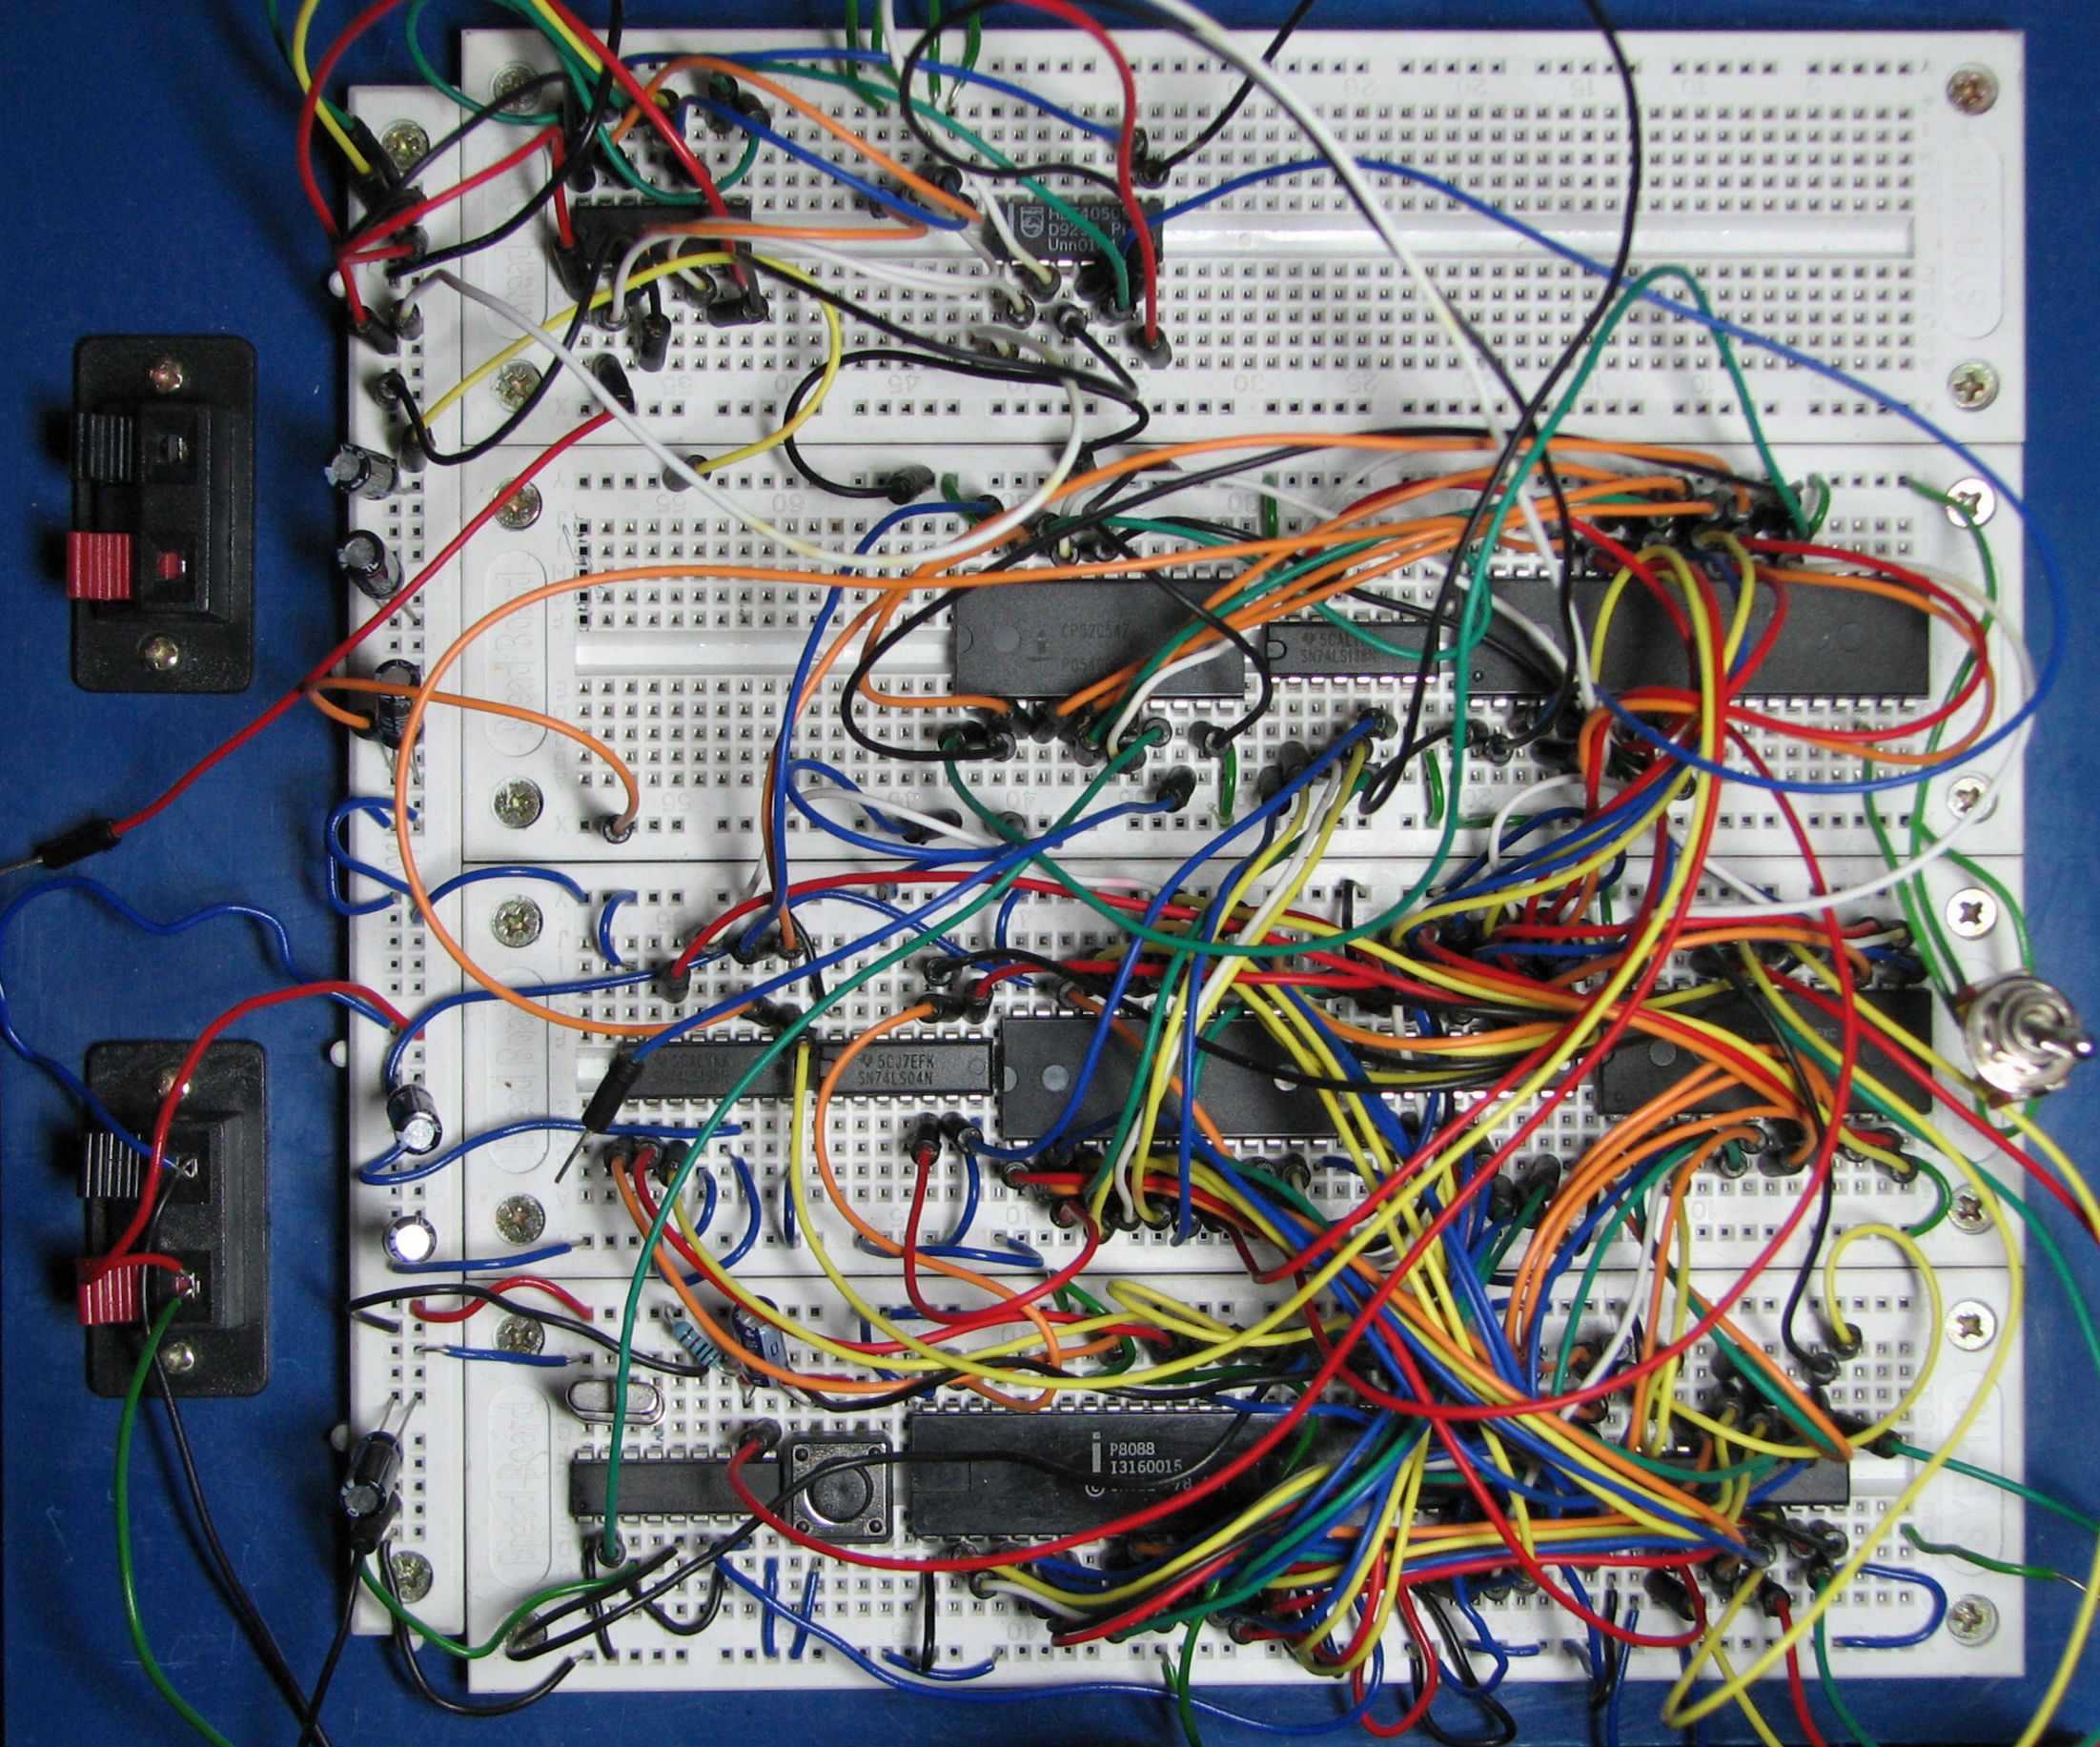
\includegraphics[width=0.38\textwidth]{Breadboard_complex.jpg}
  \end{wrapfigure}

  \paragraph{Vorbereitungsaufgabe}

  \emph{-- keine --}

  \loesung{Besondere Vorbereitungen: -- keine --}

  \paragraph{Material}

  \begin{itemize}
    \item[1x] Breadboard
    \item[1x] 9V-Blockbatterie oder 6--9V-Batteriefach
    \item[1x] LED
    \item[2x] Widerstand (unbekannt) \loesung{470 $\Omega$ \& 1k $\Omega$}
    \item Steckbrücken-/kabel
  \end{itemize}
}

\paragraph{Hinweise}

Achtet darauf die Pole des Batteriepacks nicht kurzzuschließen -- wird sehr heiß
und blubbert!

\paragraph{How to Breadboard}

Ein Breadboard bzw. Steckbrett erlaubt schnelle Versuche mit THT-Bauteilen. Die
Benutzung ist in Abbildung \ref{fig:breadboard} dargestellt.

\begin{figure}[htbp]
  \centering
  \subfigure[Leeres Breadboard]{
    \label{fig:breadboard_leer}
    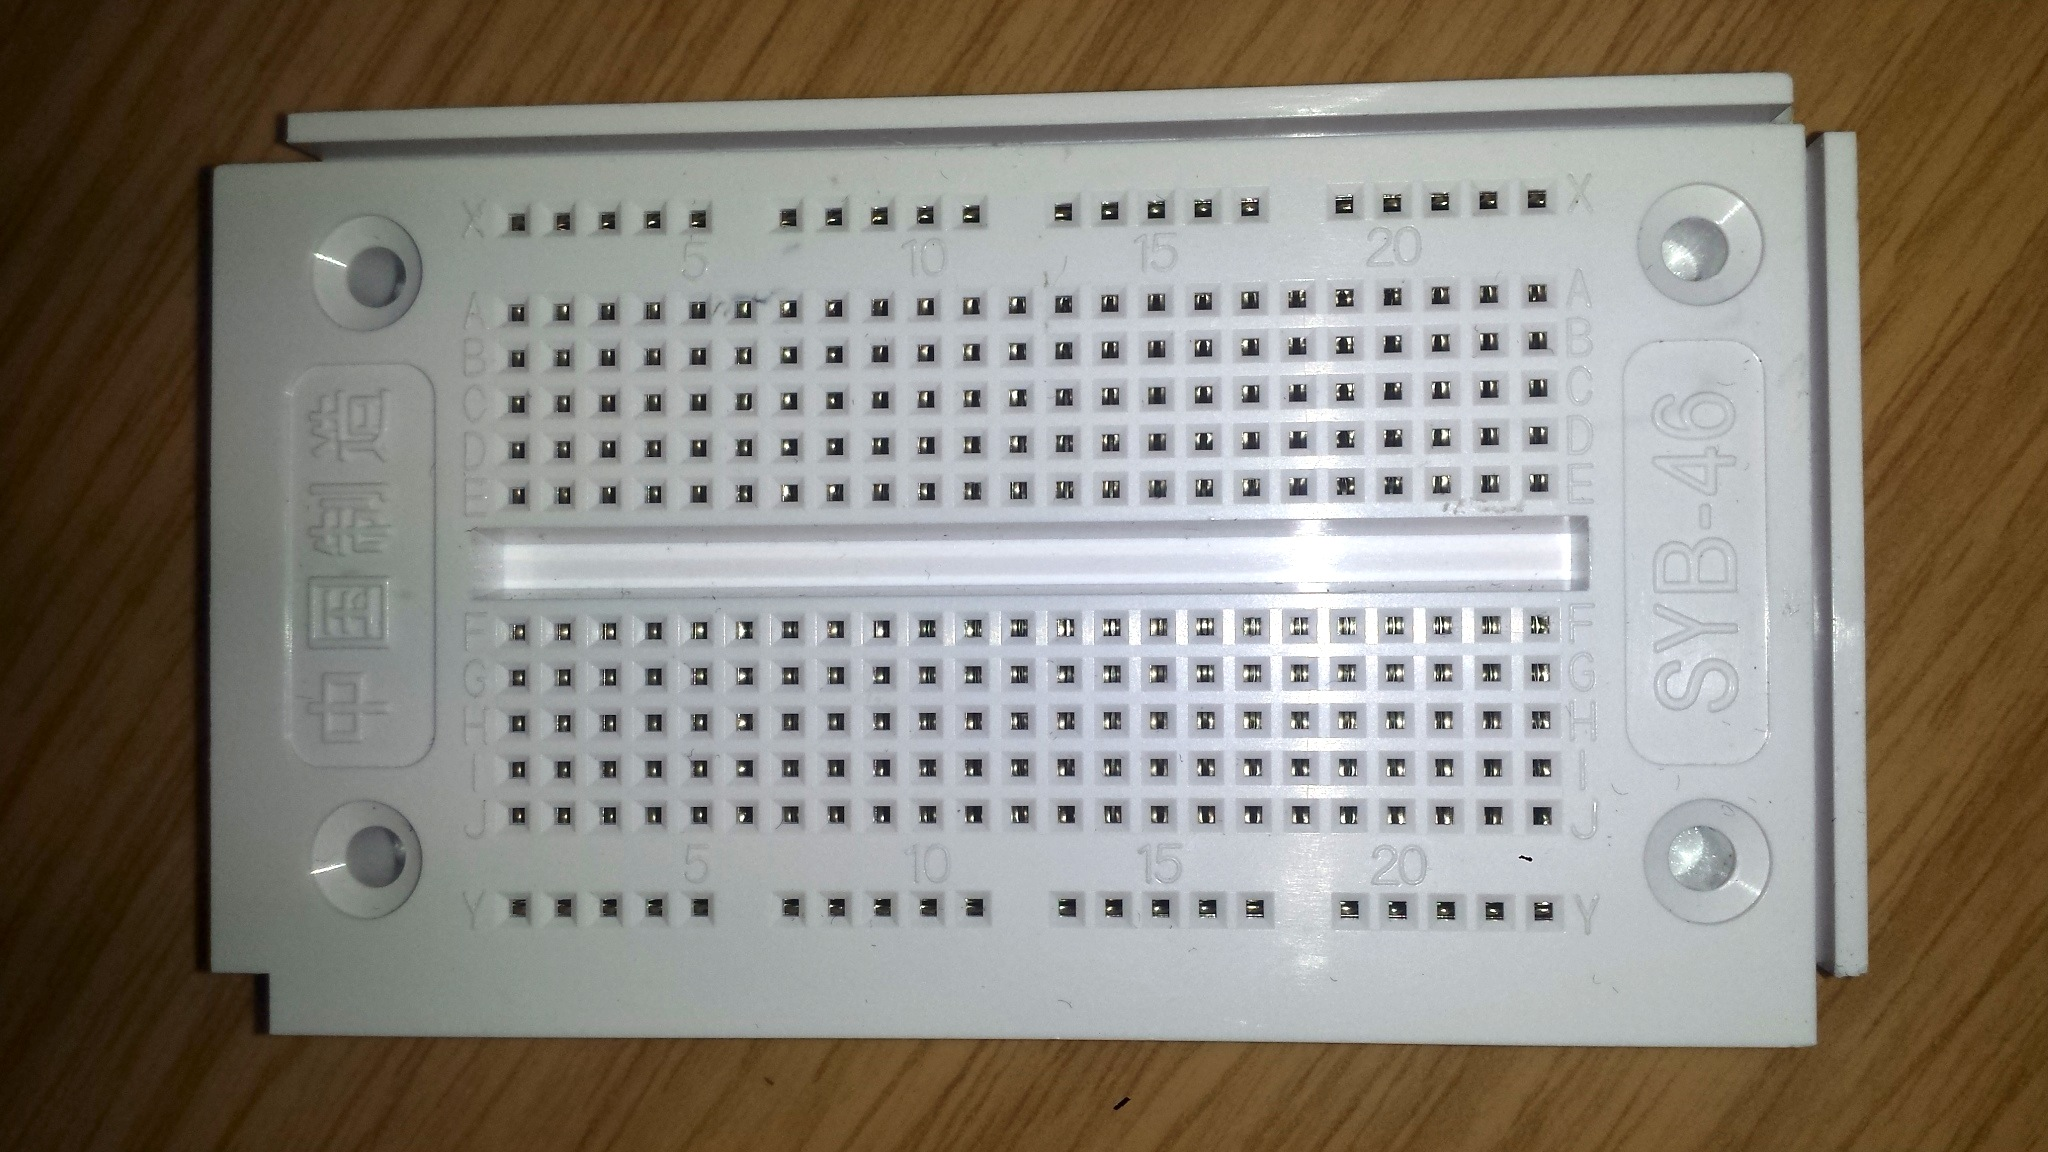
\includegraphics[width=0.3\textwidth]{Leeres_Board.jpg}
  }
  \subfigure[Bestückt mit Bauteilen]{
    \label{fig:breadboard_parts}
    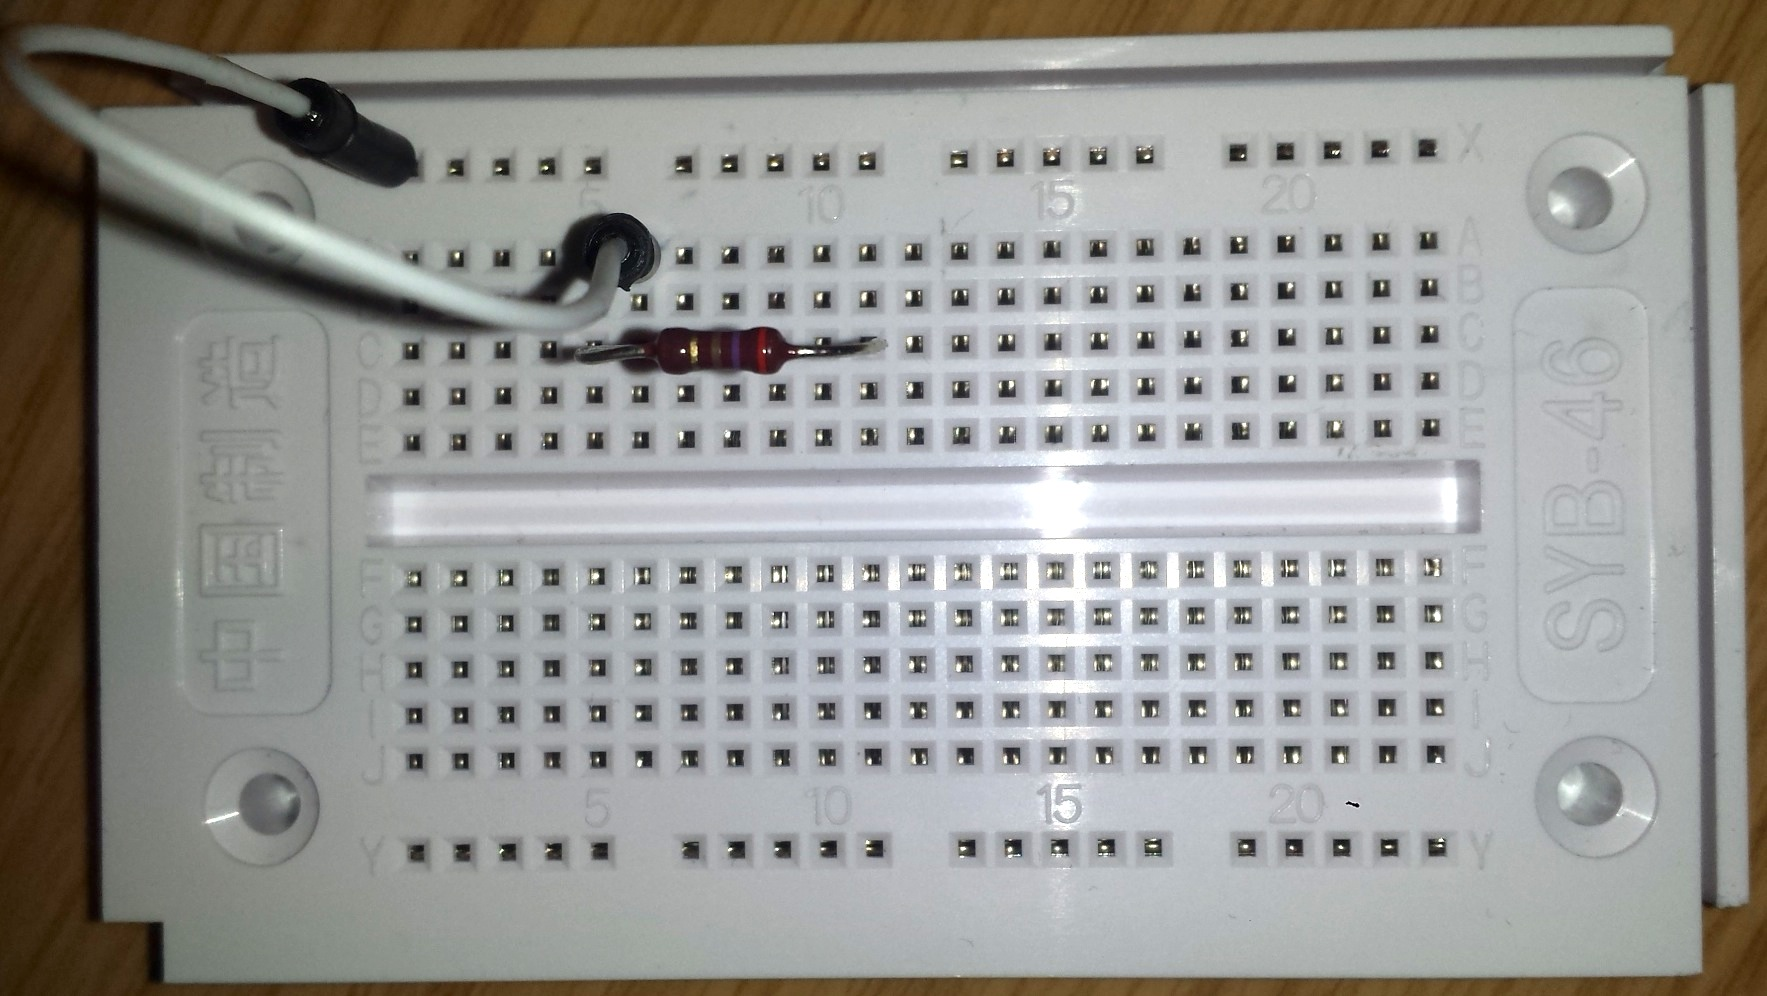
\includegraphics[width=0.3\textwidth]{Wiederstand_eingebaut.jpg}·
  }
  \subfigure[Verbindungen im Breadboard]{
    \label{fig:breadboard_lanes}
    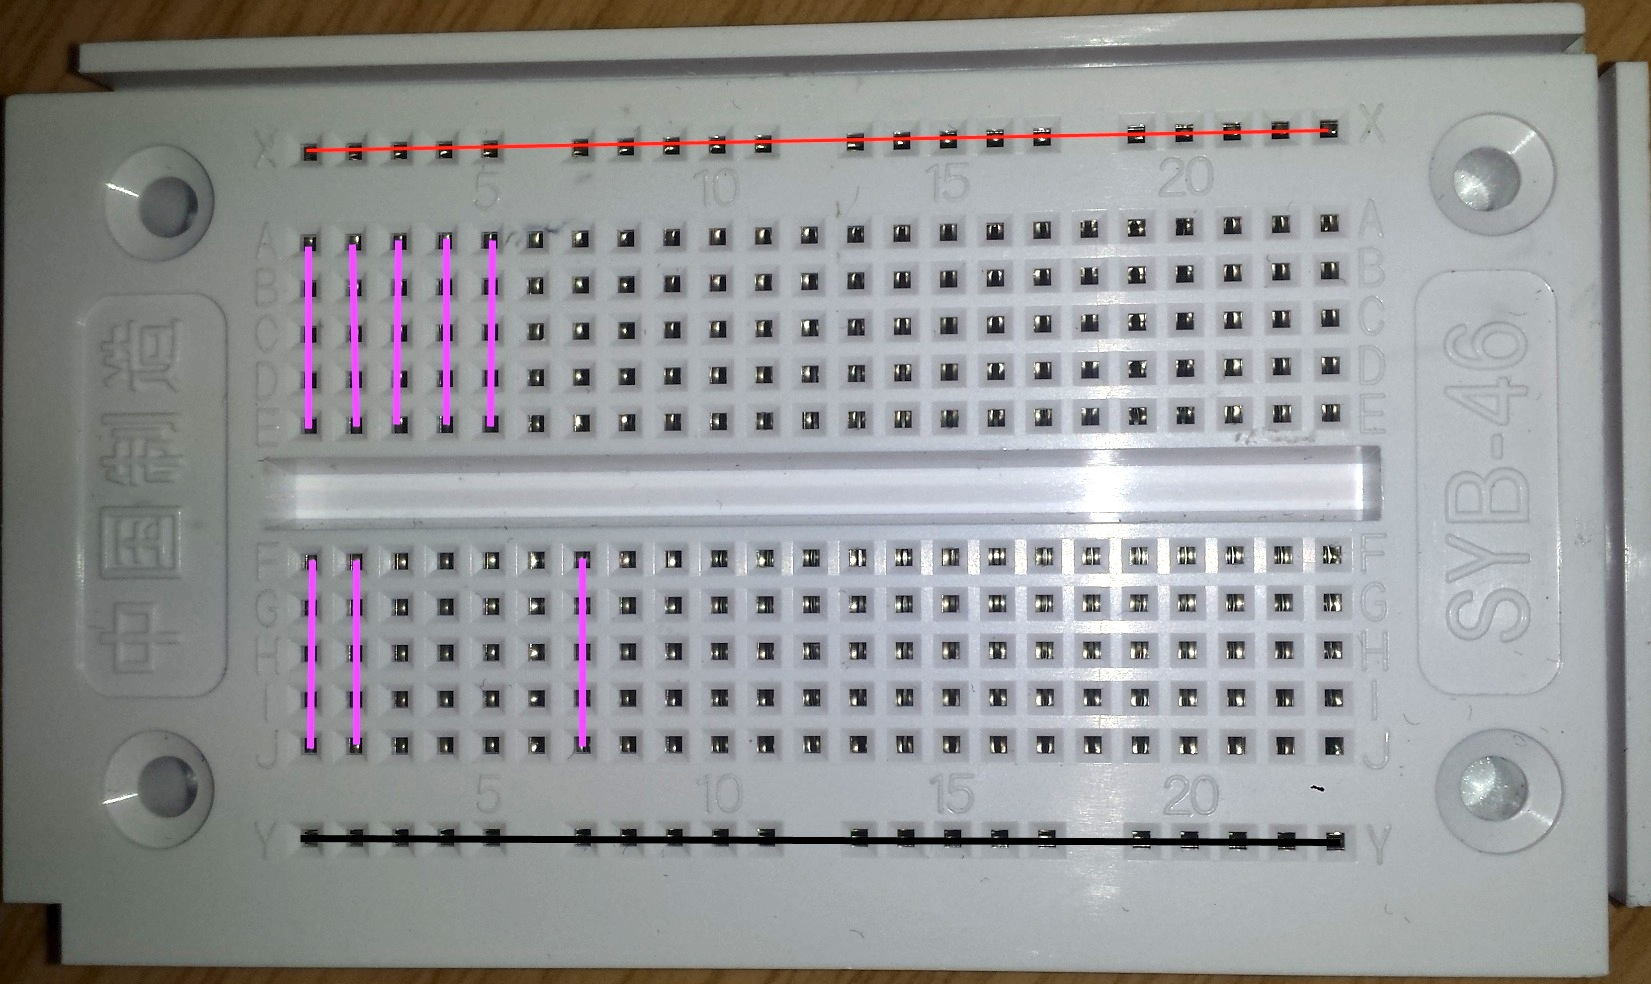
\includegraphics[width=0.5\textwidth]{Leeres_Board_verbindungen.jpg}
  }
  \caption{Mini-Breadboard SYB-46 \cite{afutub}} % FIXME citation
  \label{fig:breadboard}
\end{figure}

% TODO e99/Steckbrett_ersteUebung.png selber/gemeinsam stecken oder weglassen?

\clearpage

\paragraph{Aufgaben}

% DONE Schaltpläne einfügen? Nein, das muss so gehen.

\begin{enumerate}
  \item Wie ist ein übliches Batteriefach aufgebaut und wie verhalten sich dort
    Spannung und Strom? \\
    \loesung{Spannungen der Zellen addieren sich in Reihe, Strom überall
    gleich -- analog dazu: auch eine Batterie selbst ist meist eine gestapelte Zelle}
  \item Ihr habt zwei Widerstände zur Verfügung. Bestimmt die Bauteilwerte
    anhand der Ringe (vgl. Formelsammlungen im Anhang \ref{att:formela},
    \ref{att:formele} und \ref{att:formel+}) und messt sie nach.
    \begin{center}
    R1 = \dots \loesung{270} $\Omega$ \\
    R2 = \dots \loesung{1k} $\Omega$ \\
    Toleranz: 5\%
    \end{center}
  \item Baut einen Stromkreis mit einer LED und den beiden Vorwiderständen
    (einmal seriell, einmal parallel) auf dem Breadboard auf. Was ändert sich?
    Berechnet und messt jeweils den Gesamtvorwiderstand! \\
    \loesung{Parallel: 213 $\Omega$, Serie 1270 $\Omega$}
  \item Verwendet die parallele Gesamtschaltung für die weiteren Messungen
    \begin{enumerate}
      \item Messt die Einzelströme durch die Widerstände! Rechnet nach! \\
        \loesung{Messung: 270 $\Omega$: $\approx$ 20-30mA, 1k $\Omega$: $\approx$ 10 mA, $U_r$ = 6,65 V, $I_{ges} \approx $30 mA}\\
        \loesung{Rechnung: 270 $\Omega$: $\approx$ 24 mA, 1k $\Omega$: $\approx$ 6,6 mA, $I_{ges}$ = 31 mA}
      \item Messt die notwendigen Spannungen um die Leistungsaufnahme der
        Gesamtschaltung sowie der LED zu berechnen! Was fällt euch auf? \\
        \loesung{$I_{ges}$ = 30 mA, $U_{ges}$ = 9,11 V, $U_{LED}$ = 2,45 V, $P_{LED}$ = 73 mW, $P_{ges}$ = 273 mW, $\eta$ = 27\%}
    \end{enumerate}
  \item Zusatzaufgabe: Vorwiderstand LED\\ % FIXME siehe "Zusatzaufgabe" unten

\end{enumerate}

%%%%%%%%%%%%%%%%%%%%%%%%%%%%%%%%%%%%%%%%%%%%%%%%%%%%%%%%%%%%%%%%%%%%%%%%
%% Archiv: Aufgaben von DC4LW aus den alten Folien e04

%\subsection*{Übung 1}
%\begin{frame}
%  \begin{columns}
%    \column{0.4\textwidth}
%    \begin{center}
%      \begin{figure}
%        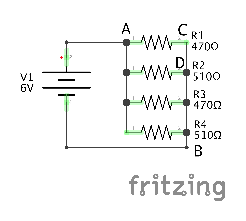
\includegraphics[width=1\textwidth]{e04/Uebung1_Schaltplan.pdf}
%      \end{figure}
%    \end{center}
%    \column{0.55\textwidth}
%    \begin{alertblock}{Aufgabe 1}
%      Baue die Schaltung auf dem Steckbrett auf.\\
%      Berechne den Ersatzwiderstand. Miss zur Überprüfung den Gesamtwiderstand.
%    \end{alertblock}
%    \begin{alertblock}{Aufgabe 2}
%      Berechne die Spannung über $R_1$, $R_2$, $R_3$ und $R_4$. Miss zur Überprüfung nach.\\
%      Miss und erkläre die Spannungen über $A$---$B$, $A$---$C$ und $A$---$D$.
%    \end{alertblock}
%  \end{columns}
%  \begin{alertblock}{Aufgabe 3}
%    Berechne die Ströme durch $R_1$, $R_2$, $R_3$, $R_4$ und den Gesamtstrom. Miss zur %Überprüfung nach.
%  \end{alertblock}
%\end{frame}

%\subsection*{Übung 2}
%\begin{frame}
%  \begin{columns}
%    \column{0.4\textwidth}
%    \begin{center}
%      \begin{figure}
%        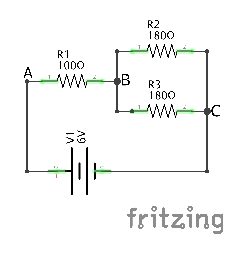
\includegraphics[width=1\textwidth]{e04/Uebung2_Schaltplan.pdf}
%      \end{figure}
%    \end{center}
%    \column{0.55\textwidth}
%    \begin{alertblock}{Aufgabe 1}
%      Baue die Schaltung auf dem Steckbrett auf.
%      Berechne den Ersatzwiderstand. Miss zur Überprüfung den Gesamtwiderstand.
%    \end{alertblock}
%    \begin{alertblock}{Aufgabe 2}
%      Berechne die Spannung über $R_1$, $R_2$ und $R_3$. Miss zur Überprüfung nach.\\
%      Miss und erkläre die Spannungen über $A$---$B$, $A$---$C$ und $B$---$C$.
%    \end{alertblock}
%  \end{columns}
%  \begin{alertblock}{Aufgabe 3}
%    Berechne die Ströme durch $R_1$, $R_2$, $R_3$ und den Gesamtstrom. Miss zur Überprüfung %nach.
%  \end{alertblock}
%\end{frame}

%\subsection*{Übung 3}
%\begin{frame}
%  \begin{alertblock}{Zusatzaufgabe}
%    Die rote Leuchtdiode benötigt einen Strom von $20mA$. Für die Aufgabe sei erstmal angenommen, dass keine Spannung über die Leuchtdiode abfällt. Dimensioniere einen Spannungsteiler so, dass mit der gegebenen Batterie von 6V an der Leuchtdiode eine Spannung von 3V bis 5V anliegt. Gegeben sind die Widerstände in der Größe $4\times100\Omega$, $2\times180\Omega$, $4\times470\Omega$ und $2\times510\Omega$. Berechne zuerst den Spannungsteiler und zeichne einen Schaltplan.
%  \end{alertblock}
%%  \begin{alertblock}{Aufgabe 2}
%%    Baue die Schaltung auf. Die abgeflachte Seite der Leuchtdiode zeigt zu Minus. Miss den %Strom durch die Leuchtdiode. Miss die Spannung über die Widerstände. Wie lautet die %Gesamtsumme der Spannungen über die Widerstände? Erkläre.
%%  \end{alertblock}
%%  \begin{alertblock}{Aufgabe 3}
%%    Die Leuchtdiode soll dunkler leuchten. Muss dazu mehr oder weniger Strom fließen? Wie %sind die Widerstände zu dimensionieren?
%%  \end{alertblock}
%\end{frame}

\graphicspath{{e05_Kondensator/}}

\clearpage
\begin{minipage}{0.8\textwidth}
  \chapter{Der Kondensator (E05)}
\end{minipage}
\begin{minipage}{0.2\textwidth}
  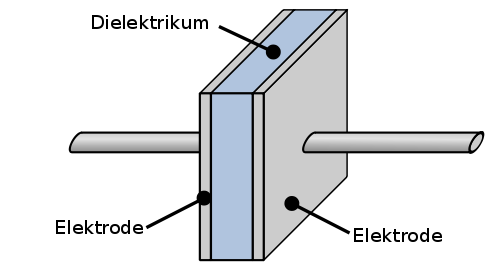
\includegraphics[width=0.9\textwidth]{Kondensator.png}
  \footnotemark
\end{minipage}
\footnotetext{Quelle unbekannt} % FIXME

%%%%%%%%%%%%%%%%%%%%%%%%%%%%%%%%%%%%%%%%%%%%%%%%%%%%%%%%%%%%%%%%%%%%%%%%
%% Theorie

\section{Theorie- und Prüfungsfragen}

\mucho{1}{TC206}
{
Drei Kondensatoren mit den Kapazitäten $C_1 = 0,1\mu F$, $C_2 = 150nF$ und $C_3 = 50000pF$ werden parallel geschaltet. Wie groß ist die Gesamtkapazität?
}%Frage
{$0,027\mu F$}%A
{$0,255\mu F$}%B
{$0,3\mu F$}%C
{$2,73nF$}%D
{C; $C_g = 100nF + 150nF + 50nF = 300nF = 0,3\mu F$}%Lösung


\mucho{2}{TD105}
{
Berechnen Sie die Gesamtkapazität der gemischten Schaltung.\\
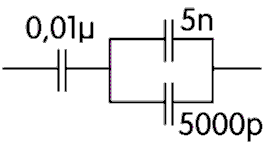
\includegraphics[scale=0.35]{TD105.png}
}%Frage
{$0,015nF$}%A
{$5nF$}%B
{$7,5nF$}%C
{$10nF$}%D
{B; $C_g = \dfrac{C_1 \cdot C_{2+3}}{C_1 + C_{2+3}} = \dfrac{10nF \cdot (5nF + 5nF)}{10nF + (5nF + 5nF)} = 5$}%Lösung

\mucho{3}{TD106}
{
Berechnen Sie die Gesamtkapazität der gemischten Schaltung. Gegeben: $C1 = 0,02\mu F$; $C2 = 10nF$; $C3 = 10000pF $ \\
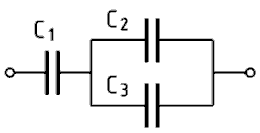
\includegraphics[scale=0.35]{TD106.png}
}%Frage
{$2,5nF$}%A
{$5nF$}%B
{$10nF$}%C
{$40nF$}%D
{C; $C_g = \dfrac{C_1 \cdot C_{2+3}}{C_1 + C_{2+3}} = \dfrac{20nF \cdot (10nF + 10nF)}{20nF + (10nF + 10nF)} = 10nF$}%Lösung

\mucho{4}{TD107}
{
Berechnen Sie die Gesamtkapazität der gemischten Schaltung. Gegeben: $C1 = 0,01 \mu F$; $C2 = 10 nF$; $C3 = 5000 pF$\\
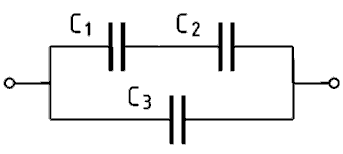
\includegraphics[scale=0.3]{TD107.png}
}%Frage
{$2,5 nF$}%A
{$5 nF$}%B
{$10 nF$}%C
{$0,015 nF$}%D
{C; $C_g = \dfrac{C_1 \cdot C_2}{C_1 + C_2} + C_3 = \dfrac{10nF \cdot 10nF}{10nF + 10nF} + 5nF = 10nF$}%Lösung

\mucho{5}{TC208}
{Mit zunehmender Frequenz}%Frage
{steigt der Wechselstromwiderstand des Kondensators.}%A
{sinkt der Wechselstromwiderstand des Kondensators.}%B
{steigt der Wechselstromwiderstand des Kondensators bis zu einem Maximum und sinkt dann wieder.}%C
{sinkt der Wechselstromwiderstand des Kondensators bis zu einem Minimum und steigt dann wieder.}%D
{B; $X_C = \dfrac{1}{2\pi \cdot f \cdot C}$}%Lösung


\mucho{6}{TC201}
{Welche Aussage zur Kapazität eines Plattenkondensators ist richtig?}%Frage
{Je größer die angelegte Spannung ist, desto kleiner ist die Kapazität.}%A
{Je größer die Dielektrizitätszahl ist, desto kleiner ist die Kapazität.}%B
{Je größer die Plattenoberfläche ist, desto kleiner ist die Kapazität.}%C
{Je größer der Plattenabstand ist, desto kleiner ist die Kapazität.}%D
{D}%Lösung

\mucho{7}{TC202}
{Ein Bauelement, bei dem sich Platten auf einer isolierten Achse befinden, die zwischen fest stehende Platten hineingedreht werden können, nennt man}%Frage
{Drehkondensator.}%A
{Tauchkondensator.}%B
{Keramischer Kondensator.}%C
{Rotorkondensator.}%D
{A}%Lösung

\mucho{8}{TC207}
{Bei welchem der folgenden Bauformen von
Kondensatoren muss beim Einbau auf die
Polarität geachtet werden?}%Frage
{Elektrolytkondensator}%A
{Keramischer Kondensator}%B
{Styroflexkondensator}%C
{Plattenkondensator}%D
{A}%Lösung

\mucho{9}{TC203}
{Welche Kapazität hat der abgebildete Kondensator?\\
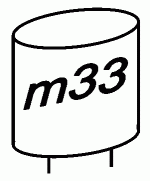
\includegraphics[width=1.1cm]{TC203.png}
}%Frage
{$3,3\mu F$}%A
{$33\mu F$}%B
{$33000\mu F$}%C
{$330\mu F$}%D
{D}%Lösung

\mucho{10}{TC205}
{Welche Kapazität hat der abgebildete Kondensator?\\
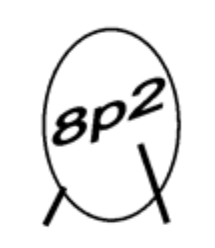
\includegraphics[width=1.1cm]{TC205.png}
}%Frage
{$820pF$}%A
{$8,2pF$}%B
{$82pF$}%C
{$0,82pF$}%D
{B}%Lösung

%%%%%%%%%%%%%%%%%%%%%%%%%%%%%%%%%%%%%%%%%%%%%%%%%%%%%%%%%%%%%%%%%%%%%%%%
%% Praxis

\clearpage

\section{Kapazität}

Der Kondenstator steht als Bauteil stelltvertretend für das Phänomen der
elektischen Kapazität. Im Folgenden soll dieser weiter praktisch untersucht
werden.

\paragraph{Vorbereitungsaufgabe}

\emph{-- fakultativ --} Baut aus irgendetwas einen Kondensator und bringt ihn mit.
Vielleicht findet ihr auch noch einen interessanten Kondensator in eurer
Bastelkiste?

\loesung{Besondere Vorbereitungen: Einen großen DrehKo mitbringen zur
Anschauung.}

\paragraph{Material}

% TODO ergänzen
\begin{itemize}
  \item[1x] ModulBus VCap4 (Datenblatt Anlage \ref{att:vcap})
  \item[1x] LC-Meter (Manual Anlage \ref{att:ae20204})
  \item \dots
\end{itemize}

\paragraph{Hinweise}

%FIXME Bedienungsanleitung in die Anlage
Sorgfältig mit den Messgeräten umgehen. Vorher Bedienungsanleitung lesen,
warmlaufen lassen und kalibrieren!

\paragraph{Aufgaben}

% TODO Aufgaben verbessern!
\begin{enumerate}
    \item Betrachtung des Drehkondensators ModulBus VCap4.
    \begin{enumerate}
      \item Was bedeutet VCap?\\
        \loesung{Variable Capacity}
      \item Wie funktioniert der vorliegende DrehKo?\\
        \loesung{Kapazitätsänderung durch Flächenänderung}
      \item Was machen die Trimmer?\\
        \loesung{}
      \item Welche maximale Kapazität bekommt man aus dem Bauteil?\\
        $C_{max} = \dots$ \loesung{}
      \item Welche minimale Kapazität (einstellbar) bekommt man aus dem
        Bauteil?\\
        $C_{min} = \dots$ \loesung{}
    \end{enumerate}
  \item Was gibt es noch so an Kondensatoren? $\rightarrow$ C bauen, berechnen, messen
  %FIXME Funktioniert die Aufgabe? Wechselstromwiderstand relevant für Klasse E?
  \item Wechselstromwiderstand: NF-AC mit Smartphone erzeugen und Durchgänge
    Kondensator + Lämpchen/Lautsprecher testen
\end{enumerate}


\part{unbearbeitet}


%https://de.wikipedia.org/wiki/Datei:Electronic_component_inductors.jpg

\begin{wrapfigure}[0]{r}[-1cm]{3cm}
 \vspace{-5cm}
 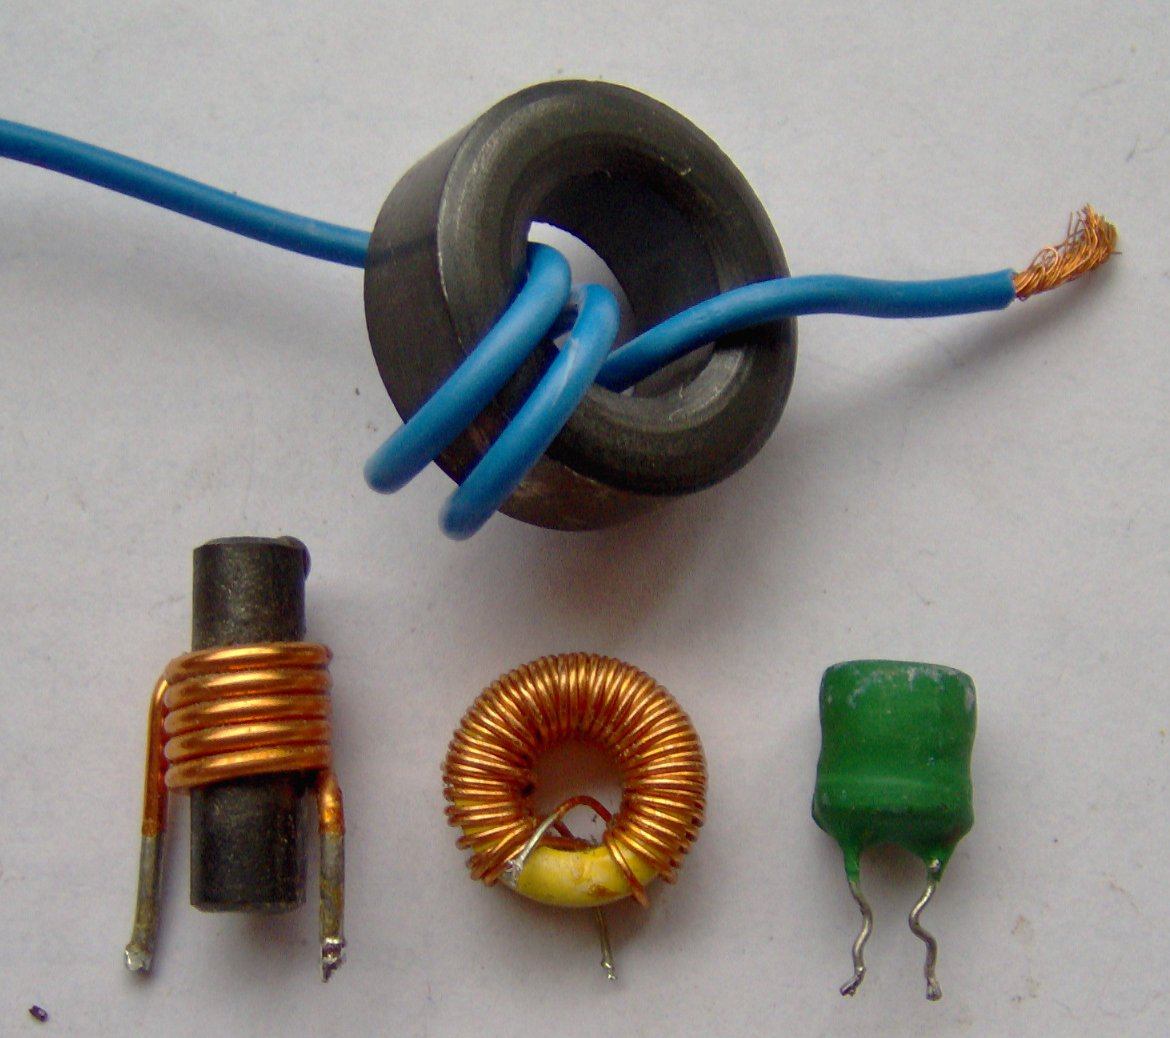
\includegraphics[scale=0.1]{Spule/Bilder/Electronic_component_inductors.jpg}
 \vspace{-5cm}
\end{wrapfigure}

\section*{Theorie- und Prüfungsfragen} 
~~~
\begin{enumerate}
\itemsep1pt\parskip0pt\parsep0pt
\item[1] Wie lässt sich die Induktivität einer Spule berechnen?
\item[2] Wie lautet die magnetische Feldkonstante $\mu_0$?
\item[3] Wie lautet die relative Permeabilität $\mu_r$ für Luft?
\item[4] Berechne die Induktivität der Zylinderspule mit folgender Bemaßung: 25 Windungen, 	Durchmesser von 8mm, Länge 1cm, relative Permeabilität von Luft
\end{enumerate}

\loesung{
	\begin{align}
	i) ~& L ~&=&~ & \dfrac{\mu_0 \cdot \mu_r \cdot A \cdot N^2}{l}\\
	ii) ~& \mu_0 ~&=&~ & 1,2566\cdot 10^{-6} \frac{H}{m}\\
	iii) ~& \mu_{r, Luft} ~& = &~ & 1 + 4 \cdot 10^{-7}\\
	iv) ~& L ~&=&~& 3,9\mu H
	\end{align}
	}

%\begin{block}
\aufgabentext{
	\begin{enumerate}
	\item[5] \emph{\textbf{TB402}}  Wie nennt man das Feld im Innern einer langen Zylinderspule beim Fließen eines Gleichstroms?
		\begin{enumerate}
		\itemsep1pt\parskip0pt\parsep0pt
		\item[A] Homogenes elektrisches Feld
		\item[B] Zentriertes magnetisches Feld
		\item[C] Konzentrisches Magnetfeld
		\item[D] Homogenes magnetisches Feld 
		\loesung{Lösung: D}
		\end{enumerate}
	\end{enumerate}
}

%\end{block}

%\begin{block}
\aufgabentext{
	\begin{enumerate}
	\item[6] \emph{\textbf{TC302}} Wie ändert sich die Induktivität einer Spule von $12 \mu H$, wenn die Wicklung auf dem Wickelkörper bei gleicher Windungszahl auf den doppelten Wert auseinander gezogen wird?
		\begin{enumerate}
		\itemsep1pt\parskip0pt\parsep0pt
			\item[A] Die Induktivität sinkt auf $3 \mu H$.
			\item[B] Die Induktivität sinkt auf $6 \mu H$. 
			\item[C] Die Induktivität steigt auf $24 \mu H$.
			\item[D] Die Induktivität steigt auf $48 \mu H$.
			\loesung{Lösung: B}
		\end{enumerate}	
	\end{enumerate}	
%\end{block}
}
%\begin{block}
\aufgabentext{
	\begin{enumerate}
		\item[7] \emph{\textbf{TC303}} Wie kann man die Induktivität einer Spule vergrößern?
		\begin{enumerate}
		\itemsep1pt\parskip0pt\parsep0pt
			\item[A] Durch Auseinanderziehen der Spule (Vergrößerung der Spulenlänge).
			\item[B] Durch Einführen eines Kupferkerns in die Spule.
			\item[C] Durch Stauchen der Spule (Verkürzen der Spulenlänge). 
			\item[D] Durch Einbau der Spule in einen Abschirmbecher.
			\loesung{Lösung: C}
		\end{enumerate}
	\end{enumerate}
%\end{block}
}



\mucho{8}{TC305}
{Schaltet man zwei Glühlampen gleichzeitig an eine Spannungsquelle (siehe Abbildung), wobei eine Glühlampe zum Helligkeitsausgleich über einen Widerstand und die andere über eine Spule mit vielen Windungen und Eisenkern angeschlossen ist, so\\ 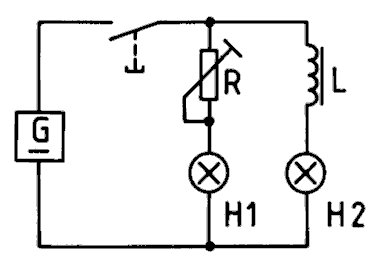
\includegraphics[scale=0.35]{Spule/Bilder/TC305.png}}%Frage
{leuchtet H1 zuerst.}%A
{leuchtet H2 zuerst.}%B
{leuchten H1 und H2 genau gleich schnell.}%C
{leuchtet H2 kurz auf und geht wieder aus. H1 leuchtet.}%D
{A}%Lösung

\mucho{9}{TC402}
{Ein Trafo liegt an 45 Volt und gibt 180 Volt ab. Seine Primärwicklung hat 150 Windungen. Wie groß ist seine Sekundärwindungszahl?}%Frage
{46 Windungen}%A
{30 Windungen}%B
{600 Windungen}%C
{850 Windungen}%D
{C: $\dfrac{N_1}{N_2} = \dfrac{U_1}{U_2}$; $N_2 = \dfrac{180V}{45V} \cdot 150$}%Lösung

\mucho{10}{TC403}
{Die Primärspule eines Übertragers hat die fünffache Anzahl von Windungen der Sekundärspule. Wie hoch ist die erwartete Sekundärspannung, wenn die Primärspule an eine 230-V-Stromversorgung angeschlossen wird?}%Frage
{46 Volt}%A
{9,2 Volt}%B
{23 Volt}%C
{1150 Volt}%D
{A: $\dfrac{N_1}{N_2} = \dfrac{U_1}{U_2}$; $U_2 = \dfrac{1}{5} \cdot 230V$}%Lösung

\mucho{11}{TC304}
{Das folgende Bild zeigt einen Kern, um den ein Kabel für den Bau einer Netzdrossel gewickelt ist. Der Kern sollte aus\\ 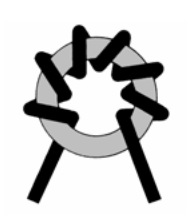
\includegraphics[scale=0.9]{Spule/Bilder/TC304.png}}%Frage
{Kunststoff bestehen.}%A
{Ferrit bestehen.}%B
{Stahl bestehen.}%C
{aus gut leitendem Material bestehen.}%D
{B}%Lösung

\mucho{12}{TC306}
{Mit zunehmender Frequenz}%Frage
{sinkt der Wechselstromwiderstand einer Spule.}%A
{sinkt der Wechselstromwiderstand einer Spule
bis zu einem Minimum und steigt dann wieder.}%B
{steigt der Wechselstromwiderstand einer Spule
bis zu einem Maximum und sinkt dann wieder.}%C
{steigt der Wechselstromwiderstand einer Spule.}%D
{D}%Lösung

%----------------------------
\newpage

\section*{Praktische Anwendung}

\subsection*{Spule wickeln}

% FIXME Foto einer eigenen Spule
\begin{wrapfigure}{r}{0.4\textwidth}
 \vspace{-10pt}
 \centering 
 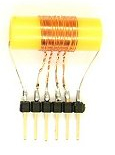
\includegraphics[scale=4]{Spule/Bilder/Spule_bau.jpg}
 %\caption{Bildunterschrift der Grafik.}
 %\label{fig:meine-Grafik}
 \vspace{-5pt}
\end{wrapfigure}

% Sollte auf Mehrband-RX hinführen - ist aber zu aufändig
% Für den ersten Versuch soll eine Spule mit insgesamt $25 $Windungen und vier
% Anzapfungen gewickelt werden. Als Wickelkörper soll eine 8 mm dickes und $3cm$
% langes Stück eines Trinkhalmes verwendet werden. Zwei Löcher im Abstand $1cm$
% helfen die Drahtenden zu fixieren. Es werden dann jeweils $5$ Windungen
% gewickelt, eine Schlaufe verdrillt und die folgenden Windungen aufgetragen. Die
% fertige Spule wird an einen Abschnitt Pfostenstecker mit sechs Kontakten
% gelötet. 

Für den ersten Versuch soll eine Spule aus $1 m$ Kupferlackdraht gewickelt
werden. Denkt daran beim Wickeln die Windungszahl zu zählen!

\begin{enumerate}
  \item Als Wickelkörper dient ein $8 mm$ dickes und $3cm$ langes Stück eines
    Trinkhalmes.
  \item Zwei Löcher im Abstand $1cm$ helfen die Drahtenden zu fixieren.
  \item Um die Kontakte der Spule frei zu legen, muss die aufgetragene
    Lackschicht abgeschabt oder mit einem Feuerzeug freigebrannt werden.
  \item Berechnet die Induktivität $L$ eurer Spule und messt mit dem
    LC-Messgerät nach.
\end{enumerate}

\loesung{Die Spule sollte um die $3-5 uH$ haben, damit der darauf aufbauende
KW-Empfänger-Versuch mit einem Schwingkreis um die $7 MHz$ klappt.}

\subsection*{Impedanz von C und L}

Wdh. Kondensator:

\begin{itemize}
    \item Erzeuge mit den Klinkenanschlusskabel und einem Signalgenerator
      Sinusschwingungen und finde heraus in welchem Bereich die Schwingungen
      noch deutlich hörbar sind.
    \item Schleife nun einen Koppelkondensator mit $C = 100 nF$ ein. Welche Unterschiede
      sind hörbar? \loesung{Hochpassverhalten}
    \item Berechne die Impedanz der Kondensators in den oberen und unteren
      Bereichen der Hörschwelle.
    \item Zusatzaufgabe: Was passiert mit einem Rechtecksignal?
\end{itemize}

% TODO Induktivität/Kapazität als Energiespeicher:
%      * siehe Experiment TC305
%      * Glimmlampen
%      * mit Dioden antiparallel?

Spule:

\begin{itemize}
  \item Wiederholt das o.g. Experiment mit eurer Spule -- was fällt euch auf?
  \item Wiederholt das o.g. Experiment noch einmal mit einer geg. Spule -- hier
    reicht das Messen der Impedanz % FIXME
\end{itemize}

\loesung{Ziel in diesem Teil ist es herauszufinden, dass es unglaubliche
Windugszahlen bei Spulen erfordert um etwas im niederfrequenten Bereich zu
erreichen.}

% DONE Spannungsteilerversuch mit 1 Ohm und Induktivität von bis zu 20 uH
%      fehlgeschlagen :-( Allein die Übergangswiderstände machen schon zu viel aus
% TODO einfaches Audiofilter als Notch?
% TODO Induktionsversuch a la Trafo?



\chapter{Der Schwingkreis}
%\begin{wrapfigure}[0]{r}[-2.5cm]{3cm}
% \vspace{-6cm}
% \includegraphics[scale=0.4]{Schwingkreis/Bilder/schwingkreis.png}
% \vspace{-6cm}
%\end{wrapfigure}

\section*{Theorie- und Prüfungsfragen} 

\mucho{1}{TD203}
{Was ist im Resonanzfall bei der Reihenschaltung einer Induktivität mit einer Kapazität erfüllt?}%Frage
{Der Betrag des induktiven Widerstands ist dann gleich dem Betrag des kapazitiven Widerstands.}%A
{Der Wert des Verlustwiderstands der Spule ist dann gleich dem Wert des Verlustwiderstands des Kondensators.}%B
{Die Größe des elektrischen Feldes in der Spule ist dann gleich der Größe des elektrischen Feldes im Kondensators.}%C
{Die Größe des magnetischen Feldes in der Spule ist dann gleich der Größe des magnetischen Feldes im Kondensator.}%D
{A}%Lösung

\mucho{2}{TD209}
{Welche Resonanzfrequenz hat die Parallelschaltung einer Spule von 2 $\mu H$ mit einem Kondensator von 60 $pF$ und einem Widerstand von 10$k\Omega$?}%Frage
{145,288kHz}%A
{1,45288MHz}%B
{14,5288MHz}%C
{145,288 MHz}%D
{C \hspace{3em} $f_0 = \frac{1}{2 \pi \sqrt{L C}}$}%Lösung

\mucho{3}{TD206}
{ Wie ändert sich die Resonanzfrequenz eines Schwingkreises, wenn
1. die Spule mehr Windungen erhält, 2. die Länge der Spule durch Zusammenschieben der Drahtwicklung verringert wird, 3. ein Kupferkern in das Innere der Spule gebracht wird?}%Frage
{Die Resonanzfrequenz wird bei 1. und 2. kleiner und bei 3. größer.}%A
{Die Resonanzfrequenz wird in allen drei Fällen kleiner.}%B
{Die Resonanzfrequenz wird bei 1. kleiner und bei 2. und 3. größer.}%C
{Die Resonanzfrequenz wird bei 1. und 2. größer und bei 3. kleiner.}%D
{A}%Lösung


\mucho{4}{TD201}
{Der Impedanzfrequenzgang in der Abbildung zeigt die Kennlinie\\ 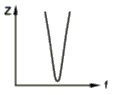
\includegraphics[scale=0.5]{Schwingkreis/Bilder/TD201.png}}%Frage
{eines Serienschwingkreises.}%A
{eines Parallelschwingkreises.}%B
{einer Induktivität.}%C
{einer Kapazität.}%D
{A}%Lösung

\vspace*{0.65cm}

\mucho{5}{TD202}
{Der Impedanzfrequenzgang in der Abbildung zeigt die Kennlinie\\
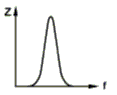
\includegraphics[scale=0.5]{Schwingkreis/Bilder/TD202.png}}%Frage
{eines Serienschwingkreises.}%A
{eines Parallelschwingkreises.}%B
{einer Induktivität.}%C
{einer Kapazität.}
{B}%Lösung

\aufgabentext{
	\begin{enumerate}
	\item[6] Um welche Schaltungen handelt es sich in folgender Abbildung.
	\end{enumerate}
	\loesung{1 Reihenschwingkreis, 2 Parallelschwingkreis, 3 Tiefpass, 4 Hochpass, 5 Bandpass, 6 Saugkreis, 7 Sperrkreis }
	}

\begin{figure}[H]
	\centering
	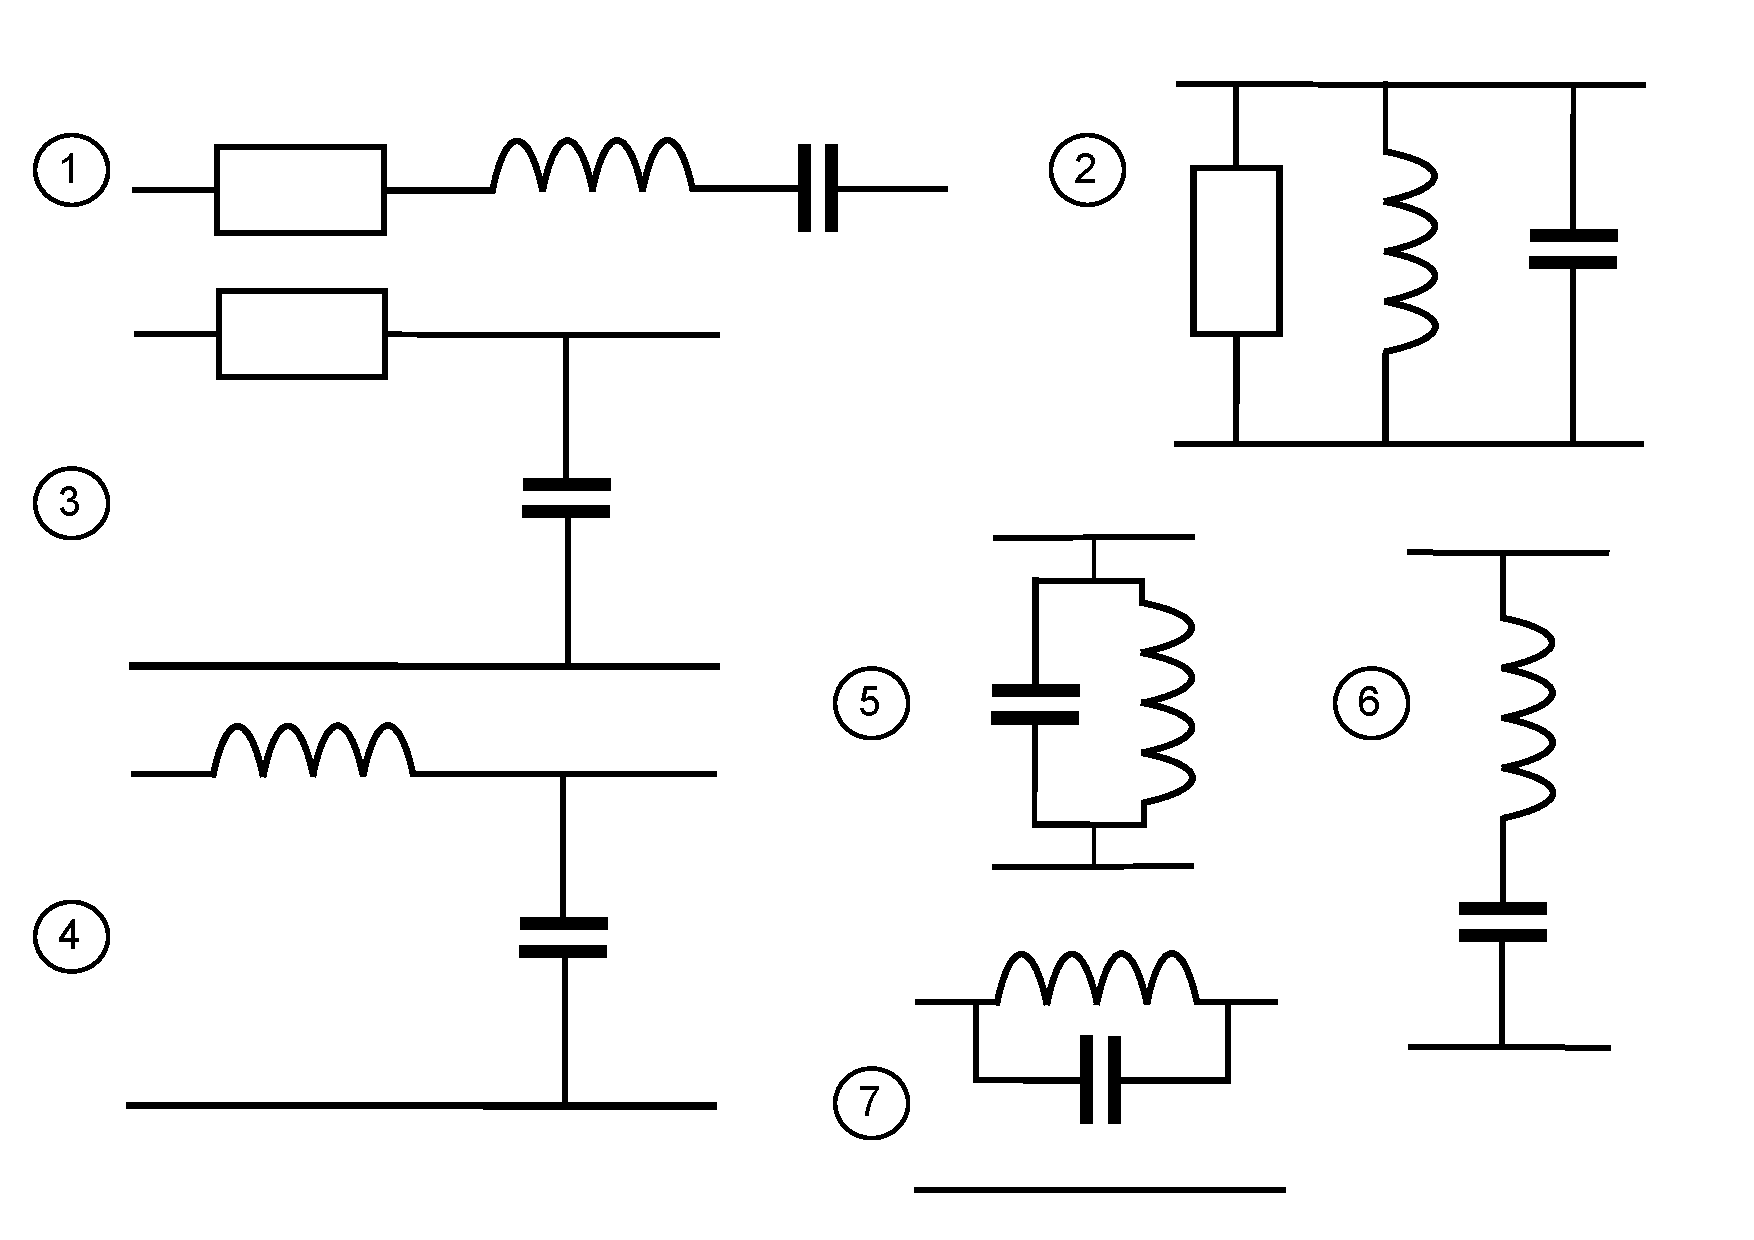
\includegraphics[scale=0.5]{Schwingkreis/Bilder/Filterschaltungen.pdf}
	\end{figure}

\mucho{7}{TD213}
{Welche Grenzfrequenz ergibt sich bei einem RC-Tiefpass mit einem Widerstand von 10$k\Omega$ und einem Kondensator von 50$nF$?}%Frage
{0,32$Hz$}%A
{318$Hz$}%B
{421$Hz$}%C
{318$kHz$}%D
{B \hspace{3em} $f_g = \frac{1}{2 \pi R C}$}%Lösung

\section*{Praxis}

\subsection*{Vorbereitung}

Seht euch die Pin-Belegung des Raspberry Pi (siehe Abbildung \ref{rpi}) sowie
die zu layoutende Schaltung für den 70cm-Tiefpassfilter (siehe Abbildung
\ref{70cmLP}) an.

\begin{figure}[H]
    \centering
    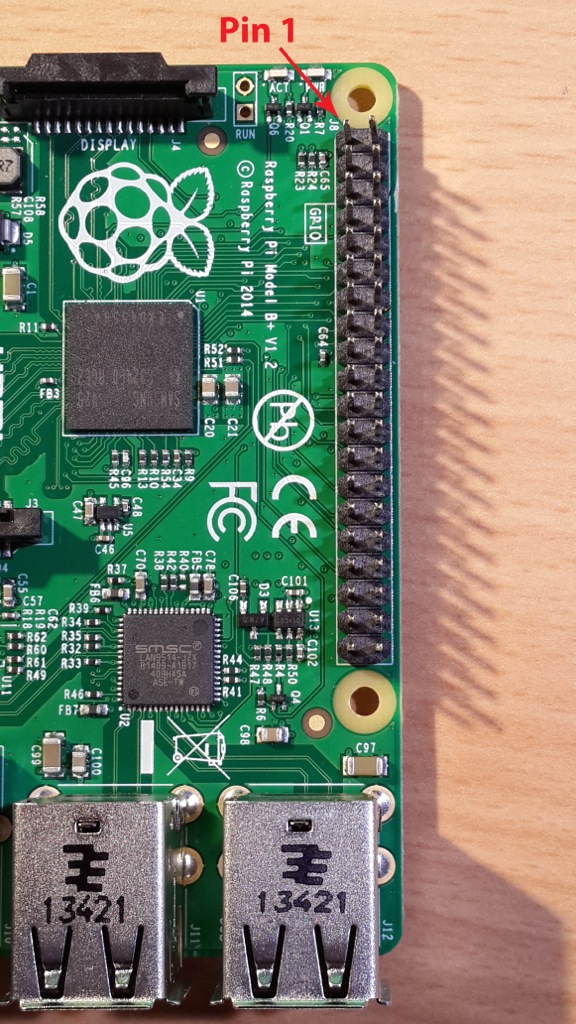
\includegraphics[height=0.4\textheight]{Schwingkreis/Bilder/B_plus_hdr_sm.jpg}
    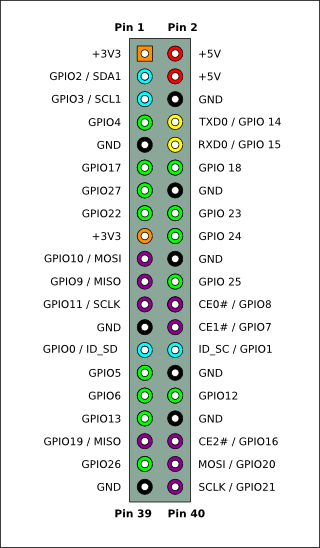
\includegraphics[height=0.4\textheight]{Schwingkreis/Bilder/Pi-GPIO-header.png}
    \caption{Connector pinout (P1 Header) -- Models B+, B2}
    \label{rpi}
    %FIXME Abbildungs-Quellenverzeichnis \url{http://elinux.org/RPi_Low-level_peripherals#Model_A.2B.2C_B.2B_and_B2}
\end{figure}

\begin{figure}[H]
    \centering
    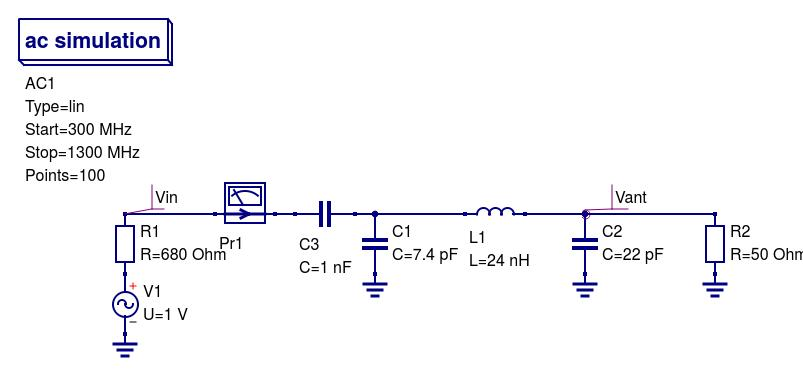
\includegraphics[width=1\textwidth]{Schwingkreis/Bilder/70cmLP500Ohm.jpg}
    \caption{Schaltung des 70cm-Tiefpassfilters aus Qucs}
    \label{70cmLP}
\end{figure}

\subsection*{Fritzing}

\subsubsection{Schematic View}

Bauteile aus den \emph{Core Parts} hinzufügen:

\begin{itemize}
    \item  Basic
    \begin{itemize}
        \item Resistor $680 \Omega$ (THT)
        \item Inductor $22 nH$ (SMD 1206)
        \item Ceramic Capacitor $1 nF$ (THT)
        \item Ceramic Capacitor $22 pF$ (THT)
    \end{itemize}
    \item  Input
    \begin{itemize}
        \item Variable Capacitor $2.1-10 pF$ (THT, $3.81mm$ pin spacing)
        \item Antenna (Wire soldering point)
    \end{itemize}
    \item Connection
    \begin{itemize}
        \item Generic female header (THT, 2x10, flip horizontal)
    \end{itemize}
    \item Schematic View
    \begin{itemize}
        \item Ground
    \end{itemize}
\end{itemize}

Nun können die Bauteile entsprechend des Schaltplanes verdrahtet werden.
\textbf{Hinweis}: Die Pin-Zählung des \emph{Generic female header} stimmt nicht
mit der des Raspberry Pi überein.

\begin{itemize}
    \item GPIO = Pin 16
    \item GND = Pin 17
\end{itemize}

\subsubsection{PCB View}

\begin{itemize}
    \item PCB ändern auf One Layer \& Fäche ca. $30x30mm$
    \item Bauteile anordnen (THT-Bauteile auf Vorderseite, SMD auf Unterseite)
    \item Leitungen ziehen
    \item optional: Copper Fill Blocker \& Silkscreen Text
    \item Rechtsklick auf einen Ground Pin: "`Set Ground Fill Seed"'
    \item Menü $\rightarrow$ Routing $\rightarrow$ Ground Fill
\end{itemize}

\subsubsection{Zusatzaufgaben}

\begin{itemize}
    \item Antennenanschluss auf folgende MCX-Buchse umbauen: \\
          \url{http://www.reichelt.de/index.html?ARTICLE=152523}
    \item Testboard mit verschiedenen PCB-Spulen um ~24 nH erstellen, da typ. 2-3\% Abweichung. \\
          Berechnungsgrundlagen mit Online calculator:\\
          \url{http://coil32.net/pcb-coil.html}\\
          alternative Formen: \\
          \url{http://www.circuits.dk/calculator_planar_coil_inductor.htm}
\end{itemize}


\chapter{Die Diode}


\begin{wrapfigure}[0]{r}[-2cm]{4cm}
 \vspace{-5cm}
 %\centering 
 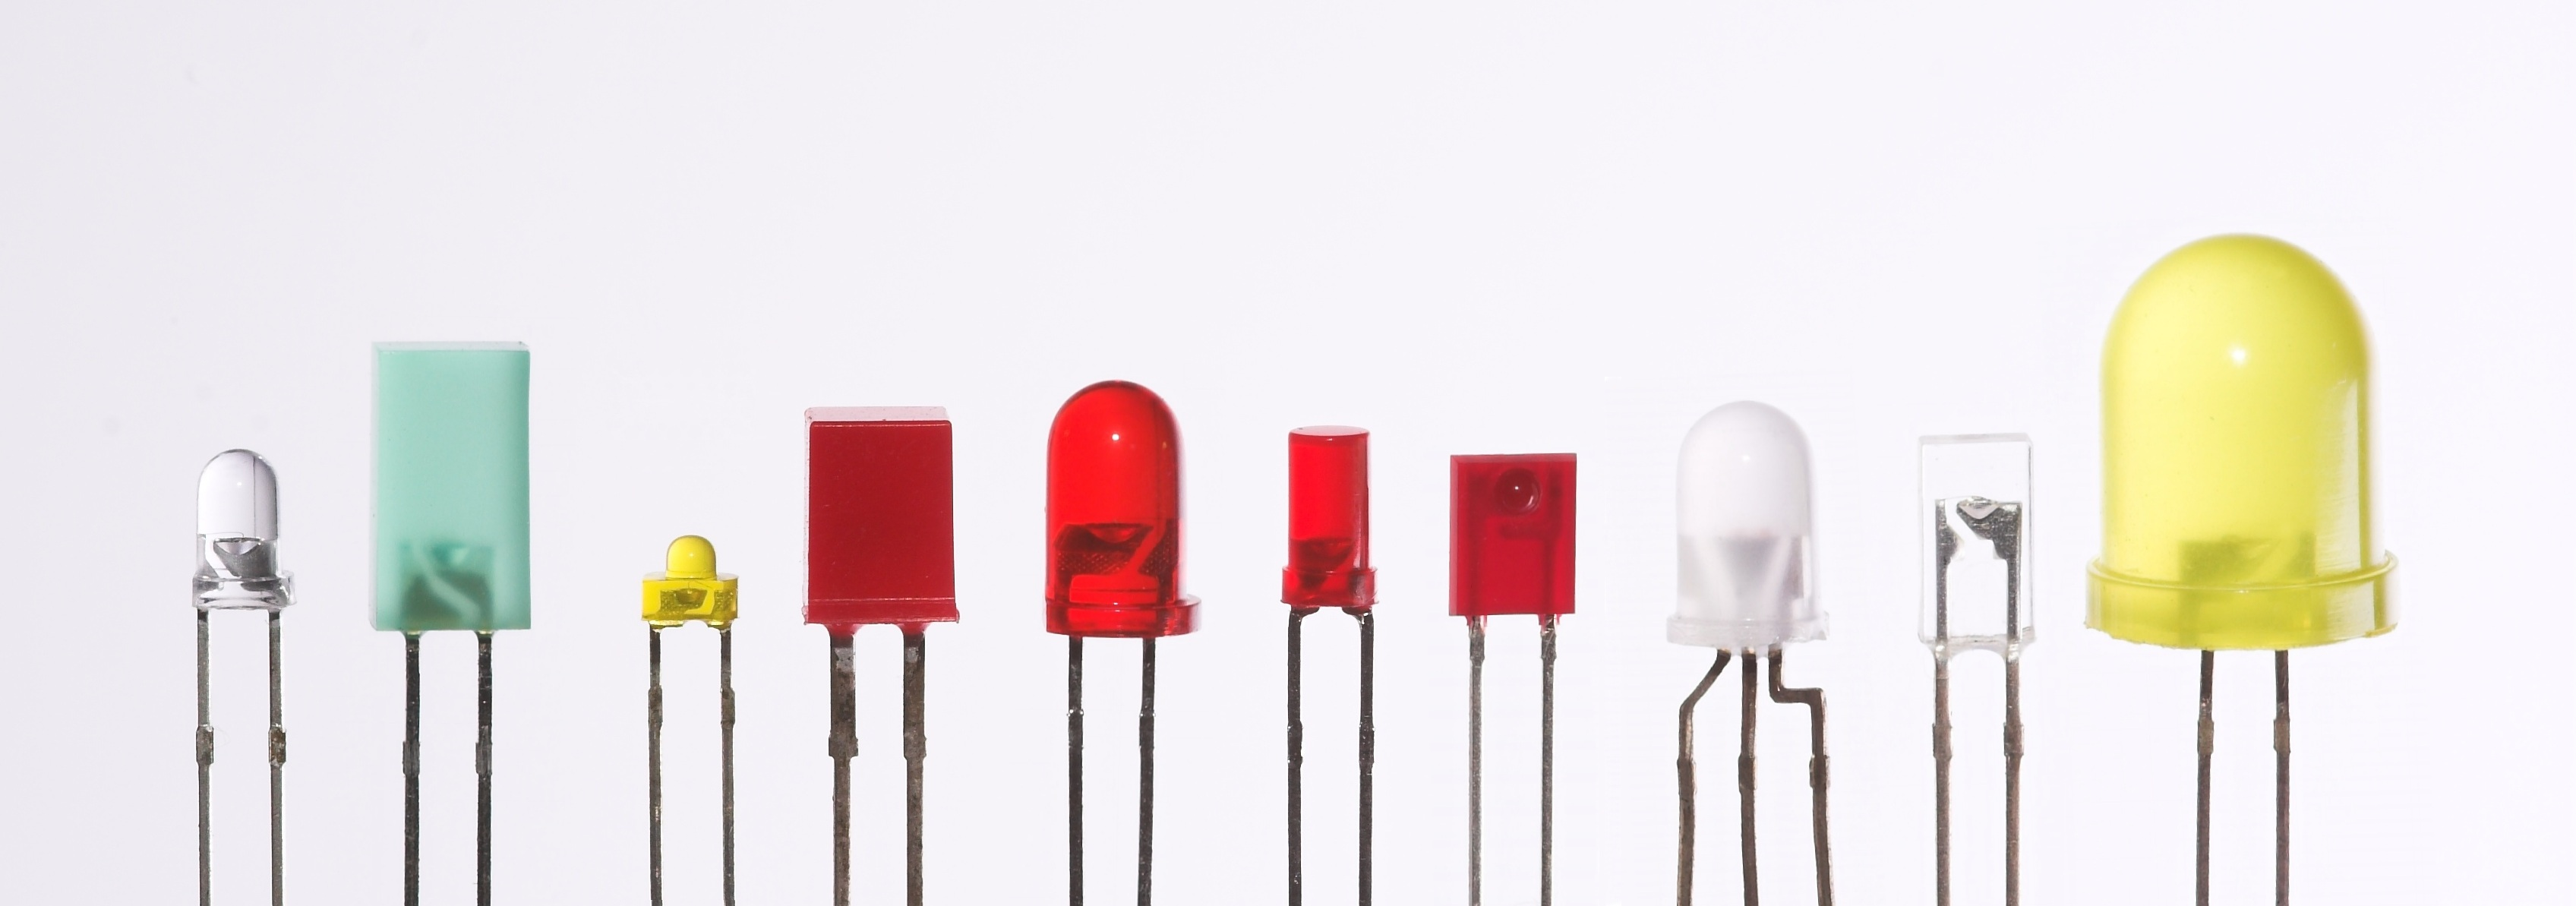
\includegraphics[scale=0.25]{Diode/Bilder/Verschiedene_LEDs.jpg}
 %\caption{Bildunterschrift der Grafik.}
 %\label{fig:meine-Grafik}
 \vspace*{-5cm}
\end{wrapfigure}


\section*{Theorie- und Prüfungsfragen} 

\subsection*{Dotierung}

\begin{enumerate}
	\itemsep1pt\parskip0pt\parsep0pt
	\item[1] Was bedeutet der Begriff Dotierung?
        \loesung{\textbf{Dotierung} bezeichnet in der Halbleitertechnik das
        einbringen von Fremdatomen in ein Grundmaterial zur Veränderung der
        elektrischen Leitfähigkeit.}
\end{enumerate}

\begin{enumerate}
\item[2] \emph{\textbf{TB105}}    Was verstehen Sie unter Halbleitermaterialien? Einige Stoffe wie z.B. ...
	\begin{enumerate}
	\itemsep1pt\parskip0pt\parsep0pt
		\item[A] Silizium, Germanium sind in reinem Zustand gute Isolatoren. Durch geringfügige Zusätze von geeigneten anderen Stoffen werden sie jedoch zu Leitern.
		\item[B] Silizium, Germanium sind in reinem Zustand gute Isolatoren. Durch geringfügige Zusätze von geeigneten anderen Stoffen nimmt jedoch ihre Leitfähigkeit ab.
		\item[C]  Indium oder Magnesium sind in reinem Zustand gute Isolatoren. Durch geringfügige Zusätze von geeigneten anderen Stoffen werden sie jedoch zu Leitern.
		\item[D] Silizium, Germanium sind in trockenem Zustand gute Elektrolyten. Durch geringfügige Zusätze von Wismut oder Tellur kann man daraus entweder N-leitendes oder P-leitendes Material für Anoden bzw. Katoden von Halbleiterbauelementen herstellen.
		\loesung{Lösung A}
	\end{enumerate}
\end{enumerate}

\begin{enumerate}
\item[3] \emph{\textbf{TC501}}    P-dotiertes Halbleitermaterial ist solches, das mit einem zusätzlichen Stoff versehen wurde, der
	\begin{enumerate}
	\itemsep1pt\parskip0pt\parsep0pt
		\item[A] mehr als vier Valenzelektronen enthält.
		\item[B] genau vier Valenzelektronen enthält.
		\item[C] weniger als vier Valenzelektronen enthält.
		\item[D] keine Valenzelektronen enthält.
		 \loesung{Lösung C}
	\end{enumerate}
\end{enumerate}


\begin{enumerate}
\item[4] \emph{\textbf{TC502}}   N-leitendes Halbleitermaterial ist gekennzeichnet durch
	\begin{enumerate}
	\itemsep1pt\parskip0pt\parsep0pt
		\item[A] Überschuss an freien Elektronen.
		\item[B] das Fehlen von Dotierungsatomen.
		\item[C] das Fehlen von Atomen im Gitter des Halbleiterkristalls.
		\item[D] bewegliche Elektronenlücken.
		\loesung{Lösung A}
	\end{enumerate}
\end{enumerate}


\begin{enumerate}
\item[5] \emph{\textbf{TC503}}  Ein in Durchlassrichtung betriebener PN-Übergang ermöglicht
	\begin{enumerate}
	\itemsep1pt\parskip0pt\parsep0pt
		\item[A] den Stromfluss von N nach P.
		\item[B] den Stromfluss von P nach N.
		\item[C] keinen Stromfluss.
		\item[D] den Elektronenfluss von P nach N.
		\loesung{Lösung B}
	\end{enumerate}
\end{enumerate}


\subsection*{Die Diode}

\begin{enumerate}
\itemsep1pt\parskip0pt\parsep0pt
\item[6] Skizziere das Schaltzeichen einer Diode und markiere die Anode, die Kathode und die jeweilige Dotierung.
    \loesung{
    \begin{figure}[H]
    \centering 
    % Graphic for TeX using PGF
% Title: /home/stole/Dokumente/git/afutub-kurs/Praxisskript/Diode/Schaltungen/Diode.dia
% Creator: Dia v0.97.3
% CreationDate: Mon Nov 16 20:36:17 2015
% For: stole
% \usepackage{tikz}
% The following commands are not supported in PSTricks at present
% We define them conditionally, so when they are implemented,
% this pgf file will use them.
\ifx\du\undefined
  \newlength{\du}
\fi
\setlength{\du}{15\unitlength}
\begin{tikzpicture}
\pgftransformxscale{1.000000}
\pgftransformyscale{-1.000000}
\definecolor{dialinecolor}{rgb}{0.000000, 0.000000, 0.000000}
\pgfsetstrokecolor{dialinecolor}
\definecolor{dialinecolor}{rgb}{1.000000, 1.000000, 1.000000}
\pgfsetfillcolor{dialinecolor}
\pgfsetlinewidth{0.100000\du}
\pgfsetdash{}{0pt}
\pgfsetdash{}{0pt}
\pgfsetbuttcap
\pgfsetmiterjoin
\pgfsetbuttcap
\pgfsetmiterjoin
\pgfsetdash{}{0pt}
\definecolor{dialinecolor}{rgb}{0.000000, 0.000000, 0.000000}
\pgfsetstrokecolor{dialinecolor}
\draw (15.422302\du,-15.899999\du)--(15.422302\du,-13.022298\du);
\pgfsetbuttcap
\pgfsetmiterjoin
\pgfsetdash{}{0pt}
\definecolor{dialinecolor}{rgb}{0.000000, 0.000000, 0.000000}
\pgfsetstrokecolor{dialinecolor}
\draw (15.422302\du,-13.022298\du)--(18.300002\du,-14.461149\du);
\pgfsetbuttcap
\pgfsetmiterjoin
\pgfsetdash{}{0pt}
\definecolor{dialinecolor}{rgb}{0.000000, 0.000000, 0.000000}
\pgfsetstrokecolor{dialinecolor}
\draw (15.422302\du,-15.899999\du)--(18.300002\du,-14.461149\du);
\pgfsetbuttcap
\pgfsetmiterjoin
\pgfsetdash{}{0pt}
\definecolor{dialinecolor}{rgb}{0.000000, 0.000000, 0.000000}
\pgfsetstrokecolor{dialinecolor}
\draw (15.422302\du,-14.461149\du)--(18.300002\du,-14.461149\du);
\pgfsetbuttcap
\pgfsetmiterjoin
\pgfsetdash{}{0pt}
\definecolor{dialinecolor}{rgb}{0.000000, 0.000000, 0.000000}
\pgfsetstrokecolor{dialinecolor}
\draw (18.300002\du,-15.899999\du)--(18.300002\du,-13.022298\du);
\pgfsetlinewidth{0.100000\du}
\pgfsetdash{}{0pt}
\pgfsetdash{}{0pt}
\pgfsetbuttcap
{
\definecolor{dialinecolor}{rgb}{0.000000, 0.000000, 0.000000}
\pgfsetfillcolor{dialinecolor}
% was here!!!
\definecolor{dialinecolor}{rgb}{0.000000, 0.000000, 0.000000}
\pgfsetstrokecolor{dialinecolor}
\draw (18.300002\du,-14.461149\du)--(21.040301\du,-14.459230\du);
}
\pgfsetlinewidth{0.100000\du}
\pgfsetdash{}{0pt}
\pgfsetdash{}{0pt}
\pgfsetbuttcap
{
\definecolor{dialinecolor}{rgb}{0.000000, 0.000000, 0.000000}
\pgfsetfillcolor{dialinecolor}
% was here!!!
\definecolor{dialinecolor}{rgb}{0.000000, 0.000000, 0.000000}
\pgfsetstrokecolor{dialinecolor}
\draw (12.987653\du,-14.460276\du)--(15.422302\du,-14.461149\du);
}
% setfont left to latex
\definecolor{dialinecolor}{rgb}{0.000000, 0.000000, 0.000000}
\pgfsetstrokecolor{dialinecolor}
\node[anchor=west] at (11.448825\du,-14.995418\du){Anode};
% setfont left to latex
\definecolor{dialinecolor}{rgb}{0.000000, 0.000000, 0.000000}
\pgfsetstrokecolor{dialinecolor}
\node[anchor=west] at (19.327825\du,-14.872736\du){Kathode};
\pgfsetlinewidth{0.100000\du}
\pgfsetdash{}{0pt}
\pgfsetdash{}{0pt}
\pgfsetmiterjoin
\definecolor{dialinecolor}{rgb}{1.000000, 1.000000, 1.000000}
\pgfsetfillcolor{dialinecolor}
\fill (14.976770\du,-11.192971\du)--(14.976770\du,-7.792972\du)--(18.376770\du,-7.792972\du)--(18.376770\du,-11.192971\du)--cycle;
\definecolor{dialinecolor}{rgb}{0.000000, 0.000000, 0.000000}
\pgfsetstrokecolor{dialinecolor}
\draw (14.976770\du,-11.192971\du)--(14.976770\du,-7.792972\du)--(18.376770\du,-7.792972\du)--(18.376770\du,-11.192971\du)--cycle;
\pgfsetlinewidth{0.100000\du}
\pgfsetdash{}{0pt}
\pgfsetdash{}{0pt}
\pgfsetmiterjoin
\definecolor{dialinecolor}{rgb}{1.000000, 1.000000, 1.000000}
\pgfsetfillcolor{dialinecolor}
\fill (18.376770\du,-11.192970\du)--(18.376770\du,-7.792971\du)--(21.776770\du,-7.792971\du)--(21.776770\du,-11.192970\du)--cycle;
\definecolor{dialinecolor}{rgb}{0.000000, 0.000000, 0.000000}
\pgfsetstrokecolor{dialinecolor}
\draw (18.376770\du,-11.192970\du)--(18.376770\du,-7.792971\du)--(21.776770\du,-7.792971\du)--(21.776770\du,-11.192970\du)--cycle;
\pgfsetlinewidth{0.100000\du}
\pgfsetdash{}{0pt}
\pgfsetdash{}{0pt}
\pgfsetbuttcap
{
\definecolor{dialinecolor}{rgb}{0.000000, 0.000000, 0.000000}
\pgfsetfillcolor{dialinecolor}
% was here!!!
\definecolor{dialinecolor}{rgb}{0.000000, 0.000000, 0.000000}
\pgfsetstrokecolor{dialinecolor}
\draw (13.176770\du,-9.492971\du)--(14.976770\du,-9.492972\du);
}
\pgfsetlinewidth{0.100000\du}
\pgfsetdash{}{0pt}
\pgfsetdash{}{0pt}
\pgfsetmiterjoin
\definecolor{dialinecolor}{rgb}{0.000000, 0.000000, 0.000000}
\pgfsetfillcolor{dialinecolor}
\fill (14.976770\du,-11.192971\du)--(14.976770\du,-7.778107\du)--(15.911899\du,-7.778107\du)--(15.911899\du,-11.192971\du)--cycle;
\definecolor{dialinecolor}{rgb}{0.000000, 0.000000, 0.000000}
\pgfsetstrokecolor{dialinecolor}
\draw (14.976770\du,-11.192971\du)--(14.976770\du,-7.778107\du)--(15.911899\du,-7.778107\du)--(15.911899\du,-11.192971\du)--cycle;
\pgfsetlinewidth{0.100000\du}
\pgfsetdash{}{0pt}
\pgfsetdash{}{0pt}
\pgfsetmiterjoin
\definecolor{dialinecolor}{rgb}{0.000000, 0.000000, 0.000000}
\pgfsetfillcolor{dialinecolor}
\fill (20.776770\du,-11.192971\du)--(20.776770\du,-7.792971\du)--(21.776770\du,-7.792971\du)--(21.776770\du,-11.192971\du)--cycle;
\definecolor{dialinecolor}{rgb}{0.000000, 0.000000, 0.000000}
\pgfsetstrokecolor{dialinecolor}
\draw (20.776770\du,-11.192971\du)--(20.776770\du,-7.792971\du)--(21.776770\du,-7.792971\du)--(21.776770\du,-11.192971\du)--cycle;
% setfont left to latex
\definecolor{dialinecolor}{rgb}{0.000000, 0.000000, 0.000000}
\pgfsetstrokecolor{dialinecolor}
\node[anchor=west] at (13.476772\du,-11.692970\du){p-dotiert};
% setfont left to latex
\definecolor{dialinecolor}{rgb}{0.000000, 0.000000, 0.000000}
\pgfsetstrokecolor{dialinecolor}
\node[anchor=west] at (20.476772\du,-11.692970\du){n-dotiert};
\pgfsetlinewidth{0.100000\du}
\pgfsetdash{}{0pt}
\pgfsetdash{}{0pt}
\pgfsetbuttcap
{
\definecolor{dialinecolor}{rgb}{0.000000, 0.000000, 0.000000}
\pgfsetfillcolor{dialinecolor}
% was here!!!
\definecolor{dialinecolor}{rgb}{0.000000, 0.000000, 0.000000}
\pgfsetstrokecolor{dialinecolor}
\draw (21.776770\du,-9.492971\du)--(23.565624\du,-9.475251\du);
}
\end{tikzpicture}

    \end{figure}
    }
\item[7] Skizziere die Strom-Spannungskennlinie und markieren den Durchlassbereich, den Sperrbereich und den Durchbruchbereich.
	\loesung{
	\begin{figure}[H]
    \centering 
    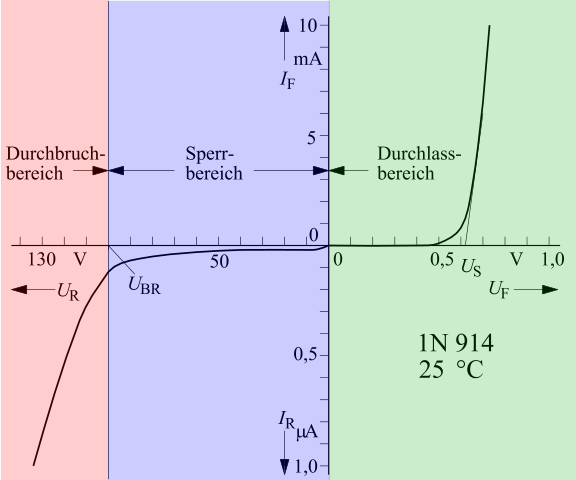
\includegraphics[scale=0.5]{Diode/Bilder/Kennlinie_Diode.png}
    \end{figure}
    }
\end{enumerate}

\mucho{8}{TC504}
{Eine in Sperrrichtung betriebene Diode hat}%Frage
{einen hohen Widerstand.}%A
{eine hohe Kapazität.}%B
{eine geringe Impedanz.}%C
{eine hohe Induktivität.}%D
{A}%Lösung

\mucho{9}{TC508}
{Wozu dient die folgende Schaltung?\\ 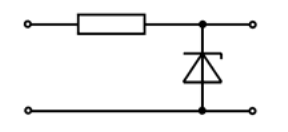
\includegraphics[scale=0.63]{Diode/Bilder/TC508.png}}%Frage
{zur Signalbegrenzung.}%A
{zur Spannungsstabilisierung.}%B
{als Leuchtanzeige.}%C
{zur Stromgewinnung.}%D
{B}%Lösung

\mucho{10}{TC505}
{Die Auswahlantworten enthalten Silizium-Dioden mit unterschiedlichen Arbeitspunkten. Bei welcher Antwort befindet sich die Diode in leitendem Zustand?}%Frage
{$-2,6V $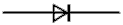
\includegraphics[scale=0.5]{Diode/Bilder/Diode_r.png} $-2,0V$}%A
{$~~~~15V$ 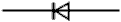
\includegraphics[scale=0.5]{Diode/Bilder/Diode_l.png} $~~~9V$}%B
{$~~0,7V$ 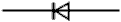
\includegraphics[scale=0.5]{Diode/Bilder/Diode_l.png} $1,3V$}%C
{$~~3,4V$ 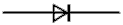
\includegraphics[scale=0.5]{Diode/Bilder/Diode_r.png} $4,0V$}%D
{C}%Lösung

\mucho{11}{TC506}
{Die Auswahlantworten enthalten Silizium-Dioden mit unterschiedlichen Arbeitspunkten. Bei welcher Antwort befindet sich die Diode in leitendem Zustand?}%Frage
{$~~5,3V $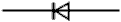
\includegraphics[scale=0.5]{Diode/Bilder/Diode_l.png} $4,7V$}%A
{$~~15V$ 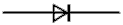
\includegraphics[scale=0.5]{Diode/Bilder/Diode_r.png} $18V$}%B
{$3,9V$ 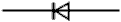
\includegraphics[scale=0.5]{Diode/Bilder/Diode_l.png} $3,2V$}%C
{$-2V$ 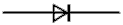
\includegraphics[scale=0.5]{Diode/Bilder/Diode_r.png} $-2,6V$}%D
{D}%Lösung

\mucho{12}{TC509}
{Wozu dient die folgende Schaltung?\\ 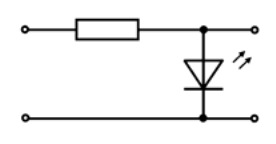
\includegraphics[scale=0.63]{Diode/Bilder/TC509.png}}%Frage
{zur Signalbegrenzung.}%A
{als Leuchtanzeige.}%B
{zur Stromgewinnung.}%C
{zur Spannungsstabilisierung.}%D
{B}%Lösung

\mucho{13}{TC507}
{Wie verhält sich die Kapazität einer Kapazitätsdiode (Varicap)?}%Frage
{Sie nimmt mit abnehmender Sperrspannung zu.}%A
{Sie erhöht sich mit zunehmender Durchlassspannung.}%B
{Sie nimmt mit zunehmender Sperrspannung zu.}%C
{Sie erhöht sich mit zunehmendem Durchlassstrom.}%D
{B}%Lösung


\chapter{Der Transistor}


\begin{wrapfigure}[2]{r}[-1cm]{4cm}
 \vspace{-6cm}
  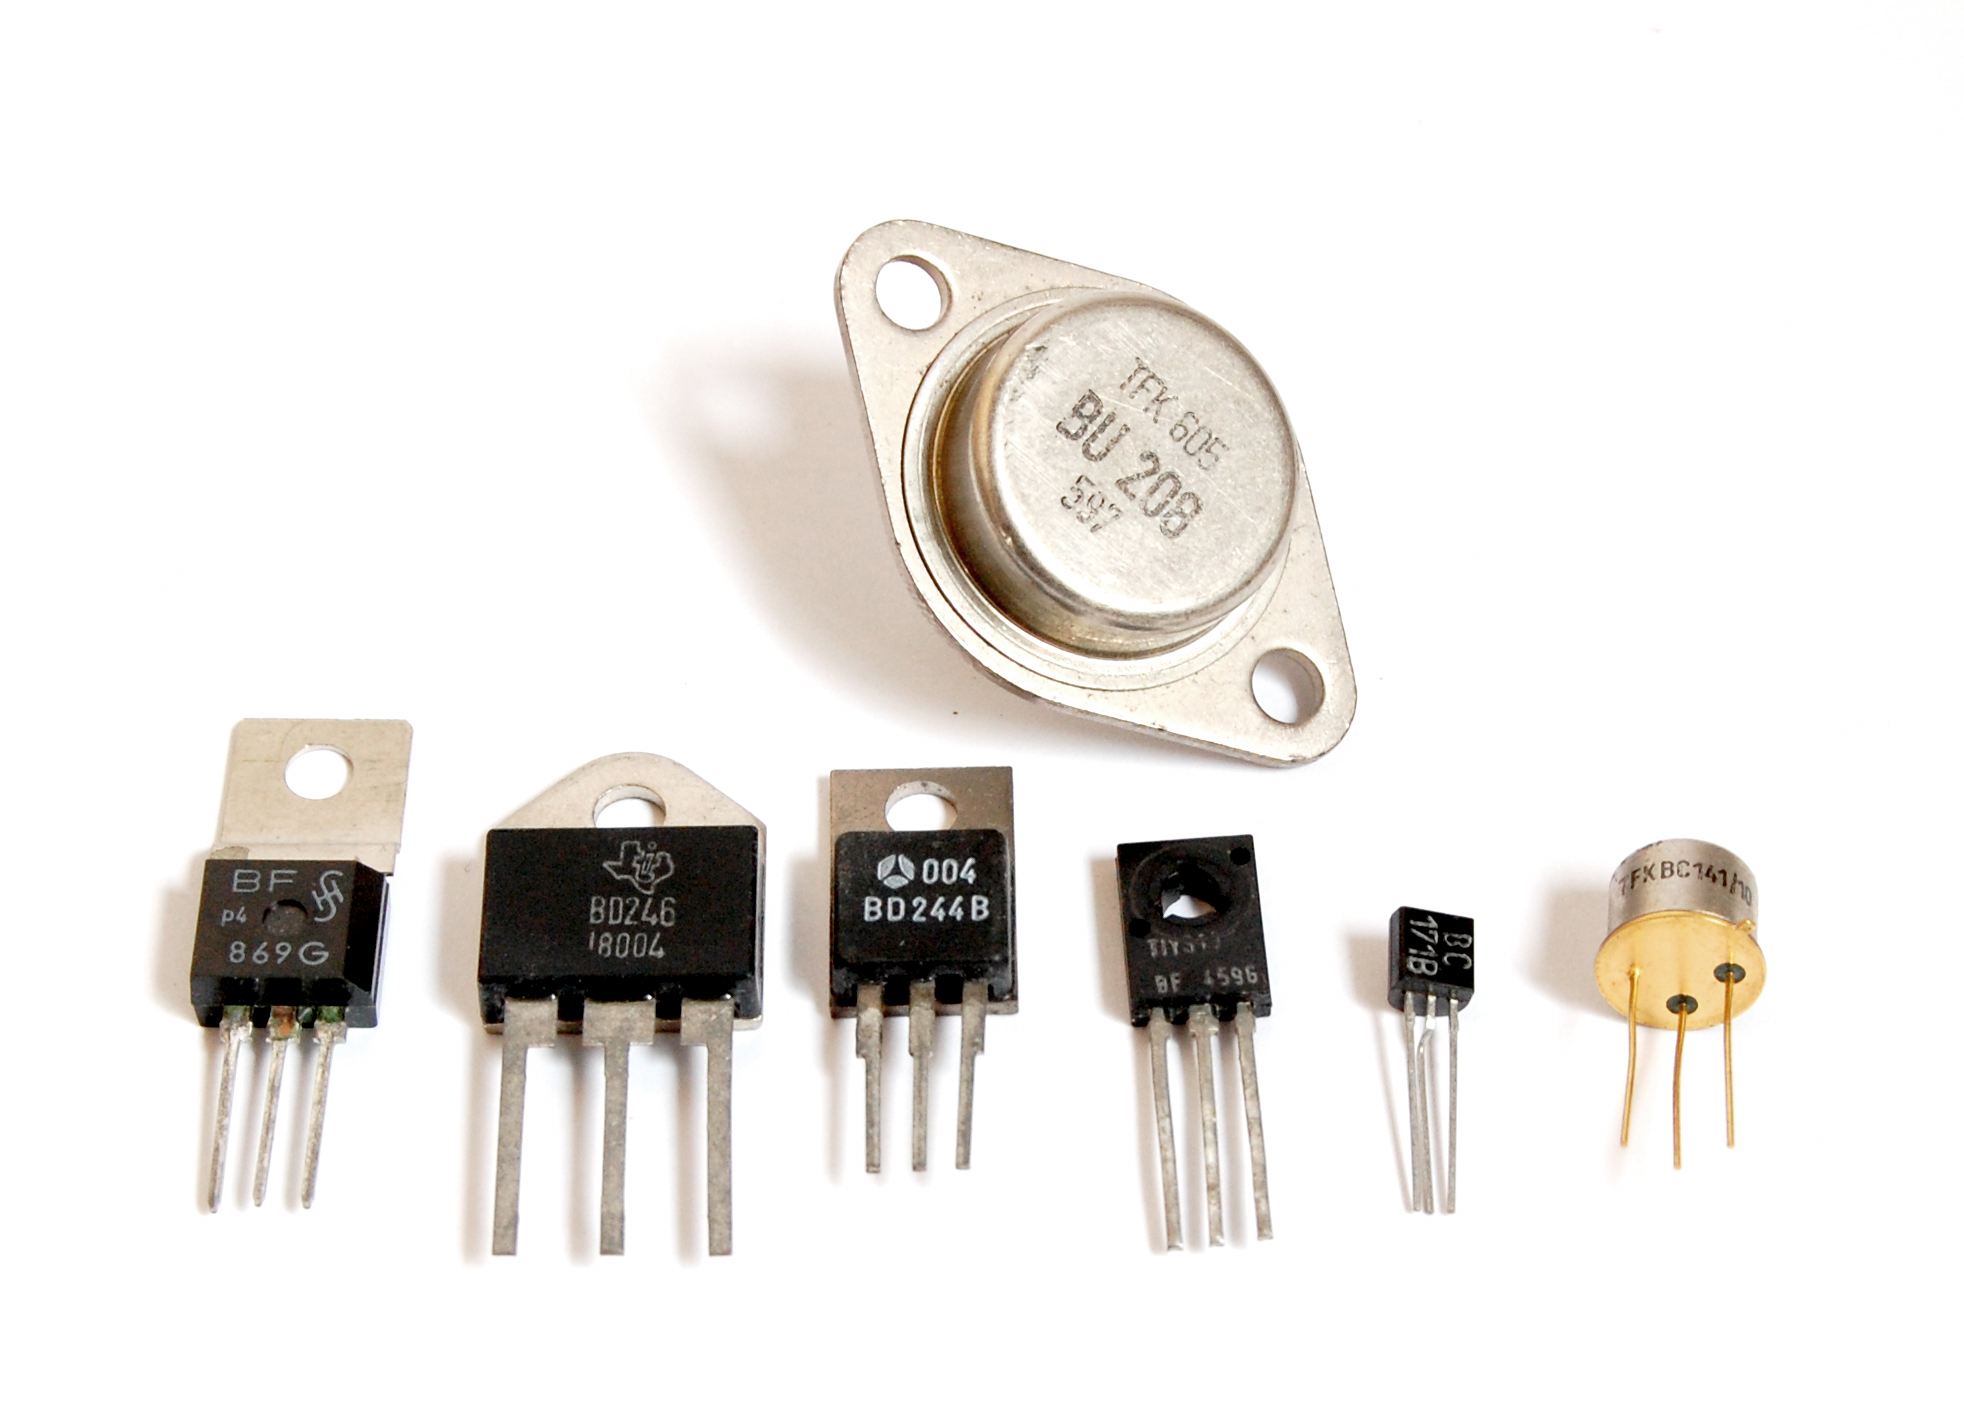
\includegraphics[scale=0.4]{Transistor/Bilder/Transistors-white.jpg}
 \vspace{-6cm}
\end{wrapfigure}

\section{Theorie- und Prüfungsfragen}

~~~~~~

\begin{enumerate}
\itemsep1pt\parskip0pt\parsep0pt
\item[i] Skizzieren Sie die Schaltzeichen eines NPN- und eines PNP-Transistors. Beschriften Sie entsprechend die Anschlüsse.
\item[ii] Zeichnen Sie das Ersatzschaltbild aus zwei Dioden für den NPN- und den PNP-Transistor.
\end{enumerate}

\begin{enumerate} 
\item[iii] \emph{\textbf{TC605}} Welche Kollektorspannungen haben NPN- und PNP-Transistoren?
	\begin{enumerate}
	\itemsep1pt\parskip0pt\parsep0pt
		\item[a] NPN- und PNP-Transistoren benötigen negative Kollektorspannungen.
		\item[b] PNP-Transistoren benötigen positive, NPN-Transistoren negative Kollektorspannung.
		\item[c] PNP- und NPN-Transistoren benötigen positive Kollektorspannungen.
		\item[d] NPN-Transistoren benötigen positive, PNP-Transistoren negative Kollektorspannungen.
	\end{enumerate}
\end{enumerate}

\loesung{	
	iii d
}

\begin{enumerate} 
\item[iv] \emph{\textbf{TC602}}  Das Verhältnis von Kollektorstrom zum Basisstrom eines Transistors liegt üblicherweise im Bereich von
	\begin{enumerate}
	\itemsep1pt\parskip0pt\parsep0pt
		\item[a] 1 zu 50 bis 1 zu 100.
		\item[b] 10 zu 1 bis 900 zu 1.
		\item[c] 1000 zu 1 bis 5000 zu 1.
		\item[d] 1 zu 100 bis 1 zu 500.
	\end{enumerate}
\end{enumerate}

\loesung{	
	iv b
}

\section{Praktische Anwendung}

\subsection[Der Bipolar-Transistor als Schalter]{Transistorschaltung 01 - Der Bipolar-Transistor als Schalter}

\begin{itemize}
\itemsep1pt\parskip0pt\parsep0pt
\item Schauen Sie sich den Bipolar-Transistor als Bauteil an und ordnen Sie die Bezeichnungen Kollektor, Basis und Emitter den einzelnen Beinchen zu.
\item Bauen Sie folgende Transistor-Schaltung auf (Abbildung \ref{s01}). 
\item Legen Sie die Versorgungsspannung an die Schaltung an.
\item Entfernen Sie unter Last die Leuchtdiode 1. Welche Auswirkungen hat das auf die Schaltung und warum?
\item \textbf{Zusatz:} Ersetzen Sie die Led durch einen Lautsprecher? Was passiert und warum?
\end{itemize}

\begin{figure}[H]
	\centering
	\subfigure[Schaltplan]{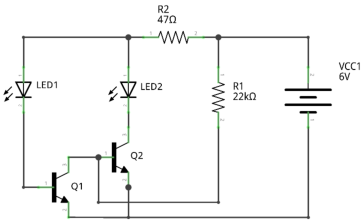
\includegraphics[scale=1.4]{Transistor/Schaltungen/NotBeleuchtung_Schaltplan.pdf}}
	\subfigure[Mögliche Breadboard-Ansicht]{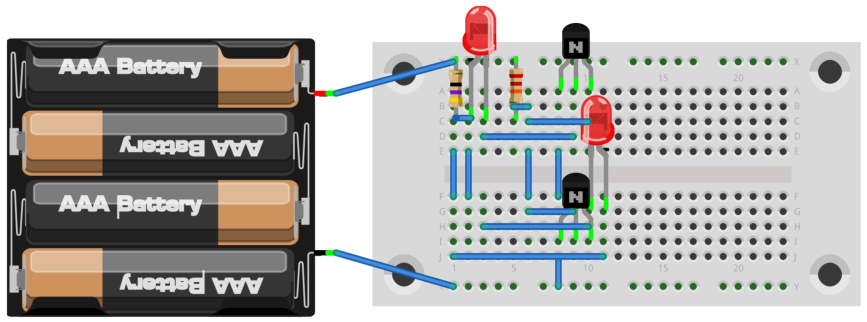
\includegraphics[scale=1]{Transistor/Schaltungen/NotBeleuchtung_Steckplatine.pdf}}
	\caption{Transistorschaltung 01 - Der Bipolar-Transistor als Schalter}
	\label{s01}
\end{figure}

%----------------------------------------------

\subsection[Der Bipolar-Transistor als Sensor]{Transistorschaltung 02 - Der Bipolar-Transistor als Sensor}

\begin{itemize}
\itemsep1pt\parskip0pt\parsep0pt
\item Bauen Sie folgende Transistor-Schaltung auf (Abbildung \ref{s02}). 
\item Legen Sie die Versorgungsspannung an die Schaltung an.
\item Berühren Sie die Basis des Transistors Q1 mit dem Finger. Was passiert und warum?
\end{itemize}

\begin{figure}[H]
	\centering
	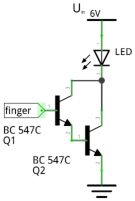
\includegraphics[scale=1.6]{Transistor/Schaltungen/NPN_Sensor.pdf}
	\caption{Transistorschaltung 02 - Der Bipolar-Transistor als Sensor}
	\label{s02}
\end{figure}

%----------------------------------------------

\subsection[Der Bipolar-Transistor als Verstärker]{Transistorschaltung 03 - Der Bipolar-Transistor als Verstärker}

\begin{itemize}
\itemsep1pt\parskip0pt\parsep0pt
\item Bauen Sie folgende Transistor-Schaltung auf (Abbildung \ref{s03}). 
\item Legen Sie die Versorgungsspannung an die Schaltung an.
\item Legen Sie ein Audiosignal an den Eingang der Schaltung an. Was passiert und warum?
\end{itemize}

\begin{figure}[H]
	\centering
	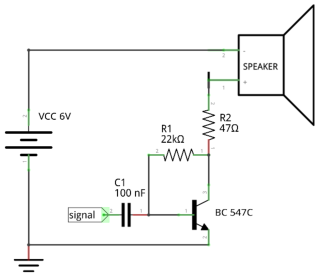
\includegraphics[scale=1.6]{Transistor/Schaltungen/NPN_Verstaerker.pdf}
	\caption{Transistorschaltung 03 - Der Bipolar-Transistor als Sensor}
	\label{s03}
\end{figure}

\newpage \vspace*{5cm}
\newpage

\chapter{Das Elektromagnetische Feld}
\begin{wrapfigure}[0]{r}[1cm]{5cm}
 \vspace{-7cm}
  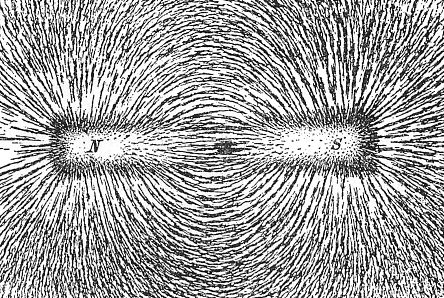
\includegraphics[scale=0.35]{Felder/Bilder/Magnet.jpg}
 \vspace{-7cm}
\end{wrapfigure}

\section*{Theorie- und Prüfungsfragen}


\begin{enumerate} 
\itemsep1pt\parskip0pt\parsep0pt
\item[1] \emph{\textbf{TB301}} Welche Einheit wird für die elektrische Feldstärke verwendet?
	\begin{enumerate}
	\itemsep1pt\parskip0pt\parsep0pt
		\item[A] Watt pro Quadratmeter $(W/m^2)$
		\item[B] Ampere pro Meter $(A/m)$
		\item[C] Henry pro Meter $(H/m)$
		\item[D] Volt pro Meter $(V/m)$
		\loesung{Lösung D}
	\end{enumerate}
\end{enumerate}

\begin{enumerate} 
\itemsep1pt\parskip0pt\parsep0pt
\item[2] Berechne das elektrische Feld eines 9V-Blockes mit $U = 9V$ und einem Klemmenabstand von $12,7mm$.
\loesung{Lösung $708,66V/m$; $E=\dfrac{U}{d}$}
\end{enumerate}

\begin{enumerate} 
\itemsep1pt\parskip0pt\parsep0pt
\item[3] \emph{\textbf{TB401}} Welche Einheit wird für die magnetische Feldstärke verwendet?
	\begin{enumerate}
	\itemsep1pt\parskip0pt\parsep0pt
		\item[A] Watt pro Quadratmeter $(W/m^2)$
		\item[B] Volt pro Meter $(V/m)$
		\item[C] Ampere pro Meter $(A/m)$
		\item[D] Henry pro Meter $(H/m)$
		\loesung{Lösung C}
	\end{enumerate}
\end{enumerate}

\begin{enumerate} 
\itemsep1pt\parskip0pt\parsep0pt
\item[4] \emph{\textbf{TB402}} Wie nennt man das Feld im Innern einer langen Zylinderspule beim Fließen eines Gleichstroms?\\
% Graphic for TeX using PGF
% Title: /home/stole/Dokumente/git/afutub-kurs/Praxis/Skript/Felder/Bilder/MfeldSpule.dia
% Creator: Dia v0.97.3
% CreationDate: Sat Nov 21 14:05:04 2015
% For: stole
% \usepackage{tikz}
% The following commands are not supported in PSTricks at present
% We define them conditionally, so when they are implemented,
% this pgf file will use them.
\ifx\du\undefined
  \newlength{\du}
\fi
\setlength{\du}{15\unitlength}
\begin{tikzpicture}
\pgftransformxscale{1.000000}
\pgftransformyscale{-1.000000}
\definecolor{dialinecolor}{rgb}{0.000000, 0.000000, 0.000000}
\pgfsetstrokecolor{dialinecolor}
\definecolor{dialinecolor}{rgb}{1.000000, 1.000000, 1.000000}
\pgfsetfillcolor{dialinecolor}
\pgfsetlinewidth{0.150000\du}
\pgfsetdash{}{0pt}
\pgfsetdash{}{0pt}
\pgfsetbuttcap
{
\definecolor{dialinecolor}{rgb}{0.000000, 0.000000, 0.000000}
\pgfsetfillcolor{dialinecolor}
% was here!!!
\definecolor{dialinecolor}{rgb}{0.000000, 0.000000, 0.000000}
\pgfsetstrokecolor{dialinecolor}
\draw (1.481270\du,12.000000\du)--(1.481270\du,2.950000\du);
}
\pgfsetlinewidth{0.150000\du}
\pgfsetdash{}{0pt}
\pgfsetdash{}{0pt}
\pgfsetbuttcap
{
\definecolor{dialinecolor}{rgb}{0.000000, 0.000000, 0.000000}
\pgfsetfillcolor{dialinecolor}
% was here!!!
\definecolor{dialinecolor}{rgb}{0.000000, 0.000000, 0.000000}
\pgfsetstrokecolor{dialinecolor}
\pgfpathmoveto{\pgfpoint{4.340923\du}{3.000540\du}}
\pgfpatharc{289}{252}{4.578455\du and 4.578455\du}
\pgfusepath{stroke}
}
\pgfsetlinewidth{0.150000\du}
\pgfsetdash{{\pgflinewidth}{0.200000\du}}{0cm}
\pgfsetdash{{\pgflinewidth}{0.200000\du}}{0cm}
\pgfsetbuttcap
{
\definecolor{dialinecolor}{rgb}{0.000000, 0.000000, 0.000000}
\pgfsetfillcolor{dialinecolor}
% was here!!!
\definecolor{dialinecolor}{rgb}{0.000000, 0.000000, 0.000000}
\pgfsetstrokecolor{dialinecolor}
\pgfpathmoveto{\pgfpoint{4.015581\du}{8.625637\du}}
\pgfpatharc{61}{-55}{3.318991\du and 3.318991\du}
\pgfusepath{stroke}
}
\pgfsetlinewidth{0.150000\du}
\pgfsetdash{}{0pt}
\pgfsetdash{}{0pt}
\pgfsetbuttcap
{
\definecolor{dialinecolor}{rgb}{0.000000, 0.000000, 0.000000}
\pgfsetfillcolor{dialinecolor}
% was here!!!
\definecolor{dialinecolor}{rgb}{0.000000, 0.000000, 0.000000}
\pgfsetstrokecolor{dialinecolor}
\pgfpathmoveto{\pgfpoint{5.190909\du}{2.875510\du}}
\pgfpatharc{270}{115}{2.993237\du and 2.993237\du}
\pgfusepath{stroke}
}
\pgfsetlinewidth{0.150000\du}
\pgfsetdash{}{0pt}
\pgfsetdash{}{0pt}
\pgfsetbuttcap
{
\definecolor{dialinecolor}{rgb}{0.000000, 0.000000, 0.000000}
\pgfsetfillcolor{dialinecolor}
% was here!!!
\definecolor{dialinecolor}{rgb}{0.000000, 0.000000, 0.000000}
\pgfsetstrokecolor{dialinecolor}
\pgfpathmoveto{\pgfpoint{6.440853\du}{3.175527\du}}
\pgfpatharc{303}{259}{1.950141\du and 1.950141\du}
\pgfusepath{stroke}
}
\pgfsetlinewidth{0.150000\du}
\pgfsetdash{}{0pt}
\pgfsetdash{}{0pt}
\pgfsetbuttcap
{
\definecolor{dialinecolor}{rgb}{0.000000, 0.000000, 0.000000}
\pgfsetfillcolor{dialinecolor}
% was here!!!
\definecolor{dialinecolor}{rgb}{0.000000, 0.000000, 0.000000}
\pgfsetstrokecolor{dialinecolor}
\draw (19.481270\du,12.000000\du)--(19.481270\du,3.500000\du);
}
\pgfsetlinewidth{0.050000\du}
\pgfsetdash{}{0pt}
\pgfsetdash{}{0pt}
\pgfsetbuttcap
{
\definecolor{dialinecolor}{rgb}{0.000000, 0.000000, 0.000000}
\pgfsetfillcolor{dialinecolor}
% was here!!!
\pgfsetarrowsend{latex}
\definecolor{dialinecolor}{rgb}{0.000000, 0.000000, 0.000000}
\pgfsetstrokecolor{dialinecolor}
\draw (0.481270\du,5.000000\du)--(20.481270\du,5.000000\du);
}
\pgfsetlinewidth{0.150000\du}
\pgfsetdash{{\pgflinewidth}{0.200000\du}}{0cm}
\pgfsetdash{{\pgflinewidth}{0.200000\du}}{0cm}
\pgfsetbuttcap
{
\definecolor{dialinecolor}{rgb}{0.000000, 0.000000, 0.000000}
\pgfsetfillcolor{dialinecolor}
% was here!!!
\definecolor{dialinecolor}{rgb}{0.000000, 0.000000, 0.000000}
\pgfsetstrokecolor{dialinecolor}
\pgfpathmoveto{\pgfpoint{6.665584\du}{8.650646\du}}
\pgfpatharc{58}{-60}{3.228215\du and 3.228215\du}
\pgfusepath{stroke}
}
\pgfsetlinewidth{0.150000\du}
\pgfsetdash{}{0pt}
\pgfsetdash{}{0pt}
\pgfsetbuttcap
{
\definecolor{dialinecolor}{rgb}{0.000000, 0.000000, 0.000000}
\pgfsetfillcolor{dialinecolor}
% was here!!!
\definecolor{dialinecolor}{rgb}{0.000000, 0.000000, 0.000000}
\pgfsetstrokecolor{dialinecolor}
\pgfpathmoveto{\pgfpoint{8.042150\du}{2.891760\du}}
\pgfpatharc{270}{115}{2.993237\du and 2.993237\du}
\pgfusepath{stroke}
}
\pgfsetlinewidth{0.150000\du}
\pgfsetdash{}{0pt}
\pgfsetdash{}{0pt}
\pgfsetbuttcap
{
\definecolor{dialinecolor}{rgb}{0.000000, 0.000000, 0.000000}
\pgfsetfillcolor{dialinecolor}
% was here!!!
\definecolor{dialinecolor}{rgb}{0.000000, 0.000000, 0.000000}
\pgfsetstrokecolor{dialinecolor}
\pgfpathmoveto{\pgfpoint{8.963749\du}{3.190429\du}}
\pgfpatharc{303}{259}{1.950141\du and 1.950141\du}
\pgfusepath{stroke}
}
\pgfsetlinewidth{0.150000\du}
\pgfsetdash{{\pgflinewidth}{0.200000\du}}{0cm}
\pgfsetdash{{\pgflinewidth}{0.200000\du}}{0cm}
\pgfsetbuttcap
{
\definecolor{dialinecolor}{rgb}{0.000000, 0.000000, 0.000000}
\pgfsetfillcolor{dialinecolor}
% was here!!!
\definecolor{dialinecolor}{rgb}{0.000000, 0.000000, 0.000000}
\pgfsetstrokecolor{dialinecolor}
\pgfpathmoveto{\pgfpoint{9.188480\du}{8.665547\du}}
\pgfpatharc{58}{-60}{3.228215\du and 3.228215\du}
\pgfusepath{stroke}
}
\pgfsetlinewidth{0.150000\du}
\pgfsetdash{}{0pt}
\pgfsetdash{}{0pt}
\pgfsetbuttcap
{
\definecolor{dialinecolor}{rgb}{0.000000, 0.000000, 0.000000}
\pgfsetfillcolor{dialinecolor}
% was here!!!
\definecolor{dialinecolor}{rgb}{0.000000, 0.000000, 0.000000}
\pgfsetstrokecolor{dialinecolor}
\pgfpathmoveto{\pgfpoint{10.565046\du}{2.906661\du}}
\pgfpatharc{270}{115}{2.993237\du and 2.993237\du}
\pgfusepath{stroke}
}
\pgfsetlinewidth{0.150000\du}
\pgfsetdash{}{0pt}
\pgfsetdash{}{0pt}
\pgfsetbuttcap
{
\definecolor{dialinecolor}{rgb}{0.000000, 0.000000, 0.000000}
\pgfsetfillcolor{dialinecolor}
% was here!!!
\definecolor{dialinecolor}{rgb}{0.000000, 0.000000, 0.000000}
\pgfsetstrokecolor{dialinecolor}
\pgfpathmoveto{\pgfpoint{16.612226\du}{3.293815\du}}
\pgfpatharc{303}{259}{1.950141\du and 1.950141\du}
\pgfusepath{stroke}
}
\pgfsetlinewidth{0.150000\du}
\pgfsetdash{{\pgflinewidth}{0.200000\du}}{0cm}
\pgfsetdash{{\pgflinewidth}{0.200000\du}}{0cm}
\pgfsetbuttcap
{
\definecolor{dialinecolor}{rgb}{0.000000, 0.000000, 0.000000}
\pgfsetfillcolor{dialinecolor}
% was here!!!
\definecolor{dialinecolor}{rgb}{0.000000, 0.000000, 0.000000}
\pgfsetstrokecolor{dialinecolor}
\pgfpathmoveto{\pgfpoint{16.836957\du}{8.768933\du}}
\pgfpatharc{58}{-60}{3.228215\du and 3.228215\du}
\pgfusepath{stroke}
}
\pgfsetlinewidth{0.150000\du}
\pgfsetdash{}{0pt}
\pgfsetdash{}{0pt}
\pgfsetbuttcap
{
\definecolor{dialinecolor}{rgb}{0.000000, 0.000000, 0.000000}
\pgfsetfillcolor{dialinecolor}
% was here!!!
\definecolor{dialinecolor}{rgb}{0.000000, 0.000000, 0.000000}
\pgfsetstrokecolor{dialinecolor}
\pgfpathmoveto{\pgfpoint{18.213523\du}{3.010047\du}}
\pgfpatharc{270}{115}{2.993237\du and 2.993237\du}
\pgfusepath{stroke}
}
\pgfsetlinewidth{0.150000\du}
\pgfsetdash{}{0pt}
\pgfsetdash{}{0pt}
\pgfsetbuttcap
{
\definecolor{dialinecolor}{rgb}{0.000000, 0.000000, 0.000000}
\pgfsetfillcolor{dialinecolor}
% was here!!!
\definecolor{dialinecolor}{rgb}{0.000000, 0.000000, 0.000000}
\pgfsetstrokecolor{dialinecolor}
\pgfpathmoveto{\pgfpoint{11.533642\du}{3.220231\du}}
\pgfpatharc{303}{259}{1.950141\du and 1.950141\du}
\pgfusepath{stroke}
}
\pgfsetlinewidth{0.150000\du}
\pgfsetdash{{\pgflinewidth}{0.200000\du}}{0cm}
\pgfsetdash{{\pgflinewidth}{0.200000\du}}{0cm}
\pgfsetbuttcap
{
\definecolor{dialinecolor}{rgb}{0.000000, 0.000000, 0.000000}
\pgfsetfillcolor{dialinecolor}
% was here!!!
\definecolor{dialinecolor}{rgb}{0.000000, 0.000000, 0.000000}
\pgfsetstrokecolor{dialinecolor}
\pgfpathmoveto{\pgfpoint{11.758373\du}{8.695350\du}}
\pgfpatharc{58}{-60}{3.228215\du and 3.228215\du}
\pgfusepath{stroke}
}
\pgfsetlinewidth{0.150000\du}
\pgfsetdash{}{0pt}
\pgfsetdash{}{0pt}
\pgfsetbuttcap
{
\definecolor{dialinecolor}{rgb}{0.000000, 0.000000, 0.000000}
\pgfsetfillcolor{dialinecolor}
% was here!!!
\definecolor{dialinecolor}{rgb}{0.000000, 0.000000, 0.000000}
\pgfsetstrokecolor{dialinecolor}
\pgfpathmoveto{\pgfpoint{13.134939\du}{2.936464\du}}
\pgfpatharc{270}{115}{2.993237\du and 2.993237\du}
\pgfusepath{stroke}
}
\pgfsetlinewidth{0.150000\du}
\pgfsetdash{}{0pt}
\pgfsetdash{}{0pt}
\pgfsetbuttcap
{
\definecolor{dialinecolor}{rgb}{0.000000, 0.000000, 0.000000}
\pgfsetfillcolor{dialinecolor}
% was here!!!
\definecolor{dialinecolor}{rgb}{0.000000, 0.000000, 0.000000}
\pgfsetstrokecolor{dialinecolor}
\pgfpathmoveto{\pgfpoint{14.101242\du}{3.243156\du}}
\pgfpatharc{303}{259}{1.950141\du and 1.950141\du}
\pgfusepath{stroke}
}
\pgfsetlinewidth{0.150000\du}
\pgfsetdash{{\pgflinewidth}{0.200000\du}}{0cm}
\pgfsetdash{{\pgflinewidth}{0.200000\du}}{0cm}
\pgfsetbuttcap
{
\definecolor{dialinecolor}{rgb}{0.000000, 0.000000, 0.000000}
\pgfsetfillcolor{dialinecolor}
% was here!!!
\definecolor{dialinecolor}{rgb}{0.000000, 0.000000, 0.000000}
\pgfsetstrokecolor{dialinecolor}
\pgfpathmoveto{\pgfpoint{14.325973\du}{8.718275\du}}
\pgfpatharc{58}{-60}{3.228215\du and 3.228215\du}
\pgfusepath{stroke}
}
\pgfsetlinewidth{0.150000\du}
\pgfsetdash{}{0pt}
\pgfsetdash{}{0pt}
\pgfsetbuttcap
{
\definecolor{dialinecolor}{rgb}{0.000000, 0.000000, 0.000000}
\pgfsetfillcolor{dialinecolor}
% was here!!!
\definecolor{dialinecolor}{rgb}{0.000000, 0.000000, 0.000000}
\pgfsetstrokecolor{dialinecolor}
\pgfpathmoveto{\pgfpoint{15.702539\du}{2.959389\du}}
\pgfpatharc{270}{115}{2.993237\du and 2.993237\du}
\pgfusepath{stroke}
}
\pgfsetlinewidth{0.150000\du}
\pgfsetdash{}{0pt}
\pgfsetdash{}{0pt}
\pgfsetbuttcap
{
\definecolor{dialinecolor}{rgb}{0.000000, 0.000000, 0.000000}
\pgfsetfillcolor{dialinecolor}
% was here!!!
\definecolor{dialinecolor}{rgb}{0.000000, 0.000000, 0.000000}
\pgfsetstrokecolor{dialinecolor}
\pgfpathmoveto{\pgfpoint{19.481301\du}{3.500022\du}}
\pgfpatharc{306}{266}{2.345745\du and 2.345745\du}
\pgfusepath{stroke}
}
\pgfsetlinewidth{0.050000\du}
\pgfsetdash{}{0pt}
\pgfsetdash{}{0pt}
\pgfsetbuttcap
{
\definecolor{dialinecolor}{rgb}{0.000000, 0.000000, 0.000000}
\pgfsetfillcolor{dialinecolor}
% was here!!!
\pgfsetarrowsend{latex}
\definecolor{dialinecolor}{rgb}{0.000000, 0.000000, 0.000000}
\pgfsetstrokecolor{dialinecolor}
\draw (0.481270\du,6.000000\du)--(20.481270\du,6.000000\du);
}
\pgfsetlinewidth{0.050000\du}
\pgfsetdash{}{0pt}
\pgfsetdash{}{0pt}
\pgfsetbuttcap
{
\definecolor{dialinecolor}{rgb}{0.000000, 0.000000, 0.000000}
\pgfsetfillcolor{dialinecolor}
% was here!!!
\pgfsetarrowsend{latex}
\definecolor{dialinecolor}{rgb}{0.000000, 0.000000, 0.000000}
\pgfsetstrokecolor{dialinecolor}
\draw (0.481270\du,7.000000\du)--(20.481270\du,7.000000\du);
}
\pgfsetlinewidth{0.050000\du}
\pgfsetdash{}{0pt}
\pgfsetdash{}{0pt}
\pgfsetbuttcap
{
\definecolor{dialinecolor}{rgb}{0.000000, 0.000000, 0.000000}
\pgfsetfillcolor{dialinecolor}
% was here!!!
\pgfsetarrowsend{latex}
\definecolor{dialinecolor}{rgb}{0.000000, 0.000000, 0.000000}
\pgfsetstrokecolor{dialinecolor}
\draw (0.481270\du,4.000000\du)--(20.481270\du,4.000000\du);
}
\end{tikzpicture}

	\begin{enumerate}
	\itemsep1pt\parskip0pt\parsep0pt
		\item[A] Homogenes elektrisches Feld
		\item[B] Zentriertes magnetisches Feld
		\item[C] Konzentrisches Magnetfeld
		\item[D] Homogenes magnetisches Feld
		\loesung{Lösung D}
	\end{enumerate}
\end{enumerate}


\begin{enumerate} 
\itemsep1pt\parskip0pt\parsep0pt
\item[5] \emph{\textbf{TB403}} Wenn Strom durch einen gestreckten Leiter fließt, entsteht ein ...\\ % Graphic for TeX using PGF
% Title: /home/stole/Dokumente/git/afutub-kurs/Praxis/Skript/Felder/Bilder/MfeldLeiter.dia
% Creator: Dia v0.97.3
% CreationDate: Sat Nov 21 14:37:27 2015
% For: stole
% \usepackage{tikz}
% The following commands are not supported in PSTricks at present
% We define them conditionally, so when they are implemented,
% this pgf file will use them.
\ifx\du\undefined
  \newlength{\du}
\fi
\setlength{\du}{15\unitlength}
\begin{tikzpicture}
\pgftransformxscale{1.000000}
\pgftransformyscale{-1.000000}
\definecolor{dialinecolor}{rgb}{0.000000, 0.000000, 0.000000}
\pgfsetstrokecolor{dialinecolor}
\definecolor{dialinecolor}{rgb}{1.000000, 1.000000, 1.000000}
\pgfsetfillcolor{dialinecolor}
\definecolor{dialinecolor}{rgb}{1.000000, 1.000000, 1.000000}
\pgfsetfillcolor{dialinecolor}
\pgfpathellipse{\pgfpoint{17.044453\du}{6.033342\du}}{\pgfpoint{1.500000\du}{0\du}}{\pgfpoint{0\du}{1.524651\du}}
\pgfusepath{fill}
\pgfsetlinewidth{0.100000\du}
\pgfsetdash{}{0pt}
\pgfsetdash{}{0pt}
\definecolor{dialinecolor}{rgb}{0.000000, 0.000000, 0.000000}
\pgfsetstrokecolor{dialinecolor}
\pgfpathellipse{\pgfpoint{17.044453\du}{6.033342\du}}{\pgfpoint{1.500000\du}{0\du}}{\pgfpoint{0\du}{1.524651\du}}
\pgfusepath{stroke}
\pgfsetlinewidth{0.100000\du}
\pgfsetdash{}{0pt}
\pgfsetdash{}{0pt}
\pgfsetmiterjoin
\pgfsetbuttcap
\definecolor{dialinecolor}{rgb}{1.000000, 1.000000, 1.000000}
\pgfsetfillcolor{dialinecolor}
\fill (4.700000\du,7.550000\du)--(5.000000\du,11.950000\du)--(17.343700\du,7.556300\du)--(16.962100\du,4.489060\du)--cycle;
\definecolor{dialinecolor}{rgb}{1.000000, 1.000000, 1.000000}
\pgfsetstrokecolor{dialinecolor}
\draw (4.700000\du,7.550000\du)--(5.000000\du,11.950000\du)--(17.343700\du,7.556300\du)--(16.962100\du,4.489060\du)--cycle;
\pgfsetlinewidth{0.100000\du}
\pgfsetdash{}{0pt}
\pgfsetdash{}{0pt}
\pgfsetbuttcap
{
\definecolor{dialinecolor}{rgb}{0.000000, 0.000000, 0.000000}
\pgfsetfillcolor{dialinecolor}
% was here!!!
\definecolor{dialinecolor}{rgb}{0.000000, 0.000000, 0.000000}
\pgfsetstrokecolor{dialinecolor}
\draw (4.700000\du,7.550000\du)--(16.962100\du,4.489060\du);
}
\pgfsetlinewidth{0.100000\du}
\pgfsetdash{}{0pt}
\pgfsetdash{}{0pt}
\pgfsetbuttcap
{
\definecolor{dialinecolor}{rgb}{0.000000, 0.000000, 0.000000}
\pgfsetfillcolor{dialinecolor}
% was here!!!
\definecolor{dialinecolor}{rgb}{0.000000, 0.000000, 0.000000}
\pgfsetstrokecolor{dialinecolor}
\draw (5.000000\du,11.950000\du)--(17.498200\du,7.474200\du);
}
\definecolor{dialinecolor}{rgb}{1.000000, 1.000000, 1.000000}
\pgfsetfillcolor{dialinecolor}
\pgfpathellipse{\pgfpoint{4.925000\du}{9.725000\du}}{\pgfpoint{2.225000\du}{0\du}}{\pgfpoint{0\du}{2.175000\du}}
\pgfusepath{fill}
\pgfsetlinewidth{0.100000\du}
\pgfsetdash{}{0pt}
\pgfsetdash{}{0pt}
\definecolor{dialinecolor}{rgb}{0.000000, 0.000000, 0.000000}
\pgfsetstrokecolor{dialinecolor}
\pgfpathellipse{\pgfpoint{4.925000\du}{9.725000\du}}{\pgfpoint{2.225000\du}{0\du}}{\pgfpoint{0\du}{2.175000\du}}
\pgfusepath{stroke}
\pgfsetlinewidth{0.150000\du}
\pgfsetdash{}{0pt}
\pgfsetdash{}{0pt}
\pgfsetbuttcap
{
\definecolor{dialinecolor}{rgb}{0.000000, 0.000000, 0.000000}
\pgfsetfillcolor{dialinecolor}
% was here!!!
\pgfsetarrowsend{latex}
\definecolor{dialinecolor}{rgb}{0.000000, 0.000000, 0.000000}
\pgfsetstrokecolor{dialinecolor}
\draw (0.927370\du,11.025600\du)--(4.551530\du,9.791800\du);
}
\pgfsetlinewidth{0.150000\du}
\pgfsetdash{}{0pt}
\pgfsetdash{}{0pt}
\pgfsetbuttcap
{
\definecolor{dialinecolor}{rgb}{0.000000, 0.000000, 0.000000}
\pgfsetfillcolor{dialinecolor}
% was here!!!
\pgfsetarrowsstart{latex}
\definecolor{dialinecolor}{rgb}{0.000000, 0.000000, 0.000000}
\pgfsetstrokecolor{dialinecolor}
\pgfpathmoveto{\pgfpoint{6.170612\du}{12.220749\du}}
\pgfpatharc{103}{-136}{3.103475\du and 3.103475\du}
\pgfusepath{stroke}
}
\pgfsetlinewidth{0.150000\du}
\pgfsetdash{}{0pt}
\pgfsetdash{}{0pt}
\pgfsetbuttcap
{
\definecolor{dialinecolor}{rgb}{0.000000, 0.000000, 0.000000}
\pgfsetfillcolor{dialinecolor}
% was here!!!
\pgfsetarrowsstart{latex}
\definecolor{dialinecolor}{rgb}{0.000000, 0.000000, 0.000000}
\pgfsetstrokecolor{dialinecolor}
\pgfpathmoveto{\pgfpoint{10.334609\du}{10.408636\du}}
\pgfpatharc{109}{-143}{2.738484\du and 2.738484\du}
\pgfusepath{stroke}
}
\pgfsetlinewidth{0.150000\du}
\pgfsetdash{}{0pt}
\pgfsetdash{}{0pt}
\pgfsetbuttcap
{
\definecolor{dialinecolor}{rgb}{0.000000, 0.000000, 0.000000}
\pgfsetfillcolor{dialinecolor}
% was here!!!
\pgfsetarrowsstart{latex}
\definecolor{dialinecolor}{rgb}{0.000000, 0.000000, 0.000000}
\pgfsetstrokecolor{dialinecolor}
\pgfpathmoveto{\pgfpoint{14.344341\du}{8.905055\du}}
\pgfpatharc{106}{-128}{2.225112\du and 2.225112\du}
\pgfusepath{stroke}
}
\pgfsetlinewidth{0.100000\du}
\pgfsetdash{}{0pt}
\pgfsetdash{}{0pt}
\pgfsetbuttcap
{
\definecolor{dialinecolor}{rgb}{0.000000, 0.000000, 0.000000}
\pgfsetfillcolor{dialinecolor}
% was here!!!
\definecolor{dialinecolor}{rgb}{0.000000, 0.000000, 0.000000}
\pgfsetstrokecolor{dialinecolor}
\draw (16.900306\du,4.502880\du)--(17.036950\du,4.500252\du);
}
\end{tikzpicture}

	\begin{enumerate}
	\itemsep1pt\parskip0pt\parsep0pt
		\item[A] elektrisches Feld aus konzentrischen Kreisen um den Leiter.
		\item[B] Magnetfeld aus konzentrischen Kreisen um den Leiter.
		\item[C] homogenes Magnetfeld um den Leiter.
		\item[D] homogenes elektrisches Feld um den Leiter.
		\loesung{Lösung B}
	\end{enumerate}
\end{enumerate}

\begin{figure}[H]
\centering
%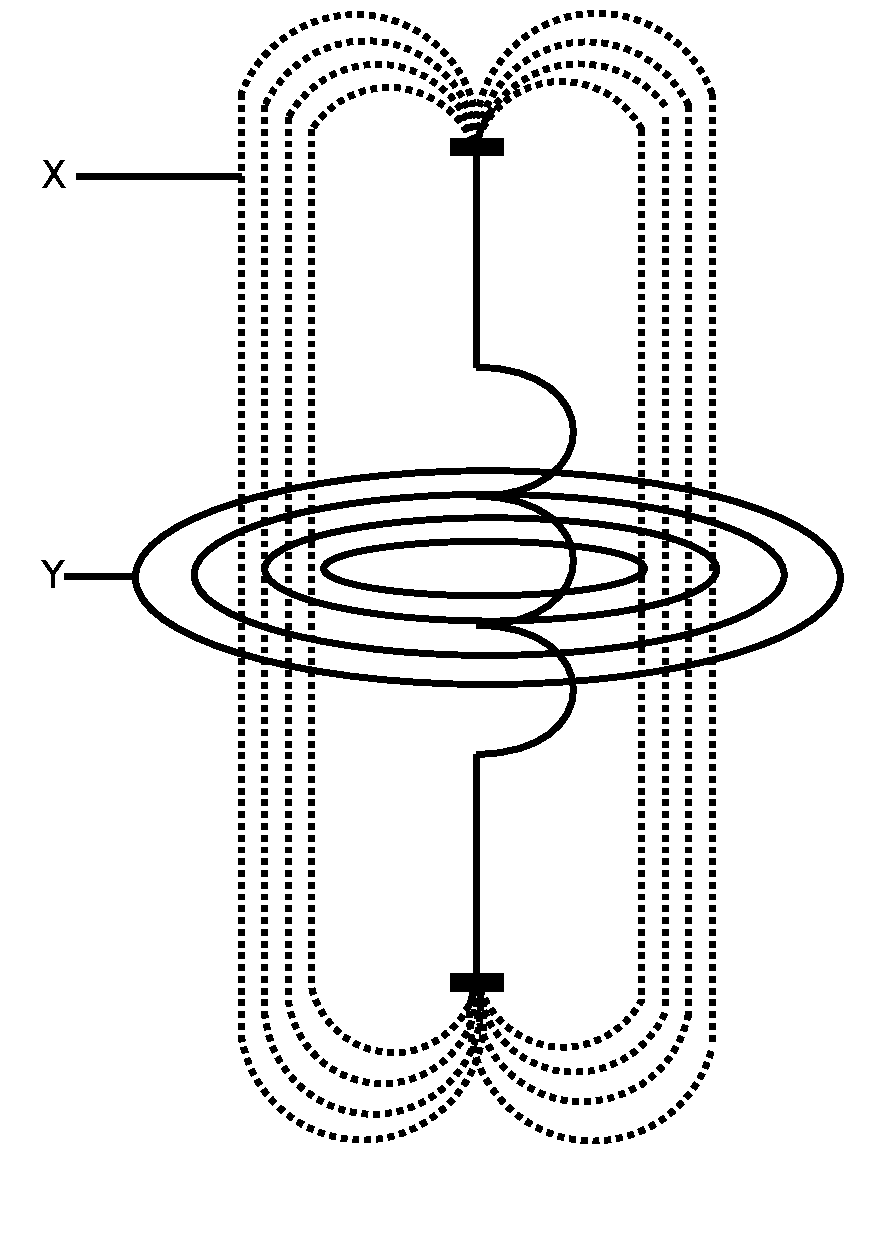
\includegraphics[scale=0.4]{Felder/Bilder/AntSchwingkreis_02.pdf}
% Graphic for TeX using PGF
% Title: /home/stole/Dokumente/git/afutub-kurs/Praxis/Skript/Felder/Bilder/AntSchwingkreis_02.dia
% Creator: Dia v0.97.3
% CreationDate: Sun Nov 22 15:48:43 2015
% For: stole
% \usepackage{tikz}
% The following commands are not supported in PSTricks at present
% We define them conditionally, so when they are implemented,
% this pgf file will use them.
\ifx\du\undefined
  \newlength{\du}
\fi
\setlength{\du}{15\unitlength}
\begin{tikzpicture}
\pgftransformxscale{1.000000}
\pgftransformyscale{-1.000000}
\definecolor{dialinecolor}{rgb}{0.000000, 0.000000, 0.000000}
\pgfsetstrokecolor{dialinecolor}
\definecolor{dialinecolor}{rgb}{1.000000, 1.000000, 1.000000}
\pgfsetfillcolor{dialinecolor}
\pgfsetlinewidth{0.100000\du}
\pgfsetdash{}{0pt}
\pgfsetdash{}{0pt}
\pgfsetbuttcap
\pgfsetmiterjoin
\pgfsetbuttcap
\pgfsetmiterjoin
\pgfsetdash{}{0pt}
\definecolor{dialinecolor}{rgb}{0.000000, 0.000000, 0.000000}
\pgfsetstrokecolor{dialinecolor}
\pgfpathmoveto{\pgfpoint{37.800000\du}{6.243424\du}}
\pgfpathcurveto{\pgfpoint{39.991233\du}{6.243424\du}}{\pgfpoint{39.991233\du}{8.434657\du}}{\pgfpoint{37.800000\du}{8.434657\du}}
\pgfusepath{stroke}
\pgfsetbuttcap
\pgfsetmiterjoin
\pgfsetdash{}{0pt}
\definecolor{dialinecolor}{rgb}{0.000000, 0.000000, 0.000000}
\pgfsetstrokecolor{dialinecolor}
\pgfpathmoveto{\pgfpoint{37.800000\du}{8.434657\du}}
\pgfpathcurveto{\pgfpoint{39.991233\du}{8.434657\du}}{\pgfpoint{39.991233\du}{10.625890\du}}{\pgfpoint{37.800000\du}{10.625890\du}}
\pgfusepath{stroke}
\pgfsetbuttcap
\pgfsetmiterjoin
\pgfsetdash{}{0pt}
\definecolor{dialinecolor}{rgb}{0.000000, 0.000000, 0.000000}
\pgfsetstrokecolor{dialinecolor}
\pgfpathmoveto{\pgfpoint{37.800000\du}{10.625890\du}}
\pgfpathcurveto{\pgfpoint{39.991233\du}{10.625890\du}}{\pgfpoint{39.991233\du}{12.817122\du}}{\pgfpoint{37.800000\du}{12.817122\du}}
\pgfusepath{stroke}
\pgfsetbuttcap
\pgfsetmiterjoin
\pgfsetdash{}{0pt}
\definecolor{dialinecolor}{rgb}{0.000000, 0.000000, 0.000000}
\pgfsetstrokecolor{dialinecolor}
\draw (37.800000\du,6.243424\du)--(37.800000\du,5.147808\du)--(37.800000\du,5.147808\du)--(37.800000\du,4.600000\du);
\pgfsetbuttcap
\pgfsetmiterjoin
\pgfsetdash{}{0pt}
\definecolor{dialinecolor}{rgb}{0.000000, 0.000000, 0.000000}
\pgfsetstrokecolor{dialinecolor}
\draw (37.800000\du,12.817122\du)--(37.800000\du,12.844513\du)--(37.800000\du,14.433156\du)--(37.800000\du,14.460547\du);
\pgfsetlinewidth{0.100000\du}
\pgfsetdash{}{0pt}
\pgfsetdash{}{0pt}
\definecolor{dialinecolor}{rgb}{0.000000, 0.000000, 0.000000}
\pgfsetstrokecolor{dialinecolor}
\pgfpathellipse{\pgfpoint{37.923500\du}{9.662689\du}}{\pgfpoint{2.723500\du}{0\du}}{\pgfpoint{0\du}{0.462689\du}}
\pgfusepath{stroke}
\pgfsetlinewidth{0.100000\du}
\pgfsetdash{}{0pt}
\pgfsetdash{}{0pt}
\definecolor{dialinecolor}{rgb}{0.000000, 0.000000, 0.000000}
\pgfsetstrokecolor{dialinecolor}
\pgfpathellipse{\pgfpoint{38.038619\du}{9.676882\du}}{\pgfpoint{3.838619\du}{0\du}}{\pgfpoint{0\du}{0.876882\du}}
\pgfusepath{stroke}
\pgfsetlinewidth{0.100000\du}
\pgfsetdash{}{0pt}
\pgfsetdash{}{0pt}
\definecolor{dialinecolor}{rgb}{0.000000, 0.000000, 0.000000}
\pgfsetstrokecolor{dialinecolor}
\pgfpathellipse{\pgfpoint{38.010905\du}{9.769417\du}}{\pgfpoint{5.010905\du}{0\du}}{\pgfpoint{0\du}{1.369417\du}}
\pgfusepath{stroke}
\pgfsetlinewidth{0.100000\du}
\pgfsetdash{}{0pt}
\pgfsetdash{}{0pt}
\definecolor{dialinecolor}{rgb}{0.000000, 0.000000, 0.000000}
\pgfsetstrokecolor{dialinecolor}
\pgfpathellipse{\pgfpoint{37.989095\du}{9.816259\du}}{\pgfpoint{5.989095\du}{0\du}}{\pgfpoint{0\du}{1.816259\du}}
\pgfusepath{stroke}
\pgfsetlinewidth{0.100000\du}
\pgfsetdash{}{0pt}
\pgfsetdash{}{0pt}
\pgfsetbuttcap
{
\definecolor{dialinecolor}{rgb}{0.000000, 0.000000, 0.000000}
\pgfsetfillcolor{dialinecolor}
% was here!!!
\definecolor{dialinecolor}{rgb}{0.000000, 0.000000, 0.000000}
\pgfsetstrokecolor{dialinecolor}
\draw (37.800000\du,4.600000\du)--(37.800000\du,2.600000\du);
}
\pgfsetlinewidth{0.100000\du}
\pgfsetdash{}{0pt}
\pgfsetdash{}{0pt}
\pgfsetbuttcap
{
\definecolor{dialinecolor}{rgb}{0.000000, 0.000000, 0.000000}
\pgfsetfillcolor{dialinecolor}
% was here!!!
\definecolor{dialinecolor}{rgb}{0.000000, 0.000000, 0.000000}
\pgfsetstrokecolor{dialinecolor}
\draw (37.800000\du,13.638835\du)--(37.800000\du,16.600000\du);
}
\pgfsetlinewidth{0.100000\du}
\pgfsetdash{{\pgflinewidth}{0.200000\du}}{0cm}
\pgfsetdash{{\pgflinewidth}{0.200000\du}}{0cm}
\pgfsetbuttcap
{
\definecolor{dialinecolor}{rgb}{0.000000, 0.000000, 0.000000}
\pgfsetfillcolor{dialinecolor}
% was here!!!
\definecolor{dialinecolor}{rgb}{0.000000, 0.000000, 0.000000}
\pgfsetstrokecolor{dialinecolor}
\draw (33.800000\du,1.600000\du)--(33.800000\du,17.800000\du);
}
\pgfsetlinewidth{0.100000\du}
\pgfsetdash{{\pgflinewidth}{0.200000\du}}{0cm}
\pgfsetdash{{\pgflinewidth}{0.200000\du}}{0cm}
\pgfsetbuttcap
{
\definecolor{dialinecolor}{rgb}{0.000000, 0.000000, 0.000000}
\pgfsetfillcolor{dialinecolor}
% was here!!!
\definecolor{dialinecolor}{rgb}{0.000000, 0.000000, 0.000000}
\pgfsetstrokecolor{dialinecolor}
\draw (34.200000\du,1.800000\du)--(34.200000\du,17.400000\du);
}
\pgfsetlinewidth{0.100000\du}
\pgfsetdash{{\pgflinewidth}{0.200000\du}}{0cm}
\pgfsetdash{{\pgflinewidth}{0.200000\du}}{0cm}
\pgfsetbuttcap
{
\definecolor{dialinecolor}{rgb}{0.000000, 0.000000, 0.000000}
\pgfsetfillcolor{dialinecolor}
% was here!!!
\definecolor{dialinecolor}{rgb}{0.000000, 0.000000, 0.000000}
\pgfsetstrokecolor{dialinecolor}
\draw (34.600000\du,2.000000\du)--(34.600000\du,17.000000\du);
}
\pgfsetlinewidth{0.100000\du}
\pgfsetdash{{\pgflinewidth}{0.200000\du}}{0cm}
\pgfsetdash{{\pgflinewidth}{0.200000\du}}{0cm}
\pgfsetbuttcap
{
\definecolor{dialinecolor}{rgb}{0.000000, 0.000000, 0.000000}
\pgfsetfillcolor{dialinecolor}
% was here!!!
\definecolor{dialinecolor}{rgb}{0.000000, 0.000000, 0.000000}
\pgfsetstrokecolor{dialinecolor}
\draw (35.000000\du,2.200000\du)--(35.000000\du,16.800000\du);
}
\pgfsetlinewidth{0.100000\du}
\pgfsetdash{{\pgflinewidth}{0.200000\du}}{0cm}
\pgfsetdash{{\pgflinewidth}{0.200000\du}}{0cm}
\pgfsetbuttcap
{
\definecolor{dialinecolor}{rgb}{0.000000, 0.000000, 0.000000}
\pgfsetfillcolor{dialinecolor}
% was here!!!
\definecolor{dialinecolor}{rgb}{0.000000, 0.000000, 0.000000}
\pgfsetstrokecolor{dialinecolor}
\pgfpathmoveto{\pgfpoint{37.799972\du}{2.600212\du}}
\pgfpatharc{8}{-159}{2.074477\du and 2.074477\du}
\pgfusepath{stroke}
}
\pgfsetlinewidth{0.100000\du}
\pgfsetdash{{\pgflinewidth}{0.200000\du}}{0cm}
\pgfsetdash{{\pgflinewidth}{0.200000\du}}{0cm}
\pgfsetbuttcap
{
\definecolor{dialinecolor}{rgb}{0.000000, 0.000000, 0.000000}
\pgfsetfillcolor{dialinecolor}
% was here!!!
\definecolor{dialinecolor}{rgb}{0.000000, 0.000000, 0.000000}
\pgfsetstrokecolor{dialinecolor}
\pgfpathmoveto{\pgfpoint{37.799998\du}{2.600198\du}}
\pgfpatharc{1}{-155}{1.884151\du and 1.884151\du}
\pgfusepath{stroke}
}
\pgfsetlinewidth{0.100000\du}
\pgfsetdash{{\pgflinewidth}{0.200000\du}}{0cm}
\pgfsetdash{{\pgflinewidth}{0.200000\du}}{0cm}
\pgfsetbuttcap
{
\definecolor{dialinecolor}{rgb}{0.000000, 0.000000, 0.000000}
\pgfsetfillcolor{dialinecolor}
% was here!!!
\definecolor{dialinecolor}{rgb}{0.000000, 0.000000, 0.000000}
\pgfsetstrokecolor{dialinecolor}
\pgfpathmoveto{\pgfpoint{37.800000\du}{2.600003\du}}
\pgfpatharc{354}{208}{1.705063\du and 1.705063\du}
\pgfusepath{stroke}
}
\pgfsetlinewidth{0.100000\du}
\pgfsetdash{{\pgflinewidth}{0.200000\du}}{0cm}
\pgfsetdash{{\pgflinewidth}{0.200000\du}}{0cm}
\pgfsetbuttcap
{
\definecolor{dialinecolor}{rgb}{0.000000, 0.000000, 0.000000}
\pgfsetfillcolor{dialinecolor}
% was here!!!
\definecolor{dialinecolor}{rgb}{0.000000, 0.000000, 0.000000}
\pgfsetstrokecolor{dialinecolor}
\pgfpathmoveto{\pgfpoint{37.800002\du}{2.600007\du}}
\pgfpatharc{344}{213}{1.557403\du and 1.557403\du}
\pgfusepath{stroke}
}
\pgfsetlinewidth{0.100000\du}
\pgfsetdash{{\pgflinewidth}{0.200000\du}}{0cm}
\pgfsetdash{{\pgflinewidth}{0.200000\du}}{0cm}
\pgfsetbuttcap
{
\definecolor{dialinecolor}{rgb}{0.000000, 0.000000, 0.000000}
\pgfsetfillcolor{dialinecolor}
% was here!!!
\definecolor{dialinecolor}{rgb}{0.000000, 0.000000, 0.000000}
\pgfsetstrokecolor{dialinecolor}
\pgfpathmoveto{\pgfpoint{34.999981\du}{16.799922\du}}
\pgfpatharc{167}{6}{1.422765\du and 1.422765\du}
\pgfusepath{stroke}
}
\pgfsetlinewidth{0.100000\du}
\pgfsetdash{{\pgflinewidth}{0.200000\du}}{0cm}
\pgfsetdash{{\pgflinewidth}{0.200000\du}}{0cm}
\pgfsetbuttcap
{
\definecolor{dialinecolor}{rgb}{0.000000, 0.000000, 0.000000}
\pgfsetfillcolor{dialinecolor}
% was here!!!
\definecolor{dialinecolor}{rgb}{0.000000, 0.000000, 0.000000}
\pgfsetstrokecolor{dialinecolor}
\pgfpathmoveto{\pgfpoint{34.599989\du}{16.999912\du}}
\pgfpatharc{173}{-7}{1.612452\du and 1.612452\du}
\pgfusepath{stroke}
}
\pgfsetlinewidth{0.100000\du}
\pgfsetdash{{\pgflinewidth}{0.200000\du}}{0cm}
\pgfsetdash{{\pgflinewidth}{0.200000\du}}{0cm}
\pgfsetbuttcap
{
\definecolor{dialinecolor}{rgb}{0.000000, 0.000000, 0.000000}
\pgfsetfillcolor{dialinecolor}
% was here!!!
\definecolor{dialinecolor}{rgb}{0.000000, 0.000000, 0.000000}
\pgfsetstrokecolor{dialinecolor}
\pgfpathmoveto{\pgfpoint{34.199995\du}{17.199902\du}}
\pgfpatharc{177}{-15}{1.836032\du and 1.836032\du}
\pgfusepath{stroke}
}
\pgfsetlinewidth{0.100000\du}
\pgfsetdash{{\pgflinewidth}{0.200000\du}}{0cm}
\pgfsetdash{{\pgflinewidth}{0.200000\du}}{0cm}
\pgfsetbuttcap
{
\definecolor{dialinecolor}{rgb}{0.000000, 0.000000, 0.000000}
\pgfsetfillcolor{dialinecolor}
% was here!!!
\definecolor{dialinecolor}{rgb}{0.000000, 0.000000, 0.000000}
\pgfsetstrokecolor{dialinecolor}
\pgfpathmoveto{\pgfpoint{33.799984\du}{17.599887\du}}
\pgfpatharc{172}{-19}{2.071984\du and 2.071984\du}
\pgfusepath{stroke}
}
\pgfsetlinewidth{0.100000\du}
\pgfsetdash{{\pgflinewidth}{0.200000\du}}{0cm}
\pgfsetdash{{\pgflinewidth}{0.200000\du}}{0cm}
\pgfsetbuttcap
{
\definecolor{dialinecolor}{rgb}{0.000000, 0.000000, 0.000000}
\pgfsetfillcolor{dialinecolor}
% was here!!!
\definecolor{dialinecolor}{rgb}{0.000000, 0.000000, 0.000000}
\pgfsetstrokecolor{dialinecolor}
\draw (40.600000\du,2.200000\du)--(40.600000\du,17.000000\du);
}
\pgfsetlinewidth{0.100000\du}
\pgfsetdash{{\pgflinewidth}{0.200000\du}}{0cm}
\pgfsetdash{{\pgflinewidth}{0.200000\du}}{0cm}
\pgfsetbuttcap
{
\definecolor{dialinecolor}{rgb}{0.000000, 0.000000, 0.000000}
\pgfsetfillcolor{dialinecolor}
% was here!!!
\definecolor{dialinecolor}{rgb}{0.000000, 0.000000, 0.000000}
\pgfsetstrokecolor{dialinecolor}
\draw (41.000000\du,2.000000\du)--(41.000000\du,17.200000\du);
}
\pgfsetlinewidth{0.100000\du}
\pgfsetdash{{\pgflinewidth}{0.200000\du}}{0cm}
\pgfsetdash{{\pgflinewidth}{0.200000\du}}{0cm}
\pgfsetbuttcap
{
\definecolor{dialinecolor}{rgb}{0.000000, 0.000000, 0.000000}
\pgfsetfillcolor{dialinecolor}
% was here!!!
\definecolor{dialinecolor}{rgb}{0.000000, 0.000000, 0.000000}
\pgfsetstrokecolor{dialinecolor}
\draw (41.400000\du,1.800000\du)--(41.400000\du,17.400000\du);
}
\pgfsetlinewidth{0.100000\du}
\pgfsetdash{{\pgflinewidth}{0.200000\du}}{0cm}
\pgfsetdash{{\pgflinewidth}{0.200000\du}}{0cm}
\pgfsetbuttcap
{
\definecolor{dialinecolor}{rgb}{0.000000, 0.000000, 0.000000}
\pgfsetfillcolor{dialinecolor}
% was here!!!
\definecolor{dialinecolor}{rgb}{0.000000, 0.000000, 0.000000}
\pgfsetstrokecolor{dialinecolor}
\draw (41.800000\du,1.600000\du)--(41.800000\du,17.800000\du);
}
\pgfsetlinewidth{0.100000\du}
\pgfsetdash{{\pgflinewidth}{0.200000\du}}{0cm}
\pgfsetdash{{\pgflinewidth}{0.200000\du}}{0cm}
\pgfsetbuttcap
{
\definecolor{dialinecolor}{rgb}{0.000000, 0.000000, 0.000000}
\pgfsetfillcolor{dialinecolor}
% was here!!!
\definecolor{dialinecolor}{rgb}{0.000000, 0.000000, 0.000000}
\pgfsetstrokecolor{dialinecolor}
\pgfpathmoveto{\pgfpoint{41.800004\du}{1.600011\du}}
\pgfpatharc{341}{172}{2.071632\du and 2.071632\du}
\pgfusepath{stroke}
}
\pgfsetlinewidth{0.100000\du}
\pgfsetdash{{\pgflinewidth}{0.200000\du}}{0cm}
\pgfsetdash{{\pgflinewidth}{0.200000\du}}{0cm}
\pgfsetbuttcap
{
\definecolor{dialinecolor}{rgb}{0.000000, 0.000000, 0.000000}
\pgfsetfillcolor{dialinecolor}
% was here!!!
\definecolor{dialinecolor}{rgb}{0.000000, 0.000000, 0.000000}
\pgfsetstrokecolor{dialinecolor}
\pgfpathmoveto{\pgfpoint{41.400006\du}{1.800013\du}}
\pgfpatharc{335}{187}{1.896166\du and 1.896166\du}
\pgfusepath{stroke}
}
\pgfsetlinewidth{0.100000\du}
\pgfsetdash{{\pgflinewidth}{0.200000\du}}{0cm}
\pgfsetdash{{\pgflinewidth}{0.200000\du}}{0cm}
\pgfsetbuttcap
{
\definecolor{dialinecolor}{rgb}{0.000000, 0.000000, 0.000000}
\pgfsetfillcolor{dialinecolor}
% was here!!!
\definecolor{dialinecolor}{rgb}{0.000000, 0.000000, 0.000000}
\pgfsetstrokecolor{dialinecolor}
\pgfpathmoveto{\pgfpoint{41.000012\du}{1.800016\du}}
\pgfpatharc{323}{197}{1.825000\du and 1.825000\du}
\pgfusepath{stroke}
}
\pgfsetlinewidth{0.100000\du}
\pgfsetdash{{\pgflinewidth}{0.200000\du}}{0cm}
\pgfsetdash{{\pgflinewidth}{0.200000\du}}{0cm}
\pgfsetbuttcap
{
\definecolor{dialinecolor}{rgb}{0.000000, 0.000000, 0.000000}
\pgfsetfillcolor{dialinecolor}
% was here!!!
\definecolor{dialinecolor}{rgb}{0.000000, 0.000000, 0.000000}
\pgfsetstrokecolor{dialinecolor}
\pgfpathmoveto{\pgfpoint{40.600006\du}{2.200011\du}}
\pgfpatharc{332}{200}{1.536070\du and 1.536070\du}
\pgfusepath{stroke}
}
\pgfsetlinewidth{0.100000\du}
\pgfsetdash{{\pgflinewidth}{0.200000\du}}{0cm}
\pgfsetdash{{\pgflinewidth}{0.200000\du}}{0cm}
\pgfsetbuttcap
{
\definecolor{dialinecolor}{rgb}{0.000000, 0.000000, 0.000000}
\pgfsetfillcolor{dialinecolor}
% was here!!!
\definecolor{dialinecolor}{rgb}{0.000000, 0.000000, 0.000000}
\pgfsetstrokecolor{dialinecolor}
\pgfpathmoveto{\pgfpoint{37.799983\du}{16.599917\du}}
\pgfpatharc{169}{29}{1.505127\du and 1.505127\du}
\pgfusepath{stroke}
}
\pgfsetlinewidth{0.100000\du}
\pgfsetdash{{\pgflinewidth}{0.200000\du}}{0cm}
\pgfsetdash{{\pgflinewidth}{0.200000\du}}{0cm}
\pgfsetbuttcap
{
\definecolor{dialinecolor}{rgb}{0.000000, 0.000000, 0.000000}
\pgfsetfillcolor{dialinecolor}
% was here!!!
\definecolor{dialinecolor}{rgb}{0.000000, 0.000000, 0.000000}
\pgfsetstrokecolor{dialinecolor}
\pgfpathmoveto{\pgfpoint{37.800033\du}{16.599907\du}}
\pgfpatharc{200}{14}{2.090592\du and 2.090592\du}
\pgfusepath{stroke}
}
\pgfsetlinewidth{0.100000\du}
\pgfsetdash{{\pgflinewidth}{0.200000\du}}{0cm}
\pgfsetdash{{\pgflinewidth}{0.200000\du}}{0cm}
\pgfsetbuttcap
{
\definecolor{dialinecolor}{rgb}{0.000000, 0.000000, 0.000000}
\pgfsetfillcolor{dialinecolor}
% was here!!!
\definecolor{dialinecolor}{rgb}{0.000000, 0.000000, 0.000000}
\pgfsetstrokecolor{dialinecolor}
\pgfpathmoveto{\pgfpoint{37.800015\du}{16.599910\du}}
\pgfpatharc{190}{10}{1.824829\du and 1.824829\du}
\pgfusepath{stroke}
}
\pgfsetlinewidth{0.100000\du}
\pgfsetdash{{\pgflinewidth}{0.200000\du}}{0cm}
\pgfsetdash{{\pgflinewidth}{0.200000\du}}{0cm}
\pgfsetbuttcap
{
\definecolor{dialinecolor}{rgb}{0.000000, 0.000000, 0.000000}
\pgfsetfillcolor{dialinecolor}
% was here!!!
\definecolor{dialinecolor}{rgb}{0.000000, 0.000000, 0.000000}
\pgfsetstrokecolor{dialinecolor}
\pgfpathmoveto{\pgfpoint{37.799998\du}{16.599912\du}}
\pgfpatharc{179}{23}{1.665213\du and 1.665213\du}
\pgfusepath{stroke}
}
\pgfsetlinewidth{0.100000\du}
\pgfsetdash{}{0pt}
\pgfsetdash{}{0pt}
\pgfsetmiterjoin
\definecolor{dialinecolor}{rgb}{0.000000, 0.000000, 0.000000}
\pgfsetfillcolor{dialinecolor}
\fill (37.400000\du,2.400000\du)--(37.400000\du,2.600000\du)--(38.200000\du,2.600000\du)--(38.200000\du,2.400000\du)--cycle;
\definecolor{dialinecolor}{rgb}{0.000000, 0.000000, 0.000000}
\pgfsetstrokecolor{dialinecolor}
\draw (37.400000\du,2.400000\du)--(37.400000\du,2.600000\du)--(38.200000\du,2.600000\du)--(38.200000\du,2.400000\du)--cycle;
\pgfsetlinewidth{0.100000\du}
\pgfsetdash{}{0pt}
\pgfsetdash{}{0pt}
\pgfsetmiterjoin
\definecolor{dialinecolor}{rgb}{0.000000, 0.000000, 0.000000}
\pgfsetfillcolor{dialinecolor}
\fill (37.400000\du,16.600000\du)--(37.400000\du,16.800000\du)--(38.200000\du,16.800000\du)--(38.200000\du,16.600000\du)--cycle;
\definecolor{dialinecolor}{rgb}{0.000000, 0.000000, 0.000000}
\pgfsetstrokecolor{dialinecolor}
\draw (37.400000\du,16.600000\du)--(37.400000\du,16.800000\du)--(38.200000\du,16.800000\du)--(38.200000\du,16.600000\du)--cycle;
% setfont left to latex
\definecolor{dialinecolor}{rgb}{0.000000, 0.000000, 0.000000}
\pgfsetstrokecolor{dialinecolor}
\node[anchor=west] at (30.106062\du,1.530310\du){X};
% setfont left to latex
\definecolor{dialinecolor}{rgb}{0.000000, 0.000000, 0.000000}
\pgfsetstrokecolor{dialinecolor}
\node[anchor=west] at (30.132142\du,9.530298\du){Y};
\pgfsetlinewidth{0.100000\du}
\pgfsetdash{}{0pt}
\pgfsetdash{}{0pt}
\pgfsetbuttcap
{
\definecolor{dialinecolor}{rgb}{0.000000, 0.000000, 0.000000}
\pgfsetfillcolor{dialinecolor}
% was here!!!
\definecolor{dialinecolor}{rgb}{0.000000, 0.000000, 0.000000}
\pgfsetstrokecolor{dialinecolor}
\draw (31.000000\du,1.800000\du)--(33.800000\du,1.800000\du);
}
\pgfsetlinewidth{0.100000\du}
\pgfsetdash{}{0pt}
\pgfsetdash{}{0pt}
\pgfsetbuttcap
{
\definecolor{dialinecolor}{rgb}{0.000000, 0.000000, 0.000000}
\pgfsetfillcolor{dialinecolor}
% was here!!!
\definecolor{dialinecolor}{rgb}{0.000000, 0.000000, 0.000000}
\pgfsetstrokecolor{dialinecolor}
\draw (31.000000\du,9.800000\du)--(31.980000\du,9.800000\du);
}
\end{tikzpicture}

\caption{Elektromagnetisches Feld bei der Vertikalantenne}
\label{AntSchwingkreis_02}
\end{figure}

\begin{enumerate} 
\itemsep1pt\parskip0pt\parsep0pt
\item[6] \emph{\textbf{TB303}} Wie werden die mit X gekennzeichneten Feldlinien einer Vertikalantenne bezeichnet (siehe Abbildung \ref{AntSchwingkreis_02})?
	\begin{enumerate}
	\itemsep1pt\parskip0pt\parsep0pt
		\item[A] Magnetische Feldlinien
		\item[B] Elektrische Feldlinien
		\item[C] Polarisierte Feldlinien
		\item[D] Horizontale Feldlinien
		\loesung{Lösung B}
	\end{enumerate}
\end{enumerate}


\begin{enumerate} 
\itemsep1pt\parskip0pt\parsep0pt
\item[7] \emph{\textbf{TB404}} Wie werden die mit Y gekennzeichneten Feldlinien einer Vertikalantenne bezeichnet (siehe Abbildung \ref{AntSchwingkreis_02})?
	\begin{enumerate}
	\itemsep1pt\parskip0pt\parsep0pt
		\item[A] Magnetische Feldlinien
		\item[B] Elektrische Feldlinien
		\item[C] Radiale Feldlinien
		\item[D] Vertikale Feldlinien
		\loesung{Lösung A}
	\end{enumerate}
\end{enumerate}

\begin{enumerate} 
\itemsep1pt\parskip0pt\parsep0pt
\item[8] \emph{\textbf{TB602}} Welcher Wellenlänge $\lambda$ entspricht die Frequenz $1,84 MHz$?
	\begin{enumerate}
	\itemsep1pt\parskip0pt\parsep0pt
		\item[A] $16,3m$
		\item[B] $163m$
		\item[C] $0,163m$
		\item[D] $16,3m$
		\loesung{Lösung B; $\lambda = \dfrac{c}{f}$}
	\end{enumerate}
\end{enumerate}

\mucho{9}{TB501}
{ Wodurch entsteht ein elektromagnetisches Feld? 
Ein elektromagnetisches Feld entsteht,}%Frage
{wenn ein zeitlich schnell veränderlicher Strom durch einen elektrischen Leiter fließt, dessen Länge mindestens 1/100 der Wellenlänge ist.}%A
{	wenn durch einen elektrischen Leiter, dessen Länge mindestens 1/100 der Wellenlänge ist, ein konstanter Strom fließt.}%B
{wenn sich elektrische Ladungen in einem Leiter befinden, dessen Länge mindestens 1/100 der Wellenlänge ist.}%C
{	wenn an einem elektrischen Leiter, dessen Länge mindestens 1/100 der Wellenlänge ist, eine konstante Spannung angelegt wird.}%D
{A}%Lösung

\newpage \vspace*{5cm}
\newpage

\chapter{Die Wellenausbreitung}
\begin{wrapfigure}[0]{r}[-1cm]{4cm}
 \vspace{-6cm}
  \includegraphics[scale=0.04]{Wellenausbreitung/Bilder/aurora.jpeg}
 \vspace{-6cm}
\end{wrapfigure}

\section*{Theorie- und Prüfungsfragen}


\subsection*{Kurzwellenausbreitung}

\begin{enumerate} 
\itemsep1pt\parskip0pt\parsep0pt
\item[1] \emph{\textbf{TI203}}  Welche der folgenden Aussagen trifft für KW-Funkverbindungen zu, die über Bodenwellen erfolgen? Die Bodenwelle folgt der Erdkrümmung und ...
	\begin{enumerate}
	\itemsep1pt\parskip0pt\parsep0pt
		\item[A] geht nicht über den geografischen Horizont hinaus. Sie wird in höheren Frequenzbereichen stärker gedämpft als in niedrigeren Frequenzbereichen.
		\item[B] geht über den geografischen Horizont hinaus. Sie wird in niedrigeren Frequenzbereichen stärker gedämpft als in höheren Frequenzbereichen.
		\item[C] geht über den geografischen Horizont hinaus. Sie wird in höheren Frequenzbereichen stärker gedämpft als in niedrigeren Frequenzbereichen.
		\item[D] geht nicht über den geografischen Horizont hinaus. Sie wird in niedrigeren Frequenzbereichen stärker gedämpft als in höheren Frequenzbereichen.
		\loesung{Lösung C}
	\end{enumerate}
\end{enumerate}

\subsection*{Ionosphäre}

\begin{enumerate} 
\itemsep1pt\parskip0pt\parsep0pt
\item[2] \emph{\textbf{TI103}}  In welcher Höhe befinden sich die für die Fernausbreitung (DX) wichtigen ionosphärischen Schichten? Sie befinden sich in ungefähr ...
	\begin{enumerate}
	\itemsep1pt\parskip0pt\parsep0pt
		\item[A] 2 bis 5 km Höhe.
		\item[B] 20 bis 50 km Höhe.
		\item[C] 200 bis 500 km Höhe.
		\item[D] 2000 bis 5000 km Höhe.
		\loesung{Lösung C}
	\end{enumerate}
\end{enumerate}

\begin{enumerate} 
\itemsep1pt\parskip0pt\parsep0pt
\item[3] Ergänze folgendes Schaubild: Abbildung  \ref{welle}. Tragen Sie die Bezeichnungen der einzelnen Schichten ein, die Höhe in der sie sich etwa befindet und die wichtigsten Frequenzen.
\end{enumerate}

\begin{figure}[H]
\def\svgwidth{\columnwidth}
\input{Wellenausbreitung/Bilder/Wellenausbreitung2.pdf_tex}
\caption{Aufbau der Ionosphäre und reflektierende Eigenschaften der Schichten}
\label{welle}
\end{figure}

% FIXME Hier muss markiert werden welche für die Prüfung wirklich wichtig sind!

\loesung{
\begin{figure}[H]
\def\svgwidth{\columnwidth}
\begin{wrapfigure}[0]{r}[-1cm]{4cm}
 \vspace{-6cm}
  \includegraphics[scale=0.04]{Wellenausbreitung/Bilder/aurora.jpeg}
 \vspace{-6cm}
\end{wrapfigure}

\section*{Theorie- und Prüfungsfragen}


\subsection*{Kurzwellenausbreitung}

\begin{enumerate} 
\itemsep1pt\parskip0pt\parsep0pt
\item[1] \emph{\textbf{TI203}}  Welche der folgenden Aussagen trifft für KW-Funkverbindungen zu, die über Bodenwellen erfolgen? Die Bodenwelle folgt der Erdkrümmung und ...
	\begin{enumerate}
	\itemsep1pt\parskip0pt\parsep0pt
		\item[A] geht nicht über den geografischen Horizont hinaus. Sie wird in höheren Frequenzbereichen stärker gedämpft als in niedrigeren Frequenzbereichen.
		\item[B] geht über den geografischen Horizont hinaus. Sie wird in niedrigeren Frequenzbereichen stärker gedämpft als in höheren Frequenzbereichen.
		\item[C] geht über den geografischen Horizont hinaus. Sie wird in höheren Frequenzbereichen stärker gedämpft als in niedrigeren Frequenzbereichen.
		\item[D] geht nicht über den geografischen Horizont hinaus. Sie wird in niedrigeren Frequenzbereichen stärker gedämpft als in höheren Frequenzbereichen.
		\loesung{Lösung C}
	\end{enumerate}
\end{enumerate}

\subsection*{Ionosphäre}

\begin{enumerate} 
\itemsep1pt\parskip0pt\parsep0pt
\item[2] \emph{\textbf{TI103}}  In welcher Höhe befinden sich die für die Fernausbreitung (DX) wichtigen ionosphärischen Schichten? Sie befinden sich in ungefähr ...
	\begin{enumerate}
	\itemsep1pt\parskip0pt\parsep0pt
		\item[A] 2 bis 5 km Höhe.
		\item[B] 20 bis 50 km Höhe.
		\item[C] 200 bis 500 km Höhe.
		\item[D] 2000 bis 5000 km Höhe.
		\loesung{Lösung C}
	\end{enumerate}
\end{enumerate}

\begin{enumerate} 
\itemsep1pt\parskip0pt\parsep0pt
\item[3] Ergänze folgendes Schaubild: Abbildung  \ref{welle}. Tragen Sie die Bezeichnungen der einzelnen Schichten ein, die Höhe in der sie sich etwa befindet und die wichtigsten Frequenzen.
\end{enumerate}

\begin{figure}[H]
\def\svgwidth{\columnwidth}
\input{Wellenausbreitung/Bilder/Wellenausbreitung2.pdf_tex}
\caption{Aufbau der Ionosphäre und reflektierende Eigenschaften der Schichten}
\label{welle}
\end{figure}

% FIXME Hier muss markiert werden welche für die Prüfung wirklich wichtig sind!

\loesung{
\begin{figure}[H]
\def\svgwidth{\columnwidth}
\begin{wrapfigure}[0]{r}[-1cm]{4cm}
 \vspace{-6cm}
  \includegraphics[scale=0.04]{Wellenausbreitung/Bilder/aurora.jpeg}
 \vspace{-6cm}
\end{wrapfigure}

\section*{Theorie- und Prüfungsfragen}


\subsection*{Kurzwellenausbreitung}

\begin{enumerate} 
\itemsep1pt\parskip0pt\parsep0pt
\item[1] \emph{\textbf{TI203}}  Welche der folgenden Aussagen trifft für KW-Funkverbindungen zu, die über Bodenwellen erfolgen? Die Bodenwelle folgt der Erdkrümmung und ...
	\begin{enumerate}
	\itemsep1pt\parskip0pt\parsep0pt
		\item[A] geht nicht über den geografischen Horizont hinaus. Sie wird in höheren Frequenzbereichen stärker gedämpft als in niedrigeren Frequenzbereichen.
		\item[B] geht über den geografischen Horizont hinaus. Sie wird in niedrigeren Frequenzbereichen stärker gedämpft als in höheren Frequenzbereichen.
		\item[C] geht über den geografischen Horizont hinaus. Sie wird in höheren Frequenzbereichen stärker gedämpft als in niedrigeren Frequenzbereichen.
		\item[D] geht nicht über den geografischen Horizont hinaus. Sie wird in niedrigeren Frequenzbereichen stärker gedämpft als in höheren Frequenzbereichen.
		\loesung{Lösung C}
	\end{enumerate}
\end{enumerate}

\subsection*{Ionosphäre}

\begin{enumerate} 
\itemsep1pt\parskip0pt\parsep0pt
\item[2] \emph{\textbf{TI103}}  In welcher Höhe befinden sich die für die Fernausbreitung (DX) wichtigen ionosphärischen Schichten? Sie befinden sich in ungefähr ...
	\begin{enumerate}
	\itemsep1pt\parskip0pt\parsep0pt
		\item[A] 2 bis 5 km Höhe.
		\item[B] 20 bis 50 km Höhe.
		\item[C] 200 bis 500 km Höhe.
		\item[D] 2000 bis 5000 km Höhe.
		\loesung{Lösung C}
	\end{enumerate}
\end{enumerate}

\begin{enumerate} 
\itemsep1pt\parskip0pt\parsep0pt
\item[3] Ergänze folgendes Schaubild: Abbildung  \ref{welle}. Tragen Sie die Bezeichnungen der einzelnen Schichten ein, die Höhe in der sie sich etwa befindet und die wichtigsten Frequenzen.
\end{enumerate}

\begin{figure}[H]
\def\svgwidth{\columnwidth}
\input{Wellenausbreitung/Bilder/Wellenausbreitung2.pdf_tex}
\caption{Aufbau der Ionosphäre und reflektierende Eigenschaften der Schichten}
\label{welle}
\end{figure}

% FIXME Hier muss markiert werden welche für die Prüfung wirklich wichtig sind!

\loesung{
\begin{figure}[H]
\def\svgwidth{\columnwidth}
\input{Wellenausbreitung/Bilder/Wellenausbreitung.pdf_tex}
\end{figure}
}

\subsection*{Sonnenflecken}

\begin{enumerate} 
\itemsep1pt\parskip0pt\parsep0pt
\item[4] \emph{\textbf{TI107}}  Die Sonnenfleckenzahl ist einem regelmäßigen Zyklus unterworfen. Welchen Zeitraum hat dieser Zyklus zirka?
	\begin{enumerate}
	\itemsep1pt\parskip0pt\parsep0pt
		\item[A] 6 Monate
		\item[B] 12 Monate
		\item[C] 100 Jahre
		\item[D] 11 Jahre
	\loesung{Lösung D}
	\end{enumerate}
\end{enumerate}


\subsection*{Reichweite der Raumwellen}

\begin{enumerate} 
\itemsep1pt\parskip0pt\parsep0pt
\item[5] Was bedeutet die Abkürzung $MUF$? \loesung{Von Ionosphärenmessstationen wird die so genannte kritische Frequenz $f_k$ gemessen. Das ist die höchste Frequenz, bei der die senkrecht in die Ionosphäre eintretende Raumwelle gerade noch reflektiert wird. Daraus ergibt sich die obere brauchbare Grenzfrequenz $MUF$ (maximum usable frequency) durch das so genannte Sekansgesetz:}
\item[6] \emph{\textbf{TI212}}   Was bedeutet die $MUF$ bei der Kurzwellenausbreitung?
	\begin{enumerate}
	\itemsep1pt\parskip0pt\parsep0pt
		\item[A] Mittlere Nutzfrequenz
		\item[B] Höchste brauchbare Frequenz
		\item[C] Niedrigste brauchbare Frequenz
		\item[D] Kritische Grenzfrequenz
		\loesung{Lösung B}
	\end{enumerate}
\end{enumerate}

\begin{enumerate} 
\itemsep1pt\parskip0pt\parsep0pt
\item[7] \emph{\textbf{TI205}}   Von welchem der genannten Parameter ist die Sprungdistanz abhängig, die ein KW-Signal auf der Erdoberfläche überbrücken kann?
	\begin{enumerate}
	\itemsep1pt\parskip0pt\parsep0pt
		\item[A] Von der Polarisation der Antenne
		\item[B] Von der Sendeleistung
		\item[C] Vom Antennengewinn
		\item[D] Vom Abstrahlwinkel der Antenne
		\loesung{Lösung D}
	\end{enumerate}
\end{enumerate}

\subsection*{D-Schicht}

\begin{enumerate} 
\itemsep1pt\parskip0pt\parsep0pt
\item[8] \emph{\textbf{TI210}}   Warum sind Signale im 160- und 80-Meter-Band tagsüber nur schwach und nicht für den weltweiten Funkverkehr geeignet? Sie sind ungeeignet wegen der Tagesdämpfung in der ...
	\begin{enumerate}
	\itemsep1pt\parskip0pt\parsep0pt
		\item[A] A-Schicht
		\item[B] D-Schicht
		\item[C] F1-Schicht
		\item[D] F2-Schicht
		\loesung{Lösung B}
	\end{enumerate}
\end{enumerate}


\subsection*{Fading}

\begin{enumerate} 
\itemsep1pt\parskip0pt\parsep0pt
\item[9] Erläutere den Begriff Fading.
\loesung{Ionosphärischer Feldstärkeschwund durch Überlagerung von Boden- und Raumwelle, der sich bei der Kurzwellenausbreitung besonders bei AM-Sendungen bemerkbar macht}
\end{enumerate}

\subsection*{F- und E-Schicht}

\begin{enumerate} 
\itemsep1pt\parskip0pt\parsep0pt
\item[10] \emph{\textbf{TI106}}   Welche Schicht ist für die gute Ausbreitung im 10-m-Band in den Sommermonaten verantwortlich?
	\begin{enumerate}
	\itemsep1pt\parskip0pt\parsep0pt
		\item[A] D-Schicht
		\item[B] F1-Schicht
		\item[C] F2-Schicht
		\item[D] E-Schicht
		\loesung{Lösung D}
	\end{enumerate}
\end{enumerate}


\subsection*{Tote Zone}

\begin{enumerate} 
\itemsep1pt\parskip0pt\parsep0pt
\item[11] \emph{\textbf{TI202}}   Unter der ``Toten Zone'' wird der Bereich verstanden,
	\begin{enumerate}
	\itemsep1pt\parskip0pt\parsep0pt
		\item[A] der durch die Bodenwelle überdeckt wird, so dass schwächere DX-Stationen zugedeckt werden.
		\item[B] der durch die Bodenwelle erreicht wird und für die Raumwelle nicht zugänglich ist.
		\item[C] der durch die Bodenwelle nicht mehr erreicht wird und durch die reflektierte Raumwelle noch nicht erreicht wird.
		\item[D] der durch die Interferenz der Bodenwelle mit der Raumwelle in einer Zone der gegenseitigen Auslöschung liegt.
		\loesung{Lösung C}
	\end{enumerate}
\end{enumerate}

\subsection*{Kurzwelle}

\begin{enumerate} 
\itemsep1pt\parskip0pt\parsep0pt
\item[12] \emph{\textbf{TI206}}   Bei der Ausbreitung auf Kurzwelle spielt die so genannte ``Grey Line'' eine besondere Rolle. Was ist die ``Grey Line''?
	\begin{enumerate}
	\itemsep1pt\parskip0pt\parsep0pt
		\item[A] Die instabilen Ausbreitungsbedingungen in der Äquatorialzone.
		\item[B] Die Zeit mit den besten Möglichkeiten für ``Short Skip'' Ausbreitung.
		\item[C] Die Übergangszeit vor und nach dem Winter, in der sich die D-Schicht ab- und wieder aufbaut.
		\item[D] Der Streifen der Dämmerungsphase vor Sonnenaufgang oder nach Sonnenuntergang.
		\loesung{Lösung D}
	\end{enumerate}
\end{enumerate}

\begin{enumerate} 
\itemsep1pt\parskip0pt\parsep0pt
\item[13] Ergänze in der Tabelle die jeweiligen Frequenzbereiche für die einzelnen Bänder.
\end{enumerate}


\begin{figure}[H]
	\subfigure{
		\begin{tabular}{|r|l|}
			\hline
			Band 	& Frequenzbereich\\
			\hline
			$160m$ & ~\hspace*{4cm}\\
			$80m$  & ~\hspace*{4cm}\\
			$40m$  & ~\hspace*{4cm}\\
			$20m$  & ~\hspace*{4cm}\\
			$15m$  & ~\hspace*{4cm}\\
			$10m$  & ~\hspace*{4cm}\\
			\hline
		\end{tabular}
	}
	\subfigure{
		\loesung{
			\begin{tabular}{|r|l|}
				\hline
				Band 	& Frequenzbereich\\
				\hline
				$160m$ & $1,810-2,000MHz$\\
				$80m$  & $3,500-3,800MHz$\\
				$40m$  & $7,000-7,200MHz$\\
				$20m$  & $14,000-14,350MHz$\\
				$15m$  & $21,000-21,450MHz$\\
				$10m$  & $28,000-29,700MHz$\\
				\hline
			\end{tabular}
			}
	}
\end{figure}


\begin{enumerate} 
\itemsep1pt\parskip0pt\parsep0pt
\item[15] \emph{\textbf{TI210}}   Warum sind Signale im 160- und 80-Meter-Band tagsüber nur schwach und nicht für den weltweiten Funkverkehr geeignet? Sie sind ungeeignet wegen der Tagesdämpfung in der
	\begin{enumerate}
	\itemsep1pt\parskip0pt\parsep0pt
		\item[A] A-Schicht
		\item[B] D-Schicht
		\item[C] F1-Schicht
		\item[D] F2-Schicht
		\loesung{Lösung B}
	\end{enumerate}
\end{enumerate}

\subsection*{UKW}

\begin{enumerate} 
\itemsep1pt\parskip0pt\parsep0pt
\item[14] \emph{\textbf{TI301}}   Wie weit etwa reicht der Funkhorizont im UKW-Bereich über den geografischen Horizont hinaus? Er reicht etwa ...
	\begin{enumerate}
	\itemsep1pt\parskip0pt\parsep0pt
		\item[A] doppelt so weit.
		\item[B] bis zur Hälfte der Entfernung bis zum geografischen Horizont.
		\item[C] bis zum Vierfachen der Entfernung bis zum geografischen Horizont.
		\item[D] $15 \%$ weiter als der geografische Horizont.
		\loesung{Lösung D}
	\end{enumerate}
\end{enumerate}

\begin{enumerate} 
\itemsep1pt\parskip0pt\parsep0pt
\item[15] \emph{\textbf{TI305}}   Wie wirkt die Antennenhöhe auf die Reichweite einer UKW-Verbindung aus? Die Reichweite steigt mit zunehmender Antennenhöhe, weil ...
	\begin{enumerate}
	\itemsep1pt\parskip0pt\parsep0pt
		\item[A] die dämpfende Wirkung der Erdoberfläche abnimmt.
		\item[B] die Entfernung zu den reflektierenden Schichten der Troposphäre abnimmt.
		\item[C] in höheren Luftschichten die Temperatur sinkt.
		\item[D] die optische Sichtweite zunimmt.
		\loesung{Lösung D}
	\end{enumerate}
\end{enumerate}

\subsection*{Sporadic-E}

\begin{enumerate} 
\itemsep1pt\parskip0pt\parsep0pt
\item[16] \emph{\textbf{TI309}}   Was versteht man unter dem Begriff Sporadic E? Man versteht darunter ...
	\begin{enumerate}
	\itemsep1pt\parskip0pt\parsep0pt
		\item[A] kurzfristige plötzliche Inversionsänderungen in der E-Schicht, die Fernausbreitung im VHF-Bereich ermöglichen.
		\item[B] kurzzeitig auftretende starke Reflexion von VHF-Signalen an Meteorbahnen innerhalb der E-Schicht.
		\item[C] lokal begrenzten kurzzeitigen Ausfall der Reflexion durch ungewöhnlich hohe Ionisation innerhalb der E-Schicht.
		\item[D] die Reflexion an lokal begrenzten Bereichen mit ungewöhnlich hoher Ionisation innerhalb der E-Schicht.
		\loesung{Lösung D}
	\end{enumerate}
\end{enumerate}

\begin{enumerate} 
\itemsep1pt\parskip0pt\parsep0pt
\item[17] \emph{\textbf{TI204}}  Wie groß ist in etwa die maximale Entfernung, die ein KW-Signal bei Reflexion an der E-Schicht auf der Erdoberfläche mit einem Sprung (Hop) überbrücken kann?
	\begin{enumerate}
	\itemsep1pt\parskip0pt\parsep0pt
		\item[A] Etwa 1100 km
		\item[B] Etwa 2200 km
		\item[C] Etwa 4500 km
		\item[D] Etwa 9000 km
		\loesung{Lösung B}
	\end{enumerate}
\end{enumerate}

\subsection*{Aurora}

\begin{enumerate} 
\itemsep1pt\parskip0pt\parsep0pt
\item[18] \emph{\textbf{TI211}}   In welcher ionosphärischen Schicht treten gelegentlich Aurora-Erscheinungen auf?
	\begin{enumerate}
	\itemsep1pt\parskip0pt\parsep0pt
		\item[A] In der F-Schicht
		\item[B] In der E-Schicht Nähe des Äquators
		\item[C] In der E-Schicht
		\item[D] In der D-Schicht
		\loesung{Lösung C}
	\end{enumerate}
\end{enumerate}

\begin{enumerate} 
\itemsep1pt\parskip0pt\parsep0pt
\item[19] \emph{\textbf{TI306}} Was ist die Ursache für Aurora-Erscheinungen? Die Ursache ist ...
	\begin{enumerate}
	\itemsep1pt\parskip0pt\parsep0pt
		\item[A] das Eindringen geladener Teilchen von der Sonne in die Atmosphäre.
		\item[B] eine hohe Sonnenfleckenzahl.
		\item[C] eine niedrige Sonnenfleckenzahl.
		\item[D] das Auftreten von Meteoritenschauern in den polaren Regionen.
		\loesung{Lösung A}
	\end{enumerate}
\end{enumerate}

\begin{enumerate} 
\itemsep1pt\parskip0pt\parsep0pt
\item[20] \emph{\textbf{TI307}} Wie wirkt sich Aurora auf die Signalqualität eines Funksignals aus?
	\begin{enumerate}
	\itemsep1pt\parskip0pt\parsep0pt
		\item[A] CW-Signale haben einen flatternden und verbrummten Ton.
		\item[B] CW- Signale haben einen besseren Ton.
		\item[C] Die Lesbarkeit der SSB-Signale verbessert sich.
		\item[D] Die Lesbarkeit der FM-Signale verbessert sich.
		\loesung{Lösung A}
	\end{enumerate}
\end{enumerate}

\end{figure}
}

\subsection*{Sonnenflecken}

\begin{enumerate} 
\itemsep1pt\parskip0pt\parsep0pt
\item[4] \emph{\textbf{TI107}}  Die Sonnenfleckenzahl ist einem regelmäßigen Zyklus unterworfen. Welchen Zeitraum hat dieser Zyklus zirka?
	\begin{enumerate}
	\itemsep1pt\parskip0pt\parsep0pt
		\item[A] 6 Monate
		\item[B] 12 Monate
		\item[C] 100 Jahre
		\item[D] 11 Jahre
	\loesung{Lösung D}
	\end{enumerate}
\end{enumerate}


\subsection*{Reichweite der Raumwellen}

\begin{enumerate} 
\itemsep1pt\parskip0pt\parsep0pt
\item[5] Was bedeutet die Abkürzung $MUF$? \loesung{Von Ionosphärenmessstationen wird die so genannte kritische Frequenz $f_k$ gemessen. Das ist die höchste Frequenz, bei der die senkrecht in die Ionosphäre eintretende Raumwelle gerade noch reflektiert wird. Daraus ergibt sich die obere brauchbare Grenzfrequenz $MUF$ (maximum usable frequency) durch das so genannte Sekansgesetz:}
\item[6] \emph{\textbf{TI212}}   Was bedeutet die $MUF$ bei der Kurzwellenausbreitung?
	\begin{enumerate}
	\itemsep1pt\parskip0pt\parsep0pt
		\item[A] Mittlere Nutzfrequenz
		\item[B] Höchste brauchbare Frequenz
		\item[C] Niedrigste brauchbare Frequenz
		\item[D] Kritische Grenzfrequenz
		\loesung{Lösung B}
	\end{enumerate}
\end{enumerate}

\begin{enumerate} 
\itemsep1pt\parskip0pt\parsep0pt
\item[7] \emph{\textbf{TI205}}   Von welchem der genannten Parameter ist die Sprungdistanz abhängig, die ein KW-Signal auf der Erdoberfläche überbrücken kann?
	\begin{enumerate}
	\itemsep1pt\parskip0pt\parsep0pt
		\item[A] Von der Polarisation der Antenne
		\item[B] Von der Sendeleistung
		\item[C] Vom Antennengewinn
		\item[D] Vom Abstrahlwinkel der Antenne
		\loesung{Lösung D}
	\end{enumerate}
\end{enumerate}

\subsection*{D-Schicht}

\begin{enumerate} 
\itemsep1pt\parskip0pt\parsep0pt
\item[8] \emph{\textbf{TI210}}   Warum sind Signale im 160- und 80-Meter-Band tagsüber nur schwach und nicht für den weltweiten Funkverkehr geeignet? Sie sind ungeeignet wegen der Tagesdämpfung in der ...
	\begin{enumerate}
	\itemsep1pt\parskip0pt\parsep0pt
		\item[A] A-Schicht
		\item[B] D-Schicht
		\item[C] F1-Schicht
		\item[D] F2-Schicht
		\loesung{Lösung B}
	\end{enumerate}
\end{enumerate}


\subsection*{Fading}

\begin{enumerate} 
\itemsep1pt\parskip0pt\parsep0pt
\item[9] Erläutere den Begriff Fading.
\loesung{Ionosphärischer Feldstärkeschwund durch Überlagerung von Boden- und Raumwelle, der sich bei der Kurzwellenausbreitung besonders bei AM-Sendungen bemerkbar macht}
\end{enumerate}

\subsection*{F- und E-Schicht}

\begin{enumerate} 
\itemsep1pt\parskip0pt\parsep0pt
\item[10] \emph{\textbf{TI106}}   Welche Schicht ist für die gute Ausbreitung im 10-m-Band in den Sommermonaten verantwortlich?
	\begin{enumerate}
	\itemsep1pt\parskip0pt\parsep0pt
		\item[A] D-Schicht
		\item[B] F1-Schicht
		\item[C] F2-Schicht
		\item[D] E-Schicht
		\loesung{Lösung D}
	\end{enumerate}
\end{enumerate}


\subsection*{Tote Zone}

\begin{enumerate} 
\itemsep1pt\parskip0pt\parsep0pt
\item[11] \emph{\textbf{TI202}}   Unter der ``Toten Zone'' wird der Bereich verstanden,
	\begin{enumerate}
	\itemsep1pt\parskip0pt\parsep0pt
		\item[A] der durch die Bodenwelle überdeckt wird, so dass schwächere DX-Stationen zugedeckt werden.
		\item[B] der durch die Bodenwelle erreicht wird und für die Raumwelle nicht zugänglich ist.
		\item[C] der durch die Bodenwelle nicht mehr erreicht wird und durch die reflektierte Raumwelle noch nicht erreicht wird.
		\item[D] der durch die Interferenz der Bodenwelle mit der Raumwelle in einer Zone der gegenseitigen Auslöschung liegt.
		\loesung{Lösung C}
	\end{enumerate}
\end{enumerate}

\subsection*{Kurzwelle}

\begin{enumerate} 
\itemsep1pt\parskip0pt\parsep0pt
\item[12] \emph{\textbf{TI206}}   Bei der Ausbreitung auf Kurzwelle spielt die so genannte ``Grey Line'' eine besondere Rolle. Was ist die ``Grey Line''?
	\begin{enumerate}
	\itemsep1pt\parskip0pt\parsep0pt
		\item[A] Die instabilen Ausbreitungsbedingungen in der Äquatorialzone.
		\item[B] Die Zeit mit den besten Möglichkeiten für ``Short Skip'' Ausbreitung.
		\item[C] Die Übergangszeit vor und nach dem Winter, in der sich die D-Schicht ab- und wieder aufbaut.
		\item[D] Der Streifen der Dämmerungsphase vor Sonnenaufgang oder nach Sonnenuntergang.
		\loesung{Lösung D}
	\end{enumerate}
\end{enumerate}

\begin{enumerate} 
\itemsep1pt\parskip0pt\parsep0pt
\item[13] Ergänze in der Tabelle die jeweiligen Frequenzbereiche für die einzelnen Bänder.
\end{enumerate}


\begin{figure}[H]
	\subfigure{
		\begin{tabular}{|r|l|}
			\hline
			Band 	& Frequenzbereich\\
			\hline
			$160m$ & ~\hspace*{4cm}\\
			$80m$  & ~\hspace*{4cm}\\
			$40m$  & ~\hspace*{4cm}\\
			$20m$  & ~\hspace*{4cm}\\
			$15m$  & ~\hspace*{4cm}\\
			$10m$  & ~\hspace*{4cm}\\
			\hline
		\end{tabular}
	}
	\subfigure{
		\loesung{
			\begin{tabular}{|r|l|}
				\hline
				Band 	& Frequenzbereich\\
				\hline
				$160m$ & $1,810-2,000MHz$\\
				$80m$  & $3,500-3,800MHz$\\
				$40m$  & $7,000-7,200MHz$\\
				$20m$  & $14,000-14,350MHz$\\
				$15m$  & $21,000-21,450MHz$\\
				$10m$  & $28,000-29,700MHz$\\
				\hline
			\end{tabular}
			}
	}
\end{figure}


\begin{enumerate} 
\itemsep1pt\parskip0pt\parsep0pt
\item[15] \emph{\textbf{TI210}}   Warum sind Signale im 160- und 80-Meter-Band tagsüber nur schwach und nicht für den weltweiten Funkverkehr geeignet? Sie sind ungeeignet wegen der Tagesdämpfung in der
	\begin{enumerate}
	\itemsep1pt\parskip0pt\parsep0pt
		\item[A] A-Schicht
		\item[B] D-Schicht
		\item[C] F1-Schicht
		\item[D] F2-Schicht
		\loesung{Lösung B}
	\end{enumerate}
\end{enumerate}

\subsection*{UKW}

\begin{enumerate} 
\itemsep1pt\parskip0pt\parsep0pt
\item[14] \emph{\textbf{TI301}}   Wie weit etwa reicht der Funkhorizont im UKW-Bereich über den geografischen Horizont hinaus? Er reicht etwa ...
	\begin{enumerate}
	\itemsep1pt\parskip0pt\parsep0pt
		\item[A] doppelt so weit.
		\item[B] bis zur Hälfte der Entfernung bis zum geografischen Horizont.
		\item[C] bis zum Vierfachen der Entfernung bis zum geografischen Horizont.
		\item[D] $15 \%$ weiter als der geografische Horizont.
		\loesung{Lösung D}
	\end{enumerate}
\end{enumerate}

\begin{enumerate} 
\itemsep1pt\parskip0pt\parsep0pt
\item[15] \emph{\textbf{TI305}}   Wie wirkt die Antennenhöhe auf die Reichweite einer UKW-Verbindung aus? Die Reichweite steigt mit zunehmender Antennenhöhe, weil ...
	\begin{enumerate}
	\itemsep1pt\parskip0pt\parsep0pt
		\item[A] die dämpfende Wirkung der Erdoberfläche abnimmt.
		\item[B] die Entfernung zu den reflektierenden Schichten der Troposphäre abnimmt.
		\item[C] in höheren Luftschichten die Temperatur sinkt.
		\item[D] die optische Sichtweite zunimmt.
		\loesung{Lösung D}
	\end{enumerate}
\end{enumerate}

\subsection*{Sporadic-E}

\begin{enumerate} 
\itemsep1pt\parskip0pt\parsep0pt
\item[16] \emph{\textbf{TI309}}   Was versteht man unter dem Begriff Sporadic E? Man versteht darunter ...
	\begin{enumerate}
	\itemsep1pt\parskip0pt\parsep0pt
		\item[A] kurzfristige plötzliche Inversionsänderungen in der E-Schicht, die Fernausbreitung im VHF-Bereich ermöglichen.
		\item[B] kurzzeitig auftretende starke Reflexion von VHF-Signalen an Meteorbahnen innerhalb der E-Schicht.
		\item[C] lokal begrenzten kurzzeitigen Ausfall der Reflexion durch ungewöhnlich hohe Ionisation innerhalb der E-Schicht.
		\item[D] die Reflexion an lokal begrenzten Bereichen mit ungewöhnlich hoher Ionisation innerhalb der E-Schicht.
		\loesung{Lösung D}
	\end{enumerate}
\end{enumerate}

\begin{enumerate} 
\itemsep1pt\parskip0pt\parsep0pt
\item[17] \emph{\textbf{TI204}}  Wie groß ist in etwa die maximale Entfernung, die ein KW-Signal bei Reflexion an der E-Schicht auf der Erdoberfläche mit einem Sprung (Hop) überbrücken kann?
	\begin{enumerate}
	\itemsep1pt\parskip0pt\parsep0pt
		\item[A] Etwa 1100 km
		\item[B] Etwa 2200 km
		\item[C] Etwa 4500 km
		\item[D] Etwa 9000 km
		\loesung{Lösung B}
	\end{enumerate}
\end{enumerate}

\subsection*{Aurora}

\begin{enumerate} 
\itemsep1pt\parskip0pt\parsep0pt
\item[18] \emph{\textbf{TI211}}   In welcher ionosphärischen Schicht treten gelegentlich Aurora-Erscheinungen auf?
	\begin{enumerate}
	\itemsep1pt\parskip0pt\parsep0pt
		\item[A] In der F-Schicht
		\item[B] In der E-Schicht Nähe des Äquators
		\item[C] In der E-Schicht
		\item[D] In der D-Schicht
		\loesung{Lösung C}
	\end{enumerate}
\end{enumerate}

\begin{enumerate} 
\itemsep1pt\parskip0pt\parsep0pt
\item[19] \emph{\textbf{TI306}} Was ist die Ursache für Aurora-Erscheinungen? Die Ursache ist ...
	\begin{enumerate}
	\itemsep1pt\parskip0pt\parsep0pt
		\item[A] das Eindringen geladener Teilchen von der Sonne in die Atmosphäre.
		\item[B] eine hohe Sonnenfleckenzahl.
		\item[C] eine niedrige Sonnenfleckenzahl.
		\item[D] das Auftreten von Meteoritenschauern in den polaren Regionen.
		\loesung{Lösung A}
	\end{enumerate}
\end{enumerate}

\begin{enumerate} 
\itemsep1pt\parskip0pt\parsep0pt
\item[20] \emph{\textbf{TI307}} Wie wirkt sich Aurora auf die Signalqualität eines Funksignals aus?
	\begin{enumerate}
	\itemsep1pt\parskip0pt\parsep0pt
		\item[A] CW-Signale haben einen flatternden und verbrummten Ton.
		\item[B] CW- Signale haben einen besseren Ton.
		\item[C] Die Lesbarkeit der SSB-Signale verbessert sich.
		\item[D] Die Lesbarkeit der FM-Signale verbessert sich.
		\loesung{Lösung A}
	\end{enumerate}
\end{enumerate}

\end{figure}
}

\subsection*{Sonnenflecken}

\begin{enumerate} 
\itemsep1pt\parskip0pt\parsep0pt
\item[4] \emph{\textbf{TI107}}  Die Sonnenfleckenzahl ist einem regelmäßigen Zyklus unterworfen. Welchen Zeitraum hat dieser Zyklus zirka?
	\begin{enumerate}
	\itemsep1pt\parskip0pt\parsep0pt
		\item[A] 6 Monate
		\item[B] 12 Monate
		\item[C] 100 Jahre
		\item[D] 11 Jahre
	\loesung{Lösung D}
	\end{enumerate}
\end{enumerate}


\subsection*{Reichweite der Raumwellen}

\begin{enumerate} 
\itemsep1pt\parskip0pt\parsep0pt
\item[5] Was bedeutet die Abkürzung $MUF$? \loesung{Von Ionosphärenmessstationen wird die so genannte kritische Frequenz $f_k$ gemessen. Das ist die höchste Frequenz, bei der die senkrecht in die Ionosphäre eintretende Raumwelle gerade noch reflektiert wird. Daraus ergibt sich die obere brauchbare Grenzfrequenz $MUF$ (maximum usable frequency) durch das so genannte Sekansgesetz:}
\item[6] \emph{\textbf{TI212}}   Was bedeutet die $MUF$ bei der Kurzwellenausbreitung?
	\begin{enumerate}
	\itemsep1pt\parskip0pt\parsep0pt
		\item[A] Mittlere Nutzfrequenz
		\item[B] Höchste brauchbare Frequenz
		\item[C] Niedrigste brauchbare Frequenz
		\item[D] Kritische Grenzfrequenz
		\loesung{Lösung B}
	\end{enumerate}
\end{enumerate}

\begin{enumerate} 
\itemsep1pt\parskip0pt\parsep0pt
\item[7] \emph{\textbf{TI205}}   Von welchem der genannten Parameter ist die Sprungdistanz abhängig, die ein KW-Signal auf der Erdoberfläche überbrücken kann?
	\begin{enumerate}
	\itemsep1pt\parskip0pt\parsep0pt
		\item[A] Von der Polarisation der Antenne
		\item[B] Von der Sendeleistung
		\item[C] Vom Antennengewinn
		\item[D] Vom Abstrahlwinkel der Antenne
		\loesung{Lösung D}
	\end{enumerate}
\end{enumerate}

\subsection*{D-Schicht}

\begin{enumerate} 
\itemsep1pt\parskip0pt\parsep0pt
\item[8] \emph{\textbf{TI210}}   Warum sind Signale im 160- und 80-Meter-Band tagsüber nur schwach und nicht für den weltweiten Funkverkehr geeignet? Sie sind ungeeignet wegen der Tagesdämpfung in der ...
	\begin{enumerate}
	\itemsep1pt\parskip0pt\parsep0pt
		\item[A] A-Schicht
		\item[B] D-Schicht
		\item[C] F1-Schicht
		\item[D] F2-Schicht
		\loesung{Lösung B}
	\end{enumerate}
\end{enumerate}


\subsection*{Fading}

\begin{enumerate} 
\itemsep1pt\parskip0pt\parsep0pt
\item[9] Erläutere den Begriff Fading.
\loesung{Ionosphärischer Feldstärkeschwund durch Überlagerung von Boden- und Raumwelle, der sich bei der Kurzwellenausbreitung besonders bei AM-Sendungen bemerkbar macht}
\end{enumerate}

\subsection*{F- und E-Schicht}

\begin{enumerate} 
\itemsep1pt\parskip0pt\parsep0pt
\item[10] \emph{\textbf{TI106}}   Welche Schicht ist für die gute Ausbreitung im 10-m-Band in den Sommermonaten verantwortlich?
	\begin{enumerate}
	\itemsep1pt\parskip0pt\parsep0pt
		\item[A] D-Schicht
		\item[B] F1-Schicht
		\item[C] F2-Schicht
		\item[D] E-Schicht
		\loesung{Lösung D}
	\end{enumerate}
\end{enumerate}


\subsection*{Tote Zone}

\begin{enumerate} 
\itemsep1pt\parskip0pt\parsep0pt
\item[11] \emph{\textbf{TI202}}   Unter der ``Toten Zone'' wird der Bereich verstanden,
	\begin{enumerate}
	\itemsep1pt\parskip0pt\parsep0pt
		\item[A] der durch die Bodenwelle überdeckt wird, so dass schwächere DX-Stationen zugedeckt werden.
		\item[B] der durch die Bodenwelle erreicht wird und für die Raumwelle nicht zugänglich ist.
		\item[C] der durch die Bodenwelle nicht mehr erreicht wird und durch die reflektierte Raumwelle noch nicht erreicht wird.
		\item[D] der durch die Interferenz der Bodenwelle mit der Raumwelle in einer Zone der gegenseitigen Auslöschung liegt.
		\loesung{Lösung C}
	\end{enumerate}
\end{enumerate}

\subsection*{Kurzwelle}

\begin{enumerate} 
\itemsep1pt\parskip0pt\parsep0pt
\item[12] \emph{\textbf{TI206}}   Bei der Ausbreitung auf Kurzwelle spielt die so genannte ``Grey Line'' eine besondere Rolle. Was ist die ``Grey Line''?
	\begin{enumerate}
	\itemsep1pt\parskip0pt\parsep0pt
		\item[A] Die instabilen Ausbreitungsbedingungen in der Äquatorialzone.
		\item[B] Die Zeit mit den besten Möglichkeiten für ``Short Skip'' Ausbreitung.
		\item[C] Die Übergangszeit vor und nach dem Winter, in der sich die D-Schicht ab- und wieder aufbaut.
		\item[D] Der Streifen der Dämmerungsphase vor Sonnenaufgang oder nach Sonnenuntergang.
		\loesung{Lösung D}
	\end{enumerate}
\end{enumerate}

\begin{enumerate} 
\itemsep1pt\parskip0pt\parsep0pt
\item[13] Ergänze in der Tabelle die jeweiligen Frequenzbereiche für die einzelnen Bänder.
\end{enumerate}


\begin{figure}[H]
	\subfigure{
		\begin{tabular}{|r|l|}
			\hline
			Band 	& Frequenzbereich\\
			\hline
			$160m$ & ~\hspace*{4cm}\\
			$80m$  & ~\hspace*{4cm}\\
			$40m$  & ~\hspace*{4cm}\\
			$20m$  & ~\hspace*{4cm}\\
			$15m$  & ~\hspace*{4cm}\\
			$10m$  & ~\hspace*{4cm}\\
			\hline
		\end{tabular}
	}
	\subfigure{
		\loesung{
			\begin{tabular}{|r|l|}
				\hline
				Band 	& Frequenzbereich\\
				\hline
				$160m$ & $1,810-2,000MHz$\\
				$80m$  & $3,500-3,800MHz$\\
				$40m$  & $7,000-7,200MHz$\\
				$20m$  & $14,000-14,350MHz$\\
				$15m$  & $21,000-21,450MHz$\\
				$10m$  & $28,000-29,700MHz$\\
				\hline
			\end{tabular}
			}
	}
\end{figure}


\begin{enumerate} 
\itemsep1pt\parskip0pt\parsep0pt
\item[15] \emph{\textbf{TI210}}   Warum sind Signale im 160- und 80-Meter-Band tagsüber nur schwach und nicht für den weltweiten Funkverkehr geeignet? Sie sind ungeeignet wegen der Tagesdämpfung in der
	\begin{enumerate}
	\itemsep1pt\parskip0pt\parsep0pt
		\item[A] A-Schicht
		\item[B] D-Schicht
		\item[C] F1-Schicht
		\item[D] F2-Schicht
		\loesung{Lösung B}
	\end{enumerate}
\end{enumerate}

\subsection*{UKW}

\begin{enumerate} 
\itemsep1pt\parskip0pt\parsep0pt
\item[14] \emph{\textbf{TI301}}   Wie weit etwa reicht der Funkhorizont im UKW-Bereich über den geografischen Horizont hinaus? Er reicht etwa ...
	\begin{enumerate}
	\itemsep1pt\parskip0pt\parsep0pt
		\item[A] doppelt so weit.
		\item[B] bis zur Hälfte der Entfernung bis zum geografischen Horizont.
		\item[C] bis zum Vierfachen der Entfernung bis zum geografischen Horizont.
		\item[D] $15 \%$ weiter als der geografische Horizont.
		\loesung{Lösung D}
	\end{enumerate}
\end{enumerate}

\begin{enumerate} 
\itemsep1pt\parskip0pt\parsep0pt
\item[15] \emph{\textbf{TI305}}   Wie wirkt die Antennenhöhe auf die Reichweite einer UKW-Verbindung aus? Die Reichweite steigt mit zunehmender Antennenhöhe, weil ...
	\begin{enumerate}
	\itemsep1pt\parskip0pt\parsep0pt
		\item[A] die dämpfende Wirkung der Erdoberfläche abnimmt.
		\item[B] die Entfernung zu den reflektierenden Schichten der Troposphäre abnimmt.
		\item[C] in höheren Luftschichten die Temperatur sinkt.
		\item[D] die optische Sichtweite zunimmt.
		\loesung{Lösung D}
	\end{enumerate}
\end{enumerate}

\subsection*{Sporadic-E}

\begin{enumerate} 
\itemsep1pt\parskip0pt\parsep0pt
\item[16] \emph{\textbf{TI309}}   Was versteht man unter dem Begriff Sporadic E? Man versteht darunter ...
	\begin{enumerate}
	\itemsep1pt\parskip0pt\parsep0pt
		\item[A] kurzfristige plötzliche Inversionsänderungen in der E-Schicht, die Fernausbreitung im VHF-Bereich ermöglichen.
		\item[B] kurzzeitig auftretende starke Reflexion von VHF-Signalen an Meteorbahnen innerhalb der E-Schicht.
		\item[C] lokal begrenzten kurzzeitigen Ausfall der Reflexion durch ungewöhnlich hohe Ionisation innerhalb der E-Schicht.
		\item[D] die Reflexion an lokal begrenzten Bereichen mit ungewöhnlich hoher Ionisation innerhalb der E-Schicht.
		\loesung{Lösung D}
	\end{enumerate}
\end{enumerate}

\begin{enumerate} 
\itemsep1pt\parskip0pt\parsep0pt
\item[17] \emph{\textbf{TI204}}  Wie groß ist in etwa die maximale Entfernung, die ein KW-Signal bei Reflexion an der E-Schicht auf der Erdoberfläche mit einem Sprung (Hop) überbrücken kann?
	\begin{enumerate}
	\itemsep1pt\parskip0pt\parsep0pt
		\item[A] Etwa 1100 km
		\item[B] Etwa 2200 km
		\item[C] Etwa 4500 km
		\item[D] Etwa 9000 km
		\loesung{Lösung B}
	\end{enumerate}
\end{enumerate}

\subsection*{Aurora}

\begin{enumerate} 
\itemsep1pt\parskip0pt\parsep0pt
\item[18] \emph{\textbf{TI211}}   In welcher ionosphärischen Schicht treten gelegentlich Aurora-Erscheinungen auf?
	\begin{enumerate}
	\itemsep1pt\parskip0pt\parsep0pt
		\item[A] In der F-Schicht
		\item[B] In der E-Schicht Nähe des Äquators
		\item[C] In der E-Schicht
		\item[D] In der D-Schicht
		\loesung{Lösung C}
	\end{enumerate}
\end{enumerate}

\begin{enumerate} 
\itemsep1pt\parskip0pt\parsep0pt
\item[19] \emph{\textbf{TI306}} Was ist die Ursache für Aurora-Erscheinungen? Die Ursache ist ...
	\begin{enumerate}
	\itemsep1pt\parskip0pt\parsep0pt
		\item[A] das Eindringen geladener Teilchen von der Sonne in die Atmosphäre.
		\item[B] eine hohe Sonnenfleckenzahl.
		\item[C] eine niedrige Sonnenfleckenzahl.
		\item[D] das Auftreten von Meteoritenschauern in den polaren Regionen.
		\loesung{Lösung A}
	\end{enumerate}
\end{enumerate}

\begin{enumerate} 
\itemsep1pt\parskip0pt\parsep0pt
\item[20] \emph{\textbf{TI307}} Wie wirkt sich Aurora auf die Signalqualität eines Funksignals aus?
	\begin{enumerate}
	\itemsep1pt\parskip0pt\parsep0pt
		\item[A] CW-Signale haben einen flatternden und verbrummten Ton.
		\item[B] CW- Signale haben einen besseren Ton.
		\item[C] Die Lesbarkeit der SSB-Signale verbessert sich.
		\item[D] Die Lesbarkeit der FM-Signale verbessert sich.
		\loesung{Lösung A}
	\end{enumerate}
\end{enumerate}


\chapter{Der Kurzwellendetektor}
 \begin{wrapfigure}[0]{r}[-1cm]{1cm}
   \vspace{-6cm}
   \includegraphics[scale=0.07]{Kurzwellendetektor/Bilder/Heliogen_medium_wave_galena_radio.JPG}
  \vspace{-6cm}
 \end{wrapfigure}

\section*{Praktische Anwendung}

\loesung{Mit den Lautsprechern funktioniert es ganz gut. Ggf. können sich die
SWL Kopfhörer mitbringen und diese mit einem Klinkenbuchsenadapter direkt
``anstöpseln.''

Mit der Spule um die $2.5 \mu H$ und dem DrehKo um die $200 pF$ befindet man
sich irgendwo im 40m-Band. Da Kurse meist Nachmittags/Abends stattfinden, bietet
sich dieses Band an. Für schnelle Erfolge kann man einen TRX mitnehmen und auf
dem Band in AM senden.

}

Radio- und Funk-Signale empfangen ohne die Verwendung einer Batterie oder einer
anderen Energiequelle? Eine einfache Schaltung ermöglicht das. Die folgende
Schaltung eines Detektorempfängers ist die einfachste aller Radioschaltungen. In
der Frühzeit der Radiotechnik war das Konzept eines Detektorempfänger durchaus
verbreitet, da es den Rundfunkempfang mit wenigen Bauteilen ermöglichst. Heute
ist es leider nich mehr ohne weiters möglich Radio-Sendungen mit dem der
Kurzwellendetektor zu empfangen, da der Großteil der Kurz- und
Mittelwellensender ihren Betrieb eingestellt haben. Nichts desto trotz ist er
ein guter Einstieg und ein technisches Abenteuer.

\begin{enumerate}
    %\itemsep1pt\parskip0pt\parsep0pt
  \item Berechnet die minimale und maximale Frequenz eines Schwingkreis mit
    eurer Spule (ggf. nochmal mit dem LC-Meter nachmessen) und einem
    Plattenpaket des DrehKos. Die minimal einstellbare Kapazität liegt bei ca.
    $5 pF$. Welche Afu-Bänder liegen in dem Bereich?  \loesung{Bei einer Spule
    um die $2.5 uH$ ist der Schwingkreis zwischen ca. 6 und 45 MHz tunebar.
    Bänder: Alle KW-Bänder ab 40m bis 10m.}
  \item Baue die Schaltung aus Abbildung \ref{kd} mit der bereits gebauten
    Spule und einem so genannten Langdraht als Antenne auf -- die länge der
    Antenne ist für den Empfang erstmal nicht so relevant. Bei dem
    eigentlichen "`Detektor"' handelt es sich um eine Germaniumdiode (z.B. AA
    143). Etwas weniger gut, aber weitaus preiswerter ist die Verwendung einer
    Schottky-Diode (z.B. BAT 43).  Was könnte die Diode tun und warum
    verwendet man keine Si-Dioden?
    \loesung{Dies ist ein Vorgriff auf die AM-Modulation. Die Diode
    demoduliert je nach Polung die obere oder untere Einhüllende.
    Germanium/Schottky-Dioden haben eine Schwellenspannung von ca. $0.3 V$,
    Silizium-Dioden arbeiten erst ab $0.6 V$ bis $0.7 V$.}
  \item Abgestimmt wird der Detektor mit dem DrehKo (gegen den Uhrzeigersinn
    gedreht wird die Kapazität größer). Mit diesem einfachen Aufbau können nur
    wirklich starke Sender empfangen werden -- wir simulieren das mit einem
    Funkgerät.  Mit etwas Glück kann aber auch ein echter Sender empfangen
    werden.
  \item Verwende den zuvor gebauten Audio-Verstärker, um empfangene Signale
    besser hörbar zu machen.
  \item Messt mit Hilfe des LC-Meters euren DrehKo aus und berechnet den
    Schwingkreis. In welchem Band werden die Signale der Antenne empfangen?
    \loesung{Die Spule hat um die $2.5 uH$ und der DrehKo max. $265 pF$ Die SWL
    sollen das schön per Hand rechnen. Zum Nachprüfen kann man z.B. dieses Tool
    verwenden: \url{http://wetec.vrok.de/rechner/cskreis.htm}}
\end{enumerate}

% TODO Kann man den Empfang mit einem anderen Spulenanzapf verbessern?

\begin{figure}[H]
    \centering
    \includegraphics[scale=0.9]{Kurzwellendetektor/Bilder/Kurzwellendetektor_Schaltplan.pdf}
    \caption{Der Kurzwellendetektor}
    \label{kd}
\end{figure}


\chapter{Dezibel, Dämpfung, Kabel}
\begin{wrapfigure}[0]{r}[-1cm]{4cm}
 \vspace{-6cm}
  \includegraphics[scale=0.2]{DDK/Bilder/Cables.jpg}
 \vspace{-6cm}
\end{wrapfigure}

\section*{Theorie- und Prüfungsfragen}

~~~~~~
\subsection*{Die Dämpfung}

\begin{enumerate} 
\itemsep1pt\parskip0pt\parsep0pt
\item[1] Was wird unter dem Ausdruck Dämpfungsfaktor verstanden?
\loesung{Das Verhältnis von der am Anfang einer Übertragungsstrecke vorhandenen Leistung $P_1$ zu der am Ende übrig gebliebenen Leistung $P_2$ wird als Dämpfungsfaktor $D$ bezeichnet. $D_P = \dfrac{P_1}{P_2}$ }
\item[2] Was wird unter dem Ausdruck Verstärkungsfaktor verstanden?
\loesung{Das Verhältnis von der am Ende einer Übertragungsstrecke erreichten Leistung $P_2$ zu der am Eingang vorhandenen Leistung $P_1$ wird als Verstärkungsfaktor $T$ bezeichnet. $T = \dfrac{P_2}{P_1}$ }
\item[3] Zur besseren Handhabung ist es möglich die Dämpfung und die Verstärkung in $dB$ anzugeben. Wie lässt sich das berechnen?
\loesung{$a_p = 10 \cdot lg \dfrac{P_1}{P_2}$; $g=10 \cdot lg \dfrac{P_2}{P_1} $}
\item[4] Am Eingang bzw. am Ausgang einer Übertragungsstrecke liegen verschiedene Leistungen an. Berechne jeweils die fehlenden Einträge.
\end{enumerate}

\begin{figure}[H]
	\subfigure{
		\begin{tabular}{|l|l|l|l|}
			\hline
			Eingang & Ausgang & Dämpfung & Verstärkung\\
			\hline
			$1W$ & $4W$ &  & ~\hspace*{1cm}\\
			$4W$ & $1W$ &  & ~\hspace*{1cm}\\
			$4W$ & $10W$ &  & ~\hspace*{1cm}\\
			$50W$ &  & $-7dB$ & \\
			\hline
		\end{tabular}
	}
	\subfigure{
		\loesung{
			\begin{tabular}{|l|l|l|l|}
				\hline
				Eingang & Ausgang & Dämpfung & Verstärkung\\
				\hline
				$1W$ & $4W$ & $-6dB$ & $6dB$\\
				$4W$ & $1W$ & $6dB$ & $-6dB$\\
				$4W$ & $10W$ & $-4dB$ & $4dB$\\
				$50W$ & $20W$  & $-7dB$ & $7dB$\\
				\hline
			\end{tabular}
			}
	}
\end{figure}

\subsection*{S-Stufen}

\begin{enumerate} 
\itemsep1pt\parskip0pt\parsep0pt
\item[5] Zur Angabe der Empfangsfeldstärke wurde im RST-System für die S-Stufe $9$ (S9) ein bestimmter Wert einer Empfangsspannung an einem $50\Omega$-Eingang für KW und UKW festgelegt. Wie lautet diese Angabe?
\loesung{KW: $S9 \hat{=} 50\mu V ~an~ 50\Omega$; UKW: $S9 \hat{=} 5\mu V ~an~ 50\Omega$}
\item[6] Die Erhöhung der Sendeleistung um eine S-Stufe entspricht einer Erhöhung um wie viel $dB$?
\loesung{6dB}
\item[7] Die Erhöhung der Sendeleistung um eine S-Stufe entspricht einer Erhöhung der Empfangsspannung um wie viel $\mu V$? \loesung{Verdopplung der Empfangsspannung}
\item[8] \emph{\textbf{TI406}} Wie groß ist der Unterschied von S4 nach S7 in dB?
	\begin{enumerate}
	\itemsep1pt\parskip0pt\parsep0pt
		\item[A] 3 dB
		\item[B] 9 dB
		\item[C] 18 dB
		\item[D] 24 dB
		\loesung{Lösung C}
	\end{enumerate}
\item[9] \emph{\textbf{TI403}} Um wie viel S-Stufen müsste die S-Meter-Anzeige Ihres Empfängers steigen, wenn Ihr Partner die Sendeleistung von 10 Watt auf 40 Watt erhöht? Um ...
	\begin{enumerate}
	\itemsep1pt\parskip0pt\parsep0pt
		\item[A] eine S-Stufe
		\item[B] zwei S-Stufen
		\item[C] vier S-Stufen
		\item[D] acht S-Stufen
		\loesung{Lösung A}
	\end{enumerate}
\item[10] \emph{\textbf{TI404}} Ein Funkamateur kommt laut S-Meter mit S7 an. Dann schaltet er seine Endstufe ein und bittet um einen erneuten Rapport. Das S-Meter zeigt S9+8dB. Um welchen Faktor müsste der Funkamateur seine Leistung erhöht haben?
	\begin{enumerate}
	\itemsep1pt\parskip0pt\parsep0pt
		\item[A] 120-fach
		\item[B] 20-fach 
		\item[C] 10-fach
		\item[D] 100-fach
		\loesung{Lösung D}
	\end{enumerate}
\end{enumerate}

\subsection*{Pegel}

\begin{enumerate} 
\itemsep1pt\parskip0pt\parsep0pt
\item[11] Wie lautet die Formel für den Leistungspegel (dBmW)?
\loesung{$p=10\cdot lg\dfrac{P}{1mW}$}
\item[12] \emph{\textbf{TH304}}  Welcher der nachfolgenden Zusammenhänge ist richtig?
	\begin{enumerate}
	\itemsep1pt\parskip0pt\parsep0pt
		\item[A] 	0 dBm entspricht 1 mW;
					3 dBm entspricht 1,4 mW;
					20 dBm entspricht 10 mW
		\item[B] 	0 dBm entspricht 0 mW;
					3 dBm entspricht 30 mW;
					20 dBm entspricht 200 mW
		\item[C] 	1 dBm entspricht 0 mW;
					2 dBm entspricht 3 mW;
					100 dBm entspricht 20 mW
		\item[D] 	0 dBm entspricht 1 mW;
					3 dBm entspricht 2 mW;
					20 dBm entspricht 100 mW
		\loesung{Lösung D}
	\end{enumerate}
\end{enumerate}

\subsection*{Wellenwiderstand}

\begin{enumerate} 
\itemsep1pt\parskip0pt\parsep0pt
\item[13] Wie lässt sich der Wellenwiderstand einer Leitung berechnen?
\loesung{aus dem Kapazitätsbelag $C'$ (C pro m) und dem Induktivitätsbelag $L'$ (L pro m) $ Z_w = \sqrt{ \dfrac{L'}{C'} } $}
\item[14] \emph{\textbf{TH307}}  Der Wellenwiderstand einer Leitung
	\begin{enumerate}
	\itemsep1pt\parskip0pt\parsep0pt
		\item[A] ist völlig frequenzunabhängig.
		\item[B] hängt von der Beschaltung am Leitungsende ab.
		\item[C] hängt von der Leitungslänge und der Beschaltung am Leitungsende ab.
		\item[D] ist im HF-Bereich in etwa konstant und unabhängig vom Leitungsabschluss.
		\loesung{Lösung D}
	\end{enumerate}
\item[14] \emph{\textbf{TH308}}  Koaxialkabel weisen typischerweise Wellenwiderstände von
	\begin{enumerate}
	\itemsep1pt\parskip0pt\parsep0pt
		\item[A] 50, 300 und 600 Ohm auf.
		\item[B] 60, 120 und 240 Ohm auf.
		\item[C] 50, 60 und 75 Ohm auf.
		\item[D] 50, 75 und 240 Ohm auf.
		\loesung{Lösung C}
	\end{enumerate}
\item[15] \emph{\textbf{TH309}}  Welche Vorteile hat eine Paralleldraht-Speiseleitung gegenüber der Speisung über ein Koaxialkabel?
	\begin{enumerate}
	\itemsep1pt\parskip0pt\parsep0pt
		\item[A] Sie vermeidet Mantelwellen durch Wegfall der Abschirmung.
		\item[B] Sie erlaubt leichtere Kontrolle des Wellenwiderstandes durch Verschieben der Spreizer.
		\item[C] Sie bietet guten Blitzschutz durch niederohmige Drähte.
		\item[D] Sie hat geringere Dämpfung und hohe Spannungsfestigkeit.
		\loesung{Lösung D}
	\end{enumerate}
\end{enumerate}

\subsection*{Dämpfungsberechnung}

\begin{enumerate} 
\itemsep1pt\parskip0pt\parsep0pt
\item[16] \emph{\textbf{TH306}}  Welche Dämpfung hat ein 20 m langes Koaxkabel vom Typ RG58 bei 29 MHz? (siehe hierzu Diagramm ...)
	\begin{enumerate}
	\itemsep1pt\parskip0pt\parsep0pt
		\item[A] 4,5 dB
		\item[B] 1,8 dB
		\item[C] 9,0 dB
		\item[D] 1,2 dB
		\loesung{Lösung B}
	\end{enumerate}
\item[17] \emph{\textbf{TH305}}  Welche Dämpfung hat ein 25 m langes Koaxkabel vom Typ Aircell 7 bei 145 MHz? (siehe hierzu Diagramm)
	\begin{enumerate}
	\itemsep1pt\parskip0pt\parsep0pt
		\item[A] 1,9 dB
		\item[B] 7,5 dB
		\item[C] 3,75 dB
		\item[D] 1,5 dB
		\loesung{Lösung A}
	\end{enumerate}
\item[18] \emph{\textbf{TH302}}  Am Ende einer Leitung ist nur noch ein Zehntel der Leistung vorhanden. Wie groß ist das Dämpfungsmaß des Kabels?
	\begin{enumerate}
	\itemsep1pt\parskip0pt\parsep0pt
		\item[A] 16 dB
		\item[B] 3 dB
		\item[C] 6 dB
		\item[D] 10 dB
		\loesung{Lösung A}
	\end{enumerate}
\end{enumerate}

\subsection*{Stehwellenverhältnis und Symmetrierung}

\begin{enumerate} 
\itemsep1pt\parskip0pt\parsep0pt
\item[19] Was wird unter dem Ausdruck Stehwellenverhältnis verstanden und wie wird es berechnet?
\loesung{Wie gut Antennen und die jeweilige Zuleitung aneinander angepasst sind, kann mit dem Stehwellenverhältnis beschrieben werden. $ SWR = \dfrac{U_{max}}{U_{min}} = \dfrac{u_h + u_r}{u_h - u_r} $}
\item[20] \emph{\textbf{TH403}}  Welche Auswirkungen hat es, wenn eine symmetrische Antenne (Dipol) mit einem Koaxkabel gleicher Impedanz gespeist wird?
	\begin{enumerate}
	\itemsep1pt\parskip0pt\parsep0pt
		\item[A] Es treten keine nennenswerten Auswirkungen auf, da die Antenne angepasst ist und die Speisung über ein Koaxkabel erfolgt, dessen Außenleiter Erdpotential hat.
		\item[B] Die Richtcharakteristik der Antenne wird verformt und es können Mantelwellen auftreten.
		\item[C] Am Speisepunkt der Antenne treten gegenphasige Spannungen und Ströme gleicher Größe auf, die eine Fehlanpassung hervorrufen.
		\item[D] Es treten Polarisationsdrehungen auf, die von der Kabellänge abhängig sind.
		\loesung{Lösung B}
	\end{enumerate}
\item[21] \emph{\textbf{TH310}}  Wann ist eine Speiseleitung unsymmetrisch? Sie ist unsymmetrisch, wenn ...
	\begin{enumerate}
	\itemsep1pt\parskip0pt\parsep0pt
		\item[A] die hin- und zurücklaufende Leistung verschieden sind.
		\item[B] sie außerhalb ihrer Resonanzfrequenz betrieben wird.
		\item[C] die beiden Leiter unterschiedlich geformt sind, z.B. Koaxialkabel.
		\item[D] die Koaxial-Leitung Spannung gegen Erde führt.
		\loesung{Lösung C}
	\end{enumerate}
\item[22] \emph{\textbf{TH405}}  Auf einem Ferritkern sind etliche Windungen Koaxialkabel aufgewickelt. Diese Anordnung kann dazu dienen, ...
	\begin{enumerate}
	\itemsep1pt\parskip0pt\parsep0pt
		\item[A] statische Aufladungen zu verhindern.
		\item[B] eine Antennenleitung abzustimmen.
		\item[C] Mantelwellen zu dämpfen.
		\item[D] Oberwellen zu unterdrücken.
		\loesung{Lösung C}
	\end{enumerate}
\end{enumerate}



\newpage \vspace*{5cm}
\newpage

\chapter{Die Antenne}
\begin{wrapfigure}[1]{r}[0cm]{4cm}
 \vspace{-6cm}
  \includegraphics[scale=0.2]{Antennen/Bilder/Kreuzdipolarp.jpg}
 \vspace{-6cm}
\end{wrapfigure}

\section*{Theorie- und Prüfungsfragen}

\subsection*{Dipol}

\begin{enumerate} 
	\item \emph{\textbf{TH206}}  Ein Halbwellendipol wird auf der Grundfrequenz in der Mitte...
	\begin{enumerate}
	\itemsep1pt\parskip0pt\parsep0pt
		\item[A] spannungsgespeist.
		\item[B] stromgespeist.
		\item[C] endgespeist.
		\item[D] parallel gespeist.
		\loesung{Lösung B}
	\end{enumerate} 
	\item \emph{\textbf{TH204}}  Die Impedanz in der Mitte eines Halbwellendipols beträgt je nach Aufbauhöhe ungefähr ...
	\begin{enumerate}
	\itemsep1pt\parskip0pt\parsep0pt
		\item[A] 60 bis 120 Ohm.
		\item[B] 120 bis 240 Ohm.
		\item[C]  40 bis 80 Ohm.
		\item[D]  240 bis 600 Ohm.
		\loesung{Lösung C}
	\end{enumerate}
\end{enumerate}

\subsection*{EIRP und ERP}

\begin{enumerate} 
	\item[3] Was bedeutet der Ausdruck ERP.
		\loesung{ERP kommt von effective radio power und bedeutet ``Effektive Strahlungsleistung''}
	\item[4] Wie lässt sich die $P_{ERP}$ und $P_{EIRP}$ berechnen?
		\loesung{$P_{ERP} = (P_{Sender}-P_{Verlust}) \cdot G_{Antenne}; P_{EIRP}=1,64\cdot P_{ERP} $}
	\item[5] \emph{\textbf{TL204}}  Ein Sender mit 0,6 Watt Ausgangsleistung ist über eine Antennenleitung, die 1 dB Kabelverluste hat, an eine Richtantenne mit 11 dB Gewinn (auf Dipol bezogen) angeschlossen. Welche EIRP wird von der Antenne maximal abgestrahlt?
	\begin{enumerate}
	\itemsep1pt\parskip0pt\parsep0pt
		\item[A] $6,0W$
		\item[B] $7,8W$
		\item[C] $9,8W$
		\item[D] $12,7W$
		\loesung{Lösung C}
	\end{enumerate}
	\item[6] \emph{\textbf{TL205}}  Ein Sender mit 5 Watt Ausgangsleistung ist über eine Antennenleitung, die 2 dB Kabelverluste hat, an eine Antenne mit 5 dB Gewinn (auf Dipol bezogen) angeschlossen. Welche EIRP wird von der Antenne maximal abgestrahlt?
	\begin{enumerate}
	\itemsep1pt\parskip0pt\parsep0pt
		\item[A] $6,1W$
		\item[B] $10,0W$
		\item[C] $16,4W$
		\item[D] $32,8W$
		\loesung{Lösung C}
	\end{enumerate}
\end{enumerate}


\subsection*{Bauformen}

\begin{enumerate} 
\itemsep1pt\parskip0pt\parsep0pt
\item[1] Ordne der Abbildungen mit Schleifenantennen \ref{schleifen} folgende Bauformen zu: Dreiecksschleife (Delta Loop), Faltdipol, Quadratische Schleife (Quad Loop)
\loesung{
    Bild A zeigt einen Faltdipol.
    Bild B zeigt eine  Quadratische Schleife (Quad Loop).
    Bild C zeigt eine Dreiecksschleife (Delta Loop).
}
\end{enumerate}

\begin{figure}[H]
	\centering
	\includegraphics[scale=0.4]{Antennen/Bilder/Schleifen.pdf}
	\caption{Bauformen von Schleifenantennen}
	\label{schleifen}
\end{figure}

%------------------------------------------------------

\begin{enumerate} 
\itemsep1pt\parskip0pt\parsep0pt
\item[1] Ordne der Abbildungen mit UKW-Vertikalantennen \ref{ukw} folgende Bauformen zu: Groundplane-Antenne, Sperrtopf-Antenne, Viertelwellenstab, $\lambda/2$-Antenne, $5/8- \lambda$-Antenne
\loesung{
    Bild A zeigt einen Viertelwellenstab.
    Bild B zeigt eine  $\lambda/2$-Antenne.
    Bild C zeigt eine $5/8- \lambda$-Antenne.
    Bild D zeigt eine Sperrtopf-Antenne.
    Bild E zeigt eine Groundplane-Antenne.
}
\end{enumerate}

\begin{figure}[H]
	\centering
	\includegraphics[scale=0.4]{Antennen/Bilder/ukw.pdf}
	\caption{Bauformen von UKW-Vertikalantennen}
	\label{ukw}
\end{figure}

%------------------------------------------------------

\begin{enumerate} 
\itemsep1pt\parskip0pt\parsep0pt
\item[1] Ordne der Abbildungen \ref{yagi} folgende Bauformen zu: horizontal polarisierte Yagi-Antenne, zirkular polarisierte X-Yagi-Antenne, Kreuz-Yagi-Antenne, vertikal polarisierte Yagi-Antenne.
\loesung{
    Bild A zeigt eine horizontal polarisierte Yagi-Antenne.
    Bild B zeigt eine vertikal polarisierte Yagi-Antenne.
    Bild C zeigt eine Kreuz-Yagi-Antenne.
    Bild D zeigt eine zirkular polarisierte X-Yagi-Antenne.
}
\end{enumerate}

\begin{figure}[H]
	\centering
	\includegraphics[scale=0.5]{Antennen/Bilder/TH209.pdf}
	\caption{Bauformen von Yagi-Antennen}
	\label{yagi}
\end{figure}
%------------------------------------------------------
\begin{enumerate} 
\itemsep1pt\parskip0pt\parsep0pt
\item[1] Ordne den Abbildungen \ref{strahlungsdiagramm} folgende Strahlungsdiagramme zu: Groundplane, Yagi-Antenne, Dipol, gibt es nicht.
\loesung{
    Bild A Dipol
    Bild B Yagi-Antenne
    Bild C Groundplane
    Bild D gibt es nicht
}
\end{enumerate}

\begin{figure}[H]
	\centering
	\includegraphics[scale=0.8]{Antennen/Bilder/Strahlungsdiagramm.pdf}
	\caption{Strahlungsdiagramme von Antennen}
	\label{strahlungsdiagramm}
\end{figure}


\newpage \vspace*{5cm}
\newpage

\chapter{Modulation, Demodulation}
\begin{wrapfigure}[1]{r}[0cm]{4cm}
 \vspace{-6cm}
  \includegraphics[scale=0.6]{Modulation/Bilder/Amfm3-en-de.pdf}
 \vspace{-6cm}
\end{wrapfigure}

\section*{Theorie- und Prüfungsfragen}

%~~~~~~

\subsection*{Sendearten}

\begin{enumerate} 
	\item[1] \emph{\textbf{BB401}}  Wie wird ``Morsetelegrafie, Zweiseitenband, ein einziger Kanal, der quantisierte oder digitale Information enthält, ohne Verwendung eines modulierten Hilfsträgers'', bezeichnet?
	\begin{enumerate}
	\itemsep1pt\parskip0pt\parsep0pt
		\item[A] NØN
		\item[B] A1A
		\item[C] A2A
		\item[D] R3E
		\loesung{Lösung B}
	\end{enumerate} 
	\item[2] \emph{\textbf{BB402}}  Wie wird ``Frequenzmodulation mit analogen Signalen, für Sprachübertragung'' bezeichnet?
	\begin{enumerate}
	\itemsep1pt\parskip0pt\parsep0pt
		\item[A] A3E
		\item[B] A2A
		\item[C] F3E
		\item[D] R3E
		\loesung{Lösung C}
	\end{enumerate} 
	\item[3] \emph{\textbf{BB403}}  Wie wird ``Einseitenbandmodulation mit analogen Signalen für Sprachübertragung'' (SSB) bezeichnet?
	\begin{enumerate}
	\itemsep1pt\parskip0pt\parsep0pt
		\item[A] J3E
		\item[B] J2E
		\item[C] R2A
		\item[D] A1A
		\loesung{Lösung A}
	\end{enumerate} 
\end{enumerate}

\subsection*{Modulationsarten}

\begin{enumerate} 
	\item[4] \emph{\textbf{TD501}}  Durch Modulation...
	\begin{enumerate}
	\itemsep1pt\parskip0pt\parsep0pt
		\item[A] werden Informationen auf einen oder mehreren Träger übertragen.
		\item[B] werden einem oder mehreren Trägern Informationen entnommen.
		\item[C] werden Sprach- und CW-Signal kombiniert.
		\item[D] werden dem Signal NF-Komponenten entnommen.
		\loesung{Lösung A}
	\end{enumerate} 
	\item[5] \emph{\textbf{TD502}}  Welche Aussage zur Frequenzmodulation ist richtig? Durch das Informationssignal
	\begin{enumerate}
	\itemsep1pt\parskip0pt\parsep0pt
		\item[A] wird die Amplitude des Trägers beeinflusst. Die Frequenz bleibt konstant.
		\item[B] werden die Frequenz und die Amplitude des Trägers beeinflusst.
		\item[C] findet keinerlei Beeinflussung von Trägerfrequenz oder Trägeramplitude statt. Die Information steuert nur die Kapazität des Oszillators.
		\item[D] wird die Frequenz des Trägers beeinflusst. Die Amplitude bleibt konstant.
		\loesung{Lösung D}
	\end{enumerate} 
	\item[6] \emph{\textbf{TB801}}  Was ist der Unterschied zwischen AM und SSB?
	\begin{enumerate}
	\itemsep1pt\parskip0pt\parsep0pt
		\item[A] AM hat einen Träger und zwei Seitenbänder, SSB arbeitet mit Trägerunterdrückung und einem Seitenband.
		\item[B] AM hat einen Träger und ein Seitenband, SSB arbeitet mit Trägerunterdrückung und hat zwei Seitenbänder.
		\item[C] AM hat keinen Träger und zwei Seitenbänder, SSB arbeitet mit Trägerunterdrückung und einem Seitenband.
		\item[D] AM hat keinen Träger und zwei Seitenbänder, SSB arbeitet mit Träger und einem Seitenband.
		\loesung{Lösung A}
	\end{enumerate} 
	\item[7] \emph{\textbf{TE102}}  Welches der nachfolgenden Modulationsverfahren hat die geringste Störanfälligkeit bei Funkanlagen in Kraftfahrzeugen?  
	\begin{enumerate}
	\itemsep1pt\parskip0pt\parsep0pt
		\item[A] SSB
		\item[B] DSB
		\item[C] AM 
		\item[D] FM
		\loesung{Lösung D}
	\end{enumerate} 
\end{enumerate}

\subsection*{Der Modulationsgrad}

\begin{enumerate} 
	\item[8] \emph{\textbf{TE103}}  Das folgende Oszillogramm (siehe Abbildung \ref{Modgrad} a) zeigt ein AM-Signal. Der Modulationsgrad beträgt hier zirka
	\begin{enumerate}
	\itemsep1pt\parskip0pt\parsep0pt
		\item[A] $67\%$
		\item[B] $33\%$
		\item[C] $50\%$
		\item[D] $75\%$
		\loesung{Lösung C}
	\end{enumerate} 
	\item[9] \emph{\textbf{TE105}}   Das folgende Oszillogramm (siehe Abbildung \ref{Modgrad} b) zeigt
	\begin{enumerate}
	\itemsep1pt\parskip0pt\parsep0pt
		\item[A] ein typisches Zweiton-SSB-Testsignal.
		\item[B] ein typisches Einton-FM-Testsignal.
		\item[C] ein typisches $100\%$-AM-Signal.
		\item[D] ein typisches CW-Signal.
		\loesung{Lösung A}
	\end{enumerate} 
	\item[10] \emph{\textbf{TE106}}   Das folgende Oszillogramm (siehe Abbildung \ref{Modgrad} b) zeigt[...]. Bestimmen Sie den Modulationsgrad
	\begin{enumerate}
	\itemsep1pt\parskip0pt\parsep0pt
		\item[A] Er beträgt $100\%$.
		\item[B] Er beträgt $0\%$.
		\item[C] Er beträgt ca. $50\%$.
		\item[D] Man kann keinen Modulationsgrad bestimmen, da es keinen Träger gibt.
		\loesung{Lösung D}
	\end{enumerate} 
\end{enumerate} 

\begin{figure}[H]
	\centering
	\subfigure[]{\includegraphics[scale=1]{Modulation/Bilder/Modulationsgrad.pdf}}
	\subfigure[]{\includegraphics[scale=1]{Modulation/Bilder/Modulationsgrad2.pdf}}
	\caption{Modulationsgrad}
	\label{Modgrad}
\end{figure}

\newpage \vspace*{5cm}
\newpage

\chapter{Senden, Empfangen}
\begin{wrapfigure}[0]{r}[0cm]{10cm}
 \vspace{-7cm}
  \includegraphics[scale=0.35]{Senden/Bilder/Signal_processing_system.png}
 \vspace{-7cm}
\end{wrapfigure}

\section*{Theorie- und Prüfungsfragen}


\subsection*{Oszillator}

\begin{enumerate} 
	\item[1] \emph{\textbf{TG101}} Was verstehen Sie unter einem Oszillator?
	\begin{enumerate}
	\itemsep1pt\parskip0pt\parsep0pt
		\item[A] Es ist ein sehr schmales Filter.
		\item[B] Es ist ein Messgerät zur Anzeige von Schwingungen.
		\item[C] Es ist ein FM-Modulator.
		\item[D] Es ist ein Schwingungserzeuger.
		\loesung{Lösung D}
	\end{enumerate} 
	\item[2] \emph{\textbf{TD602}}  Was ist ein LC-Oszillator? Es ist ein Schwingungs-erzeuger, wobei die Frequenz ...
	\begin{enumerate}
	\itemsep1pt\parskip0pt\parsep0pt
		\item[A] durch einen hochstabilen Quarz bestimmt wird.
		\item[B] mittels LC-Tiefpass gefiltert wird.
		\item[C] von einer Spule und einem Kondensator (LC-Schwingkreis) bestimmt wird.
		\item[D] mittels LC-Hochpass gefiltert wird.
		\loesung{Lösung C}
	\end{enumerate} 
	\item[3] \emph{\textbf{TD604}}  Wie verhält sich die Frequenz eines LC-Oszillators bei Temperaturanstieg, wenn die Kapazität des Schwingkreiskondensators mit dem Temperaturanstieg geringer wird?
	\begin{enumerate}
	\itemsep1pt\parskip0pt\parsep0pt
		\item[A] Die Schwingungen reißen ab (Aussetzer).
		\item[B] Die Frequenz wird erhöht.
		\item[C] Die Frequenz wird niedriger.
		\item[D] Die Frequenz bleibt stabil.
		\loesung{Lösung B}
	\end{enumerate} 
\end{enumerate}

\subsection*{Mischung}

\begin{enumerate} 
	\item[4] \emph{\textbf{TG102}} Welche der nachfolgenden Antworten trifft für die Wirkungsweise eines Transverters zu?
	\begin{enumerate}
	\itemsep1pt\parskip0pt\parsep0pt
		\item[A] Ein Transverter setzt beim Senden als auch beim Empfangen z.B. ein 70-cm-Signal in das 10-m-Band um.
		\item[B] Ein Transverter setzt beim Senden als auch beim Empfangen z.B. ein frequenzmoduliertes Signal in ein amplitudenmoduliertes Signal um.
		\item[C] Ein Transverter setzt beim Empfangen z.B. ein 70-cm-Signal in das 10-m-Band und beim Senden das 10-m-Sendesignal auf das 70-cm-Band um.
		\item[D] Ein Transverter setzt nur den zu empfangenden Frequenzbereich in einen anderen Frequenzbereich um, z.B. das 70-cm-Band in das 10-m-Band.
		\loesung{Lösung C}
	\end{enumerate} 
	\item[5] \emph{\textbf{TF107 }} Einem Mischer werden die Frequenzen 28 MHz und 38,7 MHz zugeführt. Welche Frequenzen werden beim Mischvorgang erzeugt?
	\begin{enumerate}
	\itemsep1pt\parskip0pt\parsep0pt
		\item[A] 10,7 MHz und 56 MHz
		\item[B] 10,7 MHz
		\item[C]  56 MHz und 66,7 MHz
		\item[D] 10,7 MHz und 66,7 MHz
		\loesung{Lösung D}
	\end{enumerate} 
	\item[6] \emph{\textbf{TF109}} Die Frequenzdifferenz zwischen dem HF-Nutzsignal und dem Spiegelsignal entspricht ...
	\begin{enumerate}
	\itemsep1pt\parskip0pt\parsep0pt
		\item[A] dem zweifachen der ersten ZF. 
		\item[B] der Frequenz des lokalen Oszillators.
		\item[C] der HF-Eingangsfrequenz.
		\item[D] der Frequenz des Preselektors.
		\loesung{Lösung A}
	\end{enumerate} 
	\item[7] \emph{\textbf{TF104}} Ein Empfänger hat eine ZF von 10,7 MHz und ist auf 28,5 MHz abgestimmt. Der Oszillator des Empfängers schwingt oberhalb der Empfangsfrequenz. Welche Frequenz hat die Spiegelfrequenz?
	\begin{enumerate}
	\itemsep1pt\parskip0pt\parsep0pt
		\item[A] 17,8 MHz 
		\item[B] 39,2 MHz
		\item[C] 48,9 MHz 
		\item[D] 49,9 MHz
		\loesung{Lösung D; $f_{sp}=f_e + 2 \cdot f_z$}
	\end{enumerate} 
	\item[8] \emph{\textbf{TF101}} Eine hohe erste ZF vereinfacht die Filterung zur Vermeidung von ...
	\begin{enumerate}
	\itemsep1pt\parskip0pt\parsep0pt
		\item[A] Beeinflussung des lokalen Oszillators.
		\item[B] Nebenaussendungen.
		\item[C] Störungen der zweiten ZF.
		\item[D] Spiegelfrequenzstörungen.
		\loesung{Lösung D}
	\end{enumerate} 
\end{enumerate}

\subsection*{Empfangen}

\begin{enumerate} 
	\item[9] \emph{\textbf{TF407}} Welche Baugruppe könnte in einem Empfänger gegebenenfalls dazu verwendet werden, um einen schmalen Frequenzbereich zu unterdrücken, in dem Störungen empfangen werden?
	\begin{enumerate}
	\itemsep1pt\parskip0pt\parsep0pt
		\item[A] Die AGC 
		\item[B] Noise Filter
		\item[C] Störaustaster 
		\item[D] Notchfilter
		\loesung{Lösung D}
	\end{enumerate} 
	\item[10] \emph{\textbf{TF409}}  Welche Baugruppe könnte in einem Empfänger gegebenenfalls dazu verwendet werden, impulsförmige Störungen auszublenden?
	\begin{enumerate}
	\itemsep1pt\parskip0pt\parsep0pt
		\item[A] Notchfilter 
		\item[B] Noise Blanker
		\item[C] Passband-Tuning 
		\item[D] Die AGC
		\loesung{Lösung B}
	\end{enumerate} 
\end{enumerate}

\section{Praktische Anwendung}

\subsection{GNU Radio Part II}

Es soll in GNU Radio die Verwendung realer Bauteile simuliert werden. Alle
Blöcke sollen also mit \emph{Float}-Werten arbeiten. Da ohne echte Hardware
gearbeitet wird, sollte eine \emph{Throttle} eingebaut werden.

\begin{enumerate}
    \item Nimm je einen Oszillator 2 kHz und 500 Hz.
          \loesung{Hinweis: Signal Source}
    \item Führe beide Signale einem Mischer zu und stelle das Ergebnis im
          Frequenzbereich dar. Was entsteht im Spektrum?
          \loesung{Hinweis: Multiplier, Frequency Sink}
    \item Baue um zum Transverter um 500 Hz auf 3500 Hz hochzumischen. \\
          Was wäre einfacher und besser bei der digitalen Signalverarbeitung? :-)
          \loesung{Hinweis: Band Pass vs. High Pass \\
                   Einfacher: Alles gleich komplex rechnen}
    \item Baue eine 46dB-Treiberstufe (Verstärker, Feldgröße!) ein.
          \loesung{Hinweis: Multiply 200}
    \item Zusatz: Baue einen SSB-Modulator mit dem Mikrofon als Source.
\end{enumerate}




\newpage \vspace*{5cm}
\newpage

\chapter{Die Betriebsarten}
\begin{wrapfigure}[0]{r}[0cm]{4cm}
	\vspace{-6cm}
  	\includegraphics[scale=0.35]{Betriebsarten/Bilder/receiver.jpg}
 	\vspace{-6cm}
	\end{wrapfigure}

\section*{Theorie- und Prüfungsfragen}




\begin{enumerate} 
	\item[1] \emph{\textbf{TE309}} Um RTTY-Betrieb durchzuführen benötigt man außer einem Transceiver beispielsweise ...
	\begin{enumerate}
	\itemsep1pt\parskip0pt\parsep0pt
		\item[A] einen Fernschreiber.
		\item[B] einen RTTY-Controller.
		\item[C] eine Zusatzeinrichtung, die RTTY-Signale umwandelt und anschließend zwischenspeichert.
		\item[D]  einen PC mit Soundkarte und entsprechender Software.
		\loesung{Lösung D}
	\end{enumerate} 
	\item[2] \emph{\textbf{TE308}}  Eine Packet-Radio-Mailbox ist ...
	\begin{enumerate}
	\itemsep1pt\parskip0pt\parsep0pt
		\item[A] die Softwaresteuerung einer automatischen Funkstelle.
		\item[B] eine fernbedient oder automatisch arbeitende Funkstelle die Internetnachrichten zwischenspeichert.
		\item[C] eine Zusatzeinrichtung die E-Mails umwandelt und anschließend zwischenspeichert.
		\item[D] ein Rechnersystem bei dem Texte und Daten über Funk eingespeichert und abgerufen werden können.
		\loesung{Lösung D}
	\end{enumerate} 
	\item[3] \emph{\textbf{TE305}}  Was bedeutet im Prinzip „Packet Radio“?
	\begin{enumerate}
	\itemsep1pt\parskip0pt\parsep0pt
		\item[A] Die Daten werden paketweise (stoßweise) gesendet.
		\item[B] Die Daten werden in der Mailbox in Paketen aufbewahrt.
		\item[C] 8-Bit-weise parallel gepackt gesendet.
		\item[D] zu 8 Bit gepackt und dann gesendet.
		\loesung{Lösung A}
		\end{enumerate} 
	\item[4] \emph{\textbf{TE304}}  Was versteht man bei Packet Radio unter einem TNC (Terminal Network Controller)? Ein TNC ...
	\begin{enumerate}
	\itemsep1pt\parskip0pt\parsep0pt
		\item[A] ist ein Modem (Modulator und Demodulator) für digitale Signale.
		\item[B] wandelt nur die Töne in digitale Daten und schickt diese an den PC.
		\item[C] wandelt nur die Töne in digitale Daten und schickt diese an den Sender.
		\item[D] besteht aus einem Modem und dem Controller für die digitale Aufbereitung der Daten.
		\loesung{Lösung D}
		\end{enumerate} 	
	\item[5] \emph{\textbf{TE303}}  Welche NF-Zwischenträgerfrequenzen werden in der Regel in Packet Radio bei 1200 Baud benutzt?
	\begin{enumerate}
	\itemsep1pt\parskip0pt\parsep0pt
		\item[A] 1200 / 2200 Hz
		\item[B] 850 / 1200 kHz
		\item[C] 500 / 1750 Hz
		\item[D] 300 / 2700 Hz
		\loesung{Lösung A}
		\end{enumerate} 
	\item[6] \emph{\textbf{TE306}}  Was versteht man unter 1k2-Packet-Radio?
	\begin{enumerate}
	\itemsep1pt\parskip0pt\parsep0pt
		\item[A] Man arbeitet mit einem einzelnen Ton von 1200 Hz.
		\item[B] Die Frequenz am Packet Radio Eingang beträgt 1200 Hertz.
		\item[C] Die Übertragung erfolgt mit 1200 Baud.
		\item[D] Die Daten werden in Paketen von 1200 Bits übertragen.
		\loesung{Lösung C}
		\end{enumerate} 
	\item[7] \emph{\textbf{TE302 }}  Welche HF-Bandbreite beansprucht ein 9600-Baud-FM-Packet-Radio-Signal?
	\begin{enumerate}
	\itemsep1pt\parskip0pt\parsep0pt
		\item[A] 12,5 kHz 
		\item[B] 20 kHz 
		\item[C] ca. 6,6 kHz
		\item[D] ca. 3 kHz
		\loesung{Lösung B}
		\end{enumerate} 
	\item[8] \emph{\textbf{TE312}} Wie heißt die Übertragungsart mit einem Übertragungskanal, bei der durch Umschaltung abwechselnd in beide Richtungen gesendet werden kann?
	\begin{enumerate}
	\itemsep1pt\parskip0pt\parsep0pt
		\item[A] Simplex
		\item[B] Duplex 
		\item[C] Halbduplex
		\item[D] Vollduplex
		\loesung{Lösung C}
		\end{enumerate} 
	\item[9] \emph{\textbf{TE308}} Was versteht man unter APRS im Amateurfunk?
	\begin{enumerate}
	\itemsep1pt\parskip0pt\parsep0pt
		\item[A] Es ist ein automatisches Positionsmeldesystem.
		\item[B] Es bedeutet eine automatische Adressierung bei Packet Radio.
		\item[C] Es dient zur automatischen Verbindung mit dem Zielrufzeichen.
		\item[D] Es dient zur automatischen Streckenführung einer mobilen PR-Station.
		\loesung{Lösung A}
		\end{enumerate} 
	\item[10] \emph{\textbf{TE311}}Welches der folgenden digitalen Übertragungsverfahren hat die geringste Bandbreite?
	\begin{enumerate}
	\itemsep1pt\parskip0pt\parsep0pt
		\item[A] RTTY
		\item[B] Pactor
		\item[C] PSK31
		\item[D] Packet Radio
		\loesung{Lösung C}
		\end{enumerate} 
	\item[11] \emph{\textbf{TE301}}Welche Sendearten sind für QRP-DX-Betrieb auf Kurzwelle am besten geeignet?
	\begin{enumerate}
	\itemsep1pt\parskip0pt\parsep0pt
		\item[A] CW, Pactor, PSK31
		\item[B] RTTY, SSB, FM
		\item[C] Pactor, RTTY, SSB
		\item[D] SSTV, PSK31, AM
		\loesung{Lösung A}
		\end{enumerate} 
	\item[12] \emph{\textbf{TE312}}Wie wird ein SSTV-Signal beurteilt? Es wird beurteilt mit ...
	\begin{enumerate}
	\itemsep1pt\parskip0pt\parsep0pt
		\item[A] R, S und „V" für Video-Qualität, V in 5 Stufen
		\item[B] V, S, T, mit „V" für Video-Qualität, V in 5 Stufen
		\item[C] mit „S“ für Signalstärke und „V" für Video-Qualität, S und V in 9 Stufen
		\item[D] R, S, T und einer zusätzlichen Bildbewertung
		\loesung{Lösung A}
		\end{enumerate} 
\end{enumerate}





\chapter{Das Oszilloskop}
\begin{wrapfigure}[0]{r}[0cm]{6cm}
	\vspace{-4cm}
  	\includegraphics[scale=0.08]{Oszi/Bilder/oszi_foto.png}
 	\vspace{-4cm}
	\end{wrapfigure}

\section*{Theorie}

Mit Hilfe eines Oszilloskops lassen sich die zeitlichen Verläufe einer Messgröße darstellen. In erster Linie wird die Spannung in Abhängigkeit von der Zeit dargestellt.
Grundsätzlich muss darauf geachtet werden, dass nur Spannungen gegen Masse gemessen werden können.
Es kann sein, dass das Gehäuse des Oszilloskops mit dem Schutzleiter des Versorgungsnetzes verbunden ist, daher kann es notwendig sein, Messobjekte über einen Trenntrafo zu betreiben.\par

Der eingestellte Spannungs- und Zeitbereich am Oszilloskop (siehe Abbildung \ref{Anzeige_Oszi} \textit{Kanal 1 - Status}) verhält sich pro div.
Das ist die  Abkürzung für divit (Teil) und bezieht sich auf die Rastereinheit des Bildschirms. In Abbildung \ref{Anzeige_Oszi} sind dies also $20mV$ bzw. $500\mu s$ pro Rastereinheit.\par

\begin{figure}[H]
\centering
\includegraphics[scale=0.25]{Oszi/Bilder/oszi_anzeige.png}
\caption{Anzeige des Digital-Oszilloskops AT DSO3062A}
\label{Anzeige_Oszi}
\end{figure}
 
Es ist wichtig die maximale Eingangsspannung am BNC-Anschluss eines Oszilloskops nicht zu überschreiten, um Schäden zu vermeiden. Die maximale Eingangsspannung des Digital-Oszilloskop Agilent Technologies DSO3062A liegt bei $300V$.

%---------------------------------------------------------

\subsection*{Messen einer Wechselspannung}

\begin{figure}[H]
\centering
\subfigure[Schaltungsaufbau]{\includegraphics[scale=0.6]{Oszi/Bilder/oszi_AC.pdf}}
\subfigure[Anzeige des Oszilloskops]{\includegraphics[scale=0.6]{Oszi/Bilder/oszi_AC_Anzeige.pdf}}
\subfigure[Beispiel  Spannung \underline{U}]{
\begin{minipage}[b]{5cm}
\begin{eqnarray*}
CH1  =			& 2V\\
\\
\hat{U} = 		& \dfrac{2V}{div} \cdot 3 div\\
 	    =		& 6V\\
 	    \\
\underline{U}=	& \dfrac{\hat{U}}{\sqrt{2}} 
 			=	& \dfrac{6V}{\sqrt{2}}\\
 		\approx	& 4,2V\\
\end{eqnarray*}
\end{minipage}
}
\subfigure[Beispiel Preiodendauer T und Frequenz f]{
\begin{minipage}[b]{5cm}
\begin{eqnarray*}
H           =	& 2ms\\
\\
T			=	& \dfrac{2ms}{div} \cdot 10div\\
			=	& 20ms\\
			\\
f			=	& \dfrac{1}{T}
			=	& \dfrac{1}{20ms}\\
			=	& 50Hz\\
\end{eqnarray*}
\end{minipage}
}
\caption{Messen einer Wechselspannung}
%\label{?}
\end{figure}

%-----------------------------------------------------------------------------
\newpage
\subsection*{Messen von Strömen}

Um den Strom mit Hilfe eines Oszilloskops zu ermitteln, wird die Spannung an einem bekannten Widerstand gemessen und mit Hilfe des ohmschen Gesetzes berechnet.

\begin{figure}[H]
\centering
\subfigure[Schaltunsgaufbau]{\includegraphics[scale=0.6]{Oszi/Bilder/oszi_ACI.pdf}}
\subfigure[Anzeige des Oszilloskops]{\includegraphics[scale=0.6]{Oszi/Bilder/oszi_ACI_Anzeige.pdf}}
\subfigure[Beispiel Spannung \underline{U}]{
\begin{minipage}[b]{5cm}
\begin{eqnarray*}
CH1		=		&	50mV\\
		\\
\hat{U} = 		& \dfrac{50mV}{div} \cdot 3 div\\
 	    =		& 0,15V\\
 	    \\
\underline{U}=	& \dfrac{\hat{U}}{\sqrt{2}} 
				= \dfrac{0,15V}{\sqrt{2}}\\
 		\approx	& 0,1V\\
\end{eqnarray*}
\end{minipage}
}
\subfigure[Beispiel Strom \underline{I}]{
\begin{minipage}[b]{5cm}
\begin{eqnarray*}
R2	 	=		& 1\Omega\\
		\\
\underline{I}  	= 		& \dfrac{U}{R} 
				= \dfrac{0,1V}{1\Omega}\\
		=		& 0,1A
\end{eqnarray*}
\\
\\
\\
\end{minipage}
}
\caption{Messen eines Wechselstroms}
\end{figure}

%-----------------------------------------------------------------------------
\newpage
\section*{Versuch}

\subsection*{Messen von Spannungen}

\begin{enumerate}
\item Lege eine Wechselspannung von $50Hz$ und  $U_{pp} =10V$ an eine Reihenschaltung von zwei Widerständen. Ermittle mit Hilfe des Oszilloskops die Spannungsabfälle an den einzelnen Widerständen und Ermittele den Strom der durch die beiden Widerstände fließt.
\item Ermittele mit Hilfe eines ohmschen Widerstandes, dessen Größe bekannt ist, den Widerstandswert der Blackbox. Überprüfe das Ergebnis mit Hilfe eines Widerstandsmessgerätes.
\item Nimm die Resonanzkurve des Stromes $\underline{I}$ und der Gesamtimpedanz $\underline{Z}$ des Reihenschwingkreises auf (siehe Abbildung \ref{resonanz}). Verwende hierfür einen Eingangsfrequenzbereich von $1kHz$ bis $1MHz$. Nimm mindestens 15 Messwerte auf und zeichne den Verlauf. Achte darauf, dass die Eingangsspannung konstant $U_{pp} =10V$ ist. Der interessanteste Bereich der Resonanzkurve befindet sich in der Nähe der Resonanzfrequenz. Überlege dir vor Beginn der Messung, welche Frequenzpunkte du messen willst.
\item \emph{\textbf{Zusatzaufgabe:}} Überlege dir eine Möglichkeit die Wirkleistung messtechnisch zu ermitteln. Nimm 6 Messwerte im Eingangsfrequenzbereich von $1kHz$ bis $1MHz$ auf und prüfe deine Ergebnisse rechnerisch mit den Messwerten aus der vorherigen Aufgabe.
\end{enumerate}

\begin{figure}[H]
\centering
\includegraphics[scale=1]{Oszi/Bilder/resonanz}
\caption{Reihenschwingkreis: $C=10nF$, $L=470\mu H$, $R=50\Omega$}
\label{resonanz}
\end{figure}





\chapter{EMV}
%\begin{wrapfigure}[0]{r}[0cm]{3cm}
% \vspace{-6cm}
% \includegraphics[scale=0.4]{Frequenzaufbereitung/Bilder/Amfm3-en-de.pdf}
% \vspace{-6cm}
%\end{wrapfigure}

\section*{Theorie- und Prüfungsfragen} 

\mucho{1}{TK105}
{In einem NF-Verstärker erfolgt die unerwünschte Gleichrichtung eines HF-Signals wahrscheinlich}%Frage
{an der Lautsprecherleitung.}%A
{an einem Basis-Emitter-Übergang.}%B
{an der Verbindung zweier Widerstände.}%C
{an einem Kupferdraht.}%D
{B}%Lösung

\mucho{2}{TK301}
{Um die Störwahrscheinlichkeit zu verringern, sollte die benutzte Sendeleistung}%Frage
{nur auf den zulässigen Pegel eingestellt werden.}%A
{auf das für eine zufrieden stellende Kommunikation erforderliche Minimum eingestellt werden.}%B
{auf die für eine zufrieden stellende Kommunikation erforderlichen 750 W eingestellt werden.}%C
{die Hälfte des maximal zulässigen Pegels betragen.}%D
{B}%Lösung

\mucho{3}{TK302}
{Wie kann man hochfrequente Störungen reduzieren, die durch Harmonische hervorgerufen werden? Sie können reduziert werden durch ein ...}%Frage
{Hochpassfilter}%A
{ZF-Filter}%B
{Nachbarkanalfilter}%C
{Oberwellenfilter}%D
{D}%Lösung

\mucho{4}{TK112}
{Ein Fernsehgerät wird durch das Nutzsignal einer KW-Amateurfunkstelle gestört. Wie kann das Signal in das Fernsehgerät eindringen?}%Frage
{Über jeden beliebigen Leitungsanschluss
und/oder über die ZF-Stufen.}%A
{Über die Antennenleitung und über alle größeren ungeschirmten Spulen im Fernsehgerät (z.B. Entmagnetisierungsschleife).}%B
{Über die Stromversorgung des Senders und die Stromversorgung des Fernsehgeräts.}%C
{Über die Fernsehantenne bzw. das Antennenkabel sowie über die Bildröhre.}%D
{A}%Lösung

\mucho{5}{TK306}
{Welches Filter sollte im Störungsfall vor die einzelnen Leitungsanschlüsse eines UKW- oder Fernsehrundfunkgeräts oder angeschlossener Geräte eingeschleift werden, um Kurzwellensignale zu dämpfen?}%Frage
{Ein Bandpassfilter bei 30 MHz unmittelbar vor dem Antennenanschluss und ein Tiefpassfilter in das Netzkabel der gestörten Geräte.}%A
{Eine Bandsperre für die Fernsehbereiche unmittelbar vor dem Antennenanschluss und ein Tiefpassfilter in das Netzkabel der gestörten Geräte.}%B
{Je ein Tiefpassfilter unmittelbar vor dem Antennenanschluss und in das Netzkabel der gestörten Geräte.}%C
{Ein Hochpassfilter vor dem Antennenanschluss und zusätzlich je eine hochpermeable Ferritdrossel vor alle Leitungsanschlüsse der gestörten Geräte.}%D
{D}%Lösung

\mucho{6}{TK201}
{Die Übersteuerung eines Leistungsverstärkers führt zu ...}%Frage
{einer Verringerung der Ausgangsleistung.}%A
{einer besseren Verständlichkeit am Empfangsort.}%B
{einem hohen Nebenwellenanteil.}%C
{lediglich geringen Verzerrungen beim Empfang.}%D
{C}%Lösung

\mucho{7}{TK118}
{Die Bemühungen, die durch eine in der Nähe befindliche Amateurfunkstelle hervorgerufenen Fernsehstörungen zu verringern, sind fehlgeschlagen. Als nächster Schritt ist ...}%Frage
{die Rückseite des Fernsehgeräts zu entfernen und das Gehäuse zu erden.}%A
{der EMV-Beauftragte des RTA um Prüfung des Fernsehgeräts zu bitten.}%B
{die zuständige Außenstelle der Bundesnetzagentur um Prüfung der Gegebenheiten zu bitten.}%C
{der Sender an die Bundesnetzagentur zu senden.}%D
{C}%Lösung

\mucho{8}{TK212}
{Um Oberwellenausstrahlungen eines UHF-Senders zu minimieren, sollte dem Gerät ...}%Frage
{ein Hochpassfilter nachgeschaltet werden.}%A
{ein Tiefpassfilter nachgeschaltet werden.}%B
{eine Bandsperre vorgeschaltet werden.}%C
{ein Notchfilter vorgeschaltet werden.}%D
{B}%Lösung

\mucho{9}{TL305}
{Welche der Antworten enthält die heutzutage normgerechten Ader-Kennfarben von 3-adrigen, isolierten Energieleitungen und -kabeln in der Abfolge: Schutzleiter, Außenleiter, Neutralleiter?}%Frage
{braun, grüngelb, blau}%A
{grüngelb, braun, blau}%B
{grau, schwarz, rot}%C
{grüngelb, blau, braun oder schwarz}%D
{B}%Lösung

\mucho{10}{TL307}
{Um ein Zusammenwirken mit der Elektronik des Kraftfahrzeugs zu verhindern, sollte das Antennenkabel ...}%Frage
{im Kabelbaum des Kraftfahrzeugs geführt werden.}%A
{entlang der Innenseite des Motorraumes verlegt werden.}%B
{möglichst weit von der Fahrzeugverkabelung
entfernt verlegt werden.}%C
{über das Fahrzeugdach verlegt sein.}%D
{C}%Lösung

% Literaturverzeichnis
%\bibliographystyle{natdin}
%\addcontentsline{toc}{section}{Literaturverzeichnis}
%\bibliography{Literaturverzeichnis}
% Abbildungsverzeichnis
%\newpage
%\addcontentsline{toc}{chapter}{Abbildungsverzeichnis}
%\listoffigures	

%%%%%%%%%%%%%%%%%%%%%%%%%%%%%%%%%%%%%%%%%%%%%%%%%%%%%%%%%%%%%%%%%%%%%%%%
%% Anhänge

\begin{appendix}
  %%
%% Appendix Skript AfuTUB-Kurs von Sebastian Lange <dl7bst@dk0tu.de>
%%      Lizenz CC BY-NC-SA (Attribution-NonCommercial-ShareAlike 4.0)
%%      https://creativecommons.org/licenses/by-nc-sa/4.0/legalcode
%%
%% 02.11.2017 DL7BST V.01
%%
%% Anhang
%%
%%%%%%%%%%%%%%%%%%%%%%%%%%%%%%%%%%%%%%%%%%%%%%%%%%%%%%%%%%%%%%%%%%%%%

\chapter{Formelsammlung Klasse A}
    \label{att:formela}

    \includepdf[pages=-]{appendix/Formelsammlung_A_2007.pdf}

% TODO Besser als einzelne Bilder einbinden?
%    \begin{figure}[h]
%        \centering
%        \includegraphics[width=0.63\textwidth]{Rapporteur}
%        \caption{Azimutwinkelmaß \cite{rapporteur1}}
%        \label{fig:rapporteur1}
%    \end{figure}
%
%    \begin{figure}[h]
%        \centering
%        \includegraphics[width=0.63\textwidth]{Rapporteur_180deg}
%        \caption{Elevationswinkelmaß \cite{rapporteur2}}
%        \label{fig:rapporteur2}
%    \end{figure}

\clearpage\newpage ~

%%%%%%%%%%%%%%%%%%%%%%%%%%%%%%%%%%%%%%%%%%%%%%%%%%%%%%%%%%%%%%%%%%%%%

\chapter{Formelsammlung Klasse E}
    \label{att:formele}

    \includepdf[pages=-]{appendix/Formelsammlung_E_2007.pdf}

\clearpage\newpage ~

%%%%%%%%%%%%%%%%%%%%%%%%%%%%%%%%%%%%%%%%%%%%%%%%%%%%%%%%%%%%%%%%%%%%%

\chapter{Formelsammlung Zusatz}
    \label{att:formel+}

    \section*{Potenzen, Pegel, Kennfarben}

    Die Formelsammlung der BNetzA lässt sich nur für Widerstände im
    4-Ringe-Farbsystem heranziehen. Deshalb ergänzend für die Praxis mit 5 oder
    6 Ringen ist Tabelle \ref{fig:r-farbcode} heranzuziehen.

    \begin{figure}[h]
        \centering
        \includegraphics[width=0.8\textwidth]{appendix/Formelsammlung/R-Farbcode.png}
        \caption{Farbkodierung von Widerständen mit 5 oder 6 Ringen \cite{wpwiderstand}}
        \label{fig:r-farbcode}
    \end{figure}

\clearpage\newpage ~

\end{appendix}

%%%%%%%%%%%%%%%%%%%%%%%%%%%%%%%%%%%%%%%%%%%%%%%%%%%%%%%%%%%%%%%%%%%%%%%%
%% Literatur- und Abbildungsverzeichnis

\clearpage\newpage
\addcontentsline{toc}{chapter}{Abbildungsverzeichnis}
\listoffigures

\clearpage\newpage
\addcontentsline{toc}{chapter}{Literatur- und Quellenverzeichnis}
\renewcommand*\bibname{Literatur- und Quellenverzeichnis}
\bibliographystyle{texdata/myapalike}
%\bibliographystyle{plain}
\bibliography{texdata/uniThesis}

\end{document}
